\documentclass[11pt,a4paper]{article}

\usepackage[margin=2.5cm]{geometry}
\usepackage[T1]{fontenc}
\usepackage{lmodern}
\usepackage{microtype}
\usepackage{amsmath,amssymb,mathtools}
\usepackage{booktabs}
\usepackage{xcolor}
\usepackage[most]{tcolorbox}
\usepackage{tikz}
\usetikzlibrary{arrows.meta,positioning,fit,backgrounds}
\PassOptionsToPackage{hyphens}{url}
\usepackage[colorlinks=true,linkcolor=blue!60!black,urlcolor=blue!60!black,citecolor=blue!60!black]{hyperref}
\usepackage[capitalise,noabbrev]{cleveref}
\usepackage{multicol}
\usepackage{graphicx}

% ---------------------------------------------------------------------------
% Links to the two papers. Every equation reference below is clickable.
% ---------------------------------------------------------------------------
\newcommand{\urlPone}{https://arxiv.org/pdf/2511.03604}
\newcommand{\urlPtwo}{https://arxiv.org/pdf/2410.08263}
\newcommand{\Pone}{\href{\urlPone}{Buscicchio, Pozzoli et al.~(2025)}}
\newcommand{\Ptwo}{\href{\urlPtwo}{Buscicchio, Klein et al.~(2025)}}
\newcommand{\PoneEq}[1]{\href{\urlPone}{Buscicchio, Pozzoli et al.~(2025), Eq.~(#1)}}
\newcommand{\PtwoEq}[1]{\href{\urlPtwo}{Buscicchio, Klein et al.~(2025), Eq.~(#1)}}

\newcommand{\urlCornish}{https://arxiv.org/abs/2009.00043}
\newcommand{\Cornish}{\href{\urlCornish}{Cornish (2020)}}
\newcommand{\CornishEq}[1]{\href{\urlCornish}{Cornish (2020), Eq.~(#1)}}
\newcommand{\dd}{\mathrm{d}}
\newcommand{\Pbar}{\hat{P}}
\newcommand{\Mbar}{\overline{M}}

\newtcolorbox{remark}[1][]{colback=gray!6,colframe=gray!55,fonttitle=\bfseries,title=#1,breakable}
\newtcolorbox{keybox}[1][]{colback=blue!4,colframe=blue!45!black,fonttitle=\bfseries,title=#1,breakable}

\title{The time-modulated LISA Galactic foreground\\ in the wavelet domain:\\ data gaps and a needlet description of the sky}
\author{Shri Krishna Anand}
\date{\today}

\begin{document}
\maketitle

\begin{abstract}
\noindent
The Galactic foreground (GF) of unresolved white-dwarf binaries is the loudest
stochastic signal in LISA, and its power rises and falls as the constellation's
antenna pattern sweeps across the Galaxy. This work develops a wavelet-domain
analysis of that modulation. Part~I reviews the time--frequency (``chunked'') Fourier
analysis of \Pone\ and the envelope model of \Ptwo. Part~II builds the
Wilson--Daubechies--Meyer (WDM) alternative from scratch, models the modulation with a
variable number of Gaussian atoms sampled by reversible-jump MCMC, and shows that the
wavelet Gamma likelihood is \PoneEq{9} written in another domain; the derivation
exposes a missing factor of two in the degrees of freedom of that equation. Part~III
shows how data gaps are handled in the WDM domain: the damaged pixels are left out of
the likelihood, which is exact because the pixels are independent. Part~IV introduces
spherical needlets, a basis on the sky that is local in both position and multipole,
and uses it to understand which features of a patchy Galaxy LISA can see. Part~V
presents five injection studies on 30 days of simulated data: recovery of an atom
modulation, a comparison with the chunked pipeline on the true envelope, a 1-day and
a 10-day gap, and a Galaxy with four bright patches of excess power. Every equation
taken from a paper is given with a link to it.
\end{abstract}

{\small
\setcounter{tocdepth}{0}
\tableofcontents}

%============================================================================
\part{The chunked Fourier analysis}

\section{The idea}
%============================================================================

The Galactic foreground is the incoherent superposition of millions of unresolved
double white-dwarf binaries in the Milky Way. Its power spectrum is not constant in
time. The Galaxy is concentrated towards the Galactic centre, and LISA's antenna
pattern sweeps across it as the constellation orbits the Sun and rotates. The power
in each TDI channel therefore rises and falls with a one-year period, twice per year.
A process whose statistics vary periodically in time is called
\emph{cyclostationary}.

The modulation is \emph{slow}: it changes appreciably over weeks to months. This
suggests the following strategy:
\begin{enumerate}
  \item split the data stream into $N_c$ non-overlapping \emph{chunks} of duration
        $T$ (one to a few weeks);
  \item inside each chunk, treat the data as \emph{stationary}, with a PSD whose
        galactic part is scaled by the modulation averaged over that chunk;
  \item treat different chunks as independent, so the total log-likelihood is a sum
        over chunks.
\end{enumerate}
The same construction handles \emph{data gaps}. Chunks are simply placed in the
stretches of data between gaps, and no special treatment of the gaps is needed.

The total log-likelihood is (\PoneEq{1})
\begin{equation}
  \log\mathcal{L}(\boldsymbol{d}\mid\theta)
  = \sum_{c=1}^{N_c} \log\mathcal{L}^{\rm chunk}(\boldsymbol{d}^c\mid\theta),
  \label{eq:total}
\end{equation}
where $\boldsymbol{d}^c$ is the data of chunk $c$ and $\theta$ the full set of model
parameters. The rest of this note explains what goes into a single
$\log\mathcal{L}^{\rm chunk}$.

\paragraph{Notation.}
\begin{center}
\begin{tabular}{@{}ll@{}}
\toprule
$c = 1,\dots,N_c$ & chunk index \\
$j\in\{A,E\}$ & TDI channel \\
$k = 1,\dots,n_f$ & fine (full-resolution) frequency bin \\
$m = 1,\dots,n_g$ & coarse (log-spaced) frequency bin \\
$l = 1,\dots,N$ & time sample within a chunk \\
$T,\ \dd t$ & chunk duration, sampling cadence \\
$N = T/\dd t,\ f_s = 1/\dd t$ & samples per chunk, sampling frequency \\
$t^c_S,\ t^c_E$ & start and end time of chunk $c$ \\
$S^c_{jk}(\theta)$ & model PSD of channel $j$, chunk $c$, frequency $f_k$ \\
\bottomrule
\end{tabular}
\end{center}

\paragraph{Overview.} \Cref{fig:flow} shows the whole pipeline. There are two
branches. The \emph{data} branch (left) is executed \emph{once}, with the injected
parameters. The \emph{model} branch (right) is executed at \emph{every} step of the
sampler, with the trial parameters $\theta$. The two meet in the likelihood.

\begin{figure}[t]
\centering
\begin{tikzpicture}[
  node distance=4mm and 8mm,
  box/.style={draw,rounded corners=2pt,align=center,font=\small,text width=6.2cm,inner sep=4pt,fill=white},
  arr/.style={-{Latex[length=2mm]},thick}]
  % data branch
  \node[box] (g)  {Chunk grid: $[t^c_S,t^c_E]$, \ $f_k = k/T$};
  \node[box,below=of g] (s)  {Stationary spectra $S^{\rm GF}(f_k)$, $S^{(n)}_j(f_k)$\\ (\S\ref{sec:spectra})};
  \node[box,below=of s] (m)  {Chunk-averaged modulation $\Mbar^c_j$\\ (\S\ref{sec:modulation})};
  \node[box,below=of m] (p)  {Total PSD $S^c_{jk}$ (\S\ref{sec:psd})};
  \node[box,below=of p] (d)  {Draw $\Re\tilde d,\Im\tilde d \sim \mathcal{N}(0,S/2)$\\ (\S\ref{sec:data})};
  \node[box,below=of d] (cg) {Average $|\tilde d_{jk}|^2$ in log bins $\to \Pbar^c_{jm},\, n_{b_m}$\\ (\S\ref{sec:coarse})};
  % model branch
  \node[box,right=12mm of s] (ms) {Same spectra at trial $\theta$,\\ at coarse frequencies $f_m$};
  \node[box,below=of ms] (mm) {$\Mbar^c_j(\theta)$ for every chunk};
  \node[box,below=of mm] (mp) {Model PSD $S^c_{jm}(\theta)$};
  \node[box,below=12mm of mp,fill=blue!6] (L) {Gamma likelihood $\log\mathcal{L}(\Pbar\mid\theta)$\\ (\S\ref{sec:gamma})};
  \node[box,below=of L,fill=blue!6] (smp) {Sampler (NUTS / nessai) proposes\\ the next $\theta$ (\S\ref{sec:inference})};
  % arrows
  \draw[arr] (g)--(s); \draw[arr] (s)--(m); \draw[arr] (m)--(p); \draw[arr] (p)--(d); \draw[arr] (d)--(cg);
  \draw[arr] (ms)--(mm); \draw[arr] (mm)--(mp); \draw[arr] (mp)--(L);
  \draw[arr] (cg.east) -- ++(4mm,0) |- (L.west);
  \draw[arr] (L)--(smp);
  \draw[arr] (smp.east) -- ++(5mm,0) |- (ms.east);
  % labels
  \node[font=\small\bfseries,above=1mm of g] {Data: once, injected $\theta$};
  \node[font=\small\bfseries,above=1mm of ms] {Model: every step, trial $\theta$};
\end{tikzpicture}
\caption{The chunked pipeline. The data are generated once and then frozen. During
sampling only the model branch is recomputed: no new random draws and no new coarse
graining.}
\label{fig:flow}
\end{figure}

%============================================================================
\section{The frequency grid of a chunk}\label{sec:grid}
%============================================================================

A chunk of duration $T$ sampled at cadence $\dd t$ contains $N = T/\dd t$ samples.
Its discrete Fourier transform lives on the grid
\begin{equation}
  f_k = \frac{k}{T}, \qquad \Delta f = \frac{1}{T},
\end{equation}
and $n_f$ denotes the number of grid points inside the analysis band
$[f_{\min},f_{\max}]$, i.e.\ $n_f \simeq (f_{\max}-f_{\min})\,T$. Longer chunks give
finer frequency resolution. With equal-duration chunks, every chunk has the
\emph{same} grid.

The Fourier amplitudes are normalised so that their squared modulus is a one-sided
PSD estimate (\PoneEq{2}):
\begin{equation}
  \tilde d^{\,c}_{jk} = \sqrt{\frac{2}{W f_s}}\ \sum_{l=1}^{N} w_l\, d^{\,c}_{jl}\,
  \exp\!\left[-\frac{2\pi\imath}{N}\,k\,l\right],
  \qquad W=\sum_{l=1}^N |w_l|^2,
  \label{eq:dft}
\end{equation}
where $w_l$ is a window function. For data generated directly in the frequency
domain (\cref{sec:data}) no window is needed and $W=N$. With this normalisation
$\langle|\tilde d^{\,c}_{jk}|^2\rangle = S^c_{jk}$.

\paragraph{Full-resolution (Whittle) likelihood.}
If the data in a chunk are Gaussian and stationary, the Fourier amplitudes at
different frequencies are independent, and the chunk likelihood is the Whittle
likelihood (\PoneEq{3}):
\begin{equation}
  \log\mathcal{L}^{\rm chunk}_W(\tilde{\boldsymbol d}^c\mid\theta) =
  -\frac12 \sum_{j\in\{A,E\}} \sum_{k=1}^{n_f}
  \left( \frac{|\tilde d^{\,c}_{jk}|^2}{S^c_{jk}(\theta)} + \log S^c_{jk}(\theta) + \log 2\pi \right).
  \label{eq:whittle}
\end{equation}
It is exact but expensive. At every sampler step it costs
$N_c\times 2\times n_f$ terms. For example, a two-week chunk has
$\Delta f\approx 0.83\,\mu$Hz, so a band of tens of mHz holds tens of thousands of
fine bins per channel and per chunk. This motivates the coarse-grained alternative
of \cref{sec:coarse}.

%============================================================================
\section{Stationary spectra: Galactic foreground shape and instrument noise}\label{sec:spectra}
%============================================================================

\paragraph{Galactic foreground spectrum.} The spectral shape of the GF is the
phenomenological model of \href{https://arxiv.org/abs/2103.14598}{Karnesis et al.~(2021)}
(\PoneEq{11}):
\begin{equation}
  S^{\rm GF}(f) = \frac{A}{2}\, f^{-7/3}\,
  \exp\!\left[-\left(\frac{f}{f_1}\right)^{\alpha}\right]
  \left[1+\tanh\!\left(\frac{f_{\rm knee}-f}{f_2}\right)\right],
  \label{eq:sgf}
\end{equation}
with amplitude $A$, slope parameter $\alpha$, and characteristic frequencies
$f_1$, $f_{\rm knee}$, $f_2$. The $f^{-7/3}$ is the inspiral spectrum of a
population of circular binaries. The $\tanh$ produces the high-frequency drop above
$f_{\rm knee}$, where binaries become sparse enough to be resolved and subtracted.

\paragraph{Instrument noise.} Two noise sources remain after TDI: test-mass (TM)
acceleration noise and optical-metrology-system (OMS) noise (\PoneEq{16} and
\PoneEq{17}):
\begin{align}
  S^n_{\rm tm}(f) &= \left(A_{\rm n}\times10^{-15}\,\mathrm{m\,s^{-2}\,Hz^{-1/2}}\right)^2
  \frac{1}{(2\pi c f)^2}
  \left[1+\left(\frac{0.4\,\mathrm{mHz}}{f}\right)^2\right]
  \left[1+\left(\frac{f}{8\,\mathrm{mHz}}\right)^4\right], \label{eq:tm}\\
  S^n_{\rm oms}(f) &= \left(P\times10^{-12}\,\mathrm{m\,Hz^{-1/2}}\right)^2
  \left(\frac{2\pi f}{c}\right)^2
  \left[1+\left(\frac{2\,\mathrm{mHz}}{f}\right)^4\right], \label{eq:oms}
\end{align}
where $c$ is the speed of light. (The paper calls the TM amplitude $A$; we write
$A_{\rm n}$ to avoid a clash with the GF amplitude.) Both components are projected
onto the A and E channels with the TDI transfer functions of
\href{https://arxiv.org/abs/2211.02539}{Nam et al.~(2023)}, giving the channel noise
PSD $S^{(n)}_{j}(f)$. The injected values are $A_{\rm n}=2.4$ and $P=7.9$.

\begin{keybox}[Why these do not depend on the chunk]
$S^{\rm GF}(f)$ and $S^{(n)}_j(f)$ depend only on frequency. They are evaluated on
the chunk grid $f_k$, which is the same for every chunk. All the time dependence of
the model comes from the modulation factor of \cref{sec:modulation}.
\end{keybox}

\begin{remark}[Remark: the GF shape evolves with observation time]
In \Pone, $f_1$ and $f_{\rm knee}$ are not constants but functions of the total
observation time (\PoneEq{12} and \PoneEq{13}):
\begin{equation}
  \log_{10} f_1 = a_1 \log_{10}(T_{\rm obs}) + b_1, \qquad
  \log_{10} f_{\rm knee} = a_{\rm knee} \log_{10}(T_{\rm obs}) + b_{\rm knee},
\end{equation}
with calibrated values $a_1=-0.25$, $b_1=-2.7$, $a_{\rm knee}=-0.27$,
$b_{\rm knee}=-2.47$. Both slopes are negative. The longer LISA observes, the more
binaries are resolved and subtracted, and the cutoff moves to lower frequency.

To mimic a global fit, where the foreground estimate is continuously updated as
individual sources are added or removed, the paper simulates the chunks
\emph{sequentially}. Each new chunk's spectrum uses the observation time
accumulated up to that chunk. The GF spectrum then drifts slowly to lower frequency
from chunk to chunk, on top of the up-and-down drift caused by the modulation. If
$T_{\rm obs}$ is held fixed, as in the rest of this note, the shape is the same for
all chunks.
\end{remark}

%============================================================================
\section{The orbital modulation}\label{sec:modulation}
%============================================================================

The modulation is derived in \Ptwo\ (main text Sec.~6 and Appendix~A) in the
\emph{low-frequency approximation}. In this limit, A and E behave as two independent
effective Michelson interferometers whose orientation follows LISA's orbit.

\subsection{Step 1: many sources at a single sky location}

Consider a large number of binaries at the same sky position: ecliptic latitude and
longitude $(b_S,l_S)$. Their inclinations $\iota$ and polarisation angles $\psi$ are
random. The squared response is averaged over the gravitational-wave period and over
these angles (\PtwoEq{27}):
\begin{equation}
  \langle h_{A,E}\rangle^2(t,b_S,l_S) = \frac{1}{T}\int_0^T \dd t'
  \int_{-1}^{1}\dd\cos\iota \int_0^{2\pi}\dd\psi\ h^2_{A,E}.
  \label{eq:env27}
\end{equation}
Here $T$ is the \emph{period of the gravitational wave} (minutes to hours). The
average removes the fast oscillation of the signal and keeps only its slowly
varying amplitude. The result still depends on time $t$, but only through LISA's
annual motion.

The averaged envelope is most conveniently written through the sum and difference
of the two channels. Both are short Fourier series in the orbital phase
(\PtwoEq{A.35}--\href{\urlPtwo}{(A.40)}):
\begin{align}
  h_S^2 &\equiv \langle h_A\rangle^2 + \langle h_E\rangle^2
         = \sum_{n=0}^{4} h^2_{S;(n)}(b_S)\, \cos\big(n\,\Delta l_L\big), \\
  h_D^2 &\equiv \langle h_A\rangle^2 - \langle h_E\rangle^2
         = \sum_{n=0}^{8} h^2_{D;(n)}(b_S)\, \cos\big(n\,\Delta l_L + 4\bar l_S\big),
\end{align}
with $\Delta l_L = \Omega t - l_S$, $\bar l_S = l_S + \pi/12$, $\Omega = 2\pi/{\rm yr}$.
The coefficients $h^2_{S;(n)}$, $h^2_{D;(n)}$ are polynomials in $\sin b_S$ and
$\cos b_S$ (\PtwoEq{A.41}--\href{\urlPtwo}{(A.54)}). For example,
$h^2_{S;(0)} = \tfrac{9}{320}\left(328 + 152\cos^2 b_S - 37\cos^4 b_S\right)$.
So the sum $A^2+E^2$ contains harmonics up to $4\Omega$, and the difference up to
$8\Omega$.

\subsection{Step 2: a model for the sky distribution}

The Galaxy is not a point. Its unresolved binaries are modelled with a (deliberately
simple, and admittedly unrealistic) bivariate Gaussian on the sky
(\PtwoEq{A.55}--\href{\urlPtwo}{(A.57)}):
\begin{equation}
  p(b_S,l_S) = \frac{1}{2\pi\sigma_1\sigma_2}\exp\!\left[-\frac12\,\boldsymbol\theta^T\mathbb{M}\,\boldsymbol\theta\right],
  \qquad
  \boldsymbol\theta = \begin{pmatrix} b_S-b_M\\ l_S-l_M\end{pmatrix},
\end{equation}
\begin{equation}
  \mathbb{M} =
  \begin{pmatrix}\cos\delta & \sin\delta\\ -\sin\delta & \cos\delta\end{pmatrix}
  \begin{pmatrix}\sigma_1^{-2} & 0\\ 0 & \sigma_2^{-2}\end{pmatrix}
  \begin{pmatrix}\cos\delta & -\sin\delta\\ \sin\delta & \cos\delta\end{pmatrix}.
\end{equation}
It is centred on the Galactic centre $(b_M,l_M)$, has standard deviations
$\sigma_{1,2}$ along its principal axes, and is rotated by an angle $\delta$
relative to the ecliptic.

\subsection{Step 3: integrate over the sky}

The envelope of the whole Galaxy is the single-location envelope weighted by $p$ and
integrated over the sky (\PtwoEq{A.58}):
\begin{equation}
  H^2_{S,D}(t) = \int_{\mathbb{R}}\cos b_S\,\dd b_S\int_{\mathbb{R}}\dd l_S\
  p(b_S,l_S)\, h^2_{S,D}.
\end{equation}
For simplicity the integral runs over the whole plane rather than over the sphere.
This is a good approximation as long as $p$ falls off quickly. The integral can be
done in closed form because every term of $h^2_{S,D}$ is a product of sines and
cosines of $b_S$ and $l_S$. The integral of $e^{\imath n b_S}e^{\imath m l_S}$
against a Gaussian is again a Gaussian factor (its characteristic function,
\PtwoEq{A.59}). Each harmonic is therefore damped by a factor that depends on the
widths and orientation of the Galaxy. With the shorthand (\PtwoEq{A.63}--\href{\urlPtwo}{(A.69)})
\begin{equation}
  \sigma_S^2=\sigma_1^2+\sigma_2^2,\quad
  \sigma_D^2=\sigma_1^2-\sigma_2^2,\quad
  \sigma_c^2=\sigma_D^2\cos2\delta,\quad
  \sigma_s^2=\sigma_D^2\sin2\delta,\quad
  \sigma_+^2=\sigma_S^2+\sigma_c^2,
\end{equation}
\begin{equation}
  \bar l_M = l_M + \frac{\pi}{12},\qquad \Delta\phi_L = \Omega t - l_M,
\end{equation}
the result is again a finite Fourier series in $\Delta\phi_L$
(\PtwoEq{A.61}, \href{\urlPtwo}{(A.62)}),
\begin{equation}
  H_S^2 = \frac{1}{10240}\sum_{n=0}^{4} H^2_{S;(n)},\qquad
  H_D^2 = \frac{1}{10240}\sum_{n=0}^{8} H^2_{D;(n)},
\end{equation}
where $H^2_{S;(n)}$ and $H^2_{D;(n)}$ contain the $n$-th harmonic. The first two
terms are (\PtwoEq{A.70}, \href{\urlPtwo}{(A.71)})
\begin{align}
  H^2_{S;(0)} &= e^{-\frac14\sigma_S^2-\frac14\sigma_c^2}
  \left(120636\cos b_M + 7614\,e^{-2\sigma_+^2}\cos3b_M - 666\,e^{-6\sigma_+^2}\cos5b_M\right),\\
  H^2_{S;(1)} &= \sqrt3\,e^{-\frac12\sigma_S^2}\Big[
  -31392\Big(\cosh\tfrac{\sigma_s^2}{2}\sin b_M\cos\Delta\phi_L + \sinh\tfrac{\sigma_s^2}{2}\cos b_M\sin\Delta\phi_L\Big) \nonumber\\
  &\qquad -32112\,e^{-2\sigma_+^2}\Big(\cosh\tfrac{3\sigma_s^2}{2}\sin3b_M\cos\Delta\phi_L + \sinh\tfrac{3\sigma_s^2}{2}\cos3b_M\sin\Delta\phi_L\Big) \nonumber\\
  &\qquad -720\,e^{-6\sigma_+^2}\Big(\cosh\tfrac{5\sigma_s^2}{2}\sin5b_M\cos\Delta\phi_L + \sinh\tfrac{5\sigma_s^2}{2}\cos5b_M\sin\Delta\phi_L\Big)\Big].
\end{align}
The remaining terms (\PtwoEq{A.72}--\href{\urlPtwo}{(A.83)}) follow the same pattern:
a damping exponential, times coefficients in $b_M$, times $\cos$ and $\sin$ of
$n\Delta\phi_L$ (for $H_S$) or of $n\Delta\phi_L+4\bar l_M$ (for $H_D$). Finally, the
envelopes of the two channels are (\PtwoEq{A.84}, \href{\urlPtwo}{(A.85)})
\begin{equation}
  \boxed{\ h^2_{A,0}(t) = \tfrac12\left(H_S^2 + H_D^2\right),\qquad
          h^2_{E,0}(t) = \tfrac12\left(H_S^2 - H_D^2\right).\ }
  \label{eq:AE}
\end{equation}
These are the squared modulation functions $M_A^2(t)$ and $M_E^2(t)$ used in \Pone.
They describe the \emph{power} of the GF in each channel as a function of time.
\Cref{tab:params} lists the parameters under the names used by each source.

\begin{table}[h]
\centering
\begin{tabular}{@{}llll@{}}
\toprule
Meaning & Klein et al. & Pozzoli et al. & \texttt{bahamas} \\
\midrule
Galactic-centre latitude  & $b_M$ & $\sin\beta$ & \texttt{lat} \\
Galactic-centre longitude & $l_M$ & $\lambda$ & \texttt{long} \\
Variances along the axes  & $\sigma_1^2,\ \sigma_2^2$ & $\sigma_1^2,\ \sigma_2^2$ & \texttt{s1}, \texttt{s2} \\
Orientation               & $\delta$ & $\sin\psi$ & \texttt{psi} ($=\sin2\delta$) \\
\bottomrule
\end{tabular}
\caption{The five envelope parameters ($\theta_{\rm GF_{II}}$) as named in \Ptwo, in \Pone\ (which samples the latitude through its sine), and in the code.}
\label{tab:params}
\end{table}

\noindent
A few printed coefficients in App.~A of \Ptwo\ contain misprints; the code implements
the corrected expressions. Details are in
\href{https://github.com/shrikrishnaanand/bahamas_ska/blob/ska_branch/reports/PAPER_BUGS.md}{\texttt{reports/PAPER\_BUGS.md}} of the \texttt{bahamas} repository.

\subsection{Step 4: average over a chunk}

Inside a chunk the PSD is assumed stationary, so the modulation is replaced by its
average over the chunk (\PoneEq{14}):
\begin{equation}
  \Mbar^c_j = \frac{1}{t^c_E-t^c_S}\int_{t^c_S}^{t^c_E}\dd t\ M_j^2(t\mid\theta_{\rm GF_{II}}).
  \label{eq:mbar}
\end{equation}
This is a single number per chunk and per channel. Note that this is a \emph{second},
different average. \Cref{eq:env27} averages over the gravitational-wave period of
each binary (fast). \Cref{eq:mbar} averages the resulting slow envelope over the
duration of a chunk (weeks).

There is no need to evaluate $M_j^2(t)$ on a fine time grid and integrate it
numerically. \Cref{eq:AE} is a finite sum of terms $\cos(n\Delta\phi_L+\varphi)$ and
$\sin(n\Delta\phi_L+\varphi)$, and the average of each term over the chunk is
elementary. For $n\geq1$,
\begin{equation}
  \frac{1}{t_E-t_S}\int_{t_S}^{t_E}\dd t\,\cos(n\Omega t+\varphi)
  = \frac{\sin(n\Omega t_E+\varphi)-\sin(n\Omega t_S+\varphi)}{n\,\Omega\,(t_E-t_S)},
\end{equation}
and similarly for the sines. Replacing every harmonic by its chunk average gives
$\Mbar^c_j$ \emph{exactly} and at negligible cost. This is what \texttt{bahamas}
does.

\begin{remark}[Why the chunk average is a reasonable approximation]
The envelope is dominated by low harmonics of the one-year orbit, so it changes
little over a week or two. Treating the chunk as stationary with the mean power
$\Mbar^c_j$ discards only the variation of $M^2_j$ \emph{within} the chunk. The
longer the chunk, the larger this error. The shorter the chunk, the fewer frequency
bins it has. The chunk duration balances the two.
\end{remark}

%============================================================================
\section{The total PSD of a chunk}\label{sec:psd}
%============================================================================

Combining the pieces, the PSD of channel $j$ in chunk $c$ is (\PoneEq{10})
\begin{equation}
  S^c_{jk}(\theta) = \Mbar^c_j(\theta_{\rm GF_{II}})\, S^{\rm GF}_k(\theta_{\rm GF_I})
  + S^{(n)}_{jk}(\theta_n) + R_{jk}\, S^{\rm EF}_k(\theta_{\rm EF}).
  \label{eq:psd}
\end{equation}
The first term is the modulated Galactic foreground: a time-independent spectral
shape, rescaled chunk by chunk. The second is the stationary instrument noise. The
last is an optional stationary, isotropic extragalactic foreground, projected with a
chunk-independent response $R_{jk}$. It is only included when that component is
studied, and we set it to zero here. The parameters are grouped as
$\theta_{\rm GF_I}=\{\log_{10}A,\log_{10}f_{\rm knee},\log_{10}f_1,\log_{10}f_2\}$
(spectral shape), $\theta_{\rm GF_{II}}$ (envelope, \cref{tab:params}) and
$\theta_n=\{A_{\rm n},P\}$ (noise).

%============================================================================
\section{Simulating the data}\label{sec:data}
%============================================================================

Both the GF and the instrument noise are modelled as zero-mean Gaussian processes.
The GF is the sum of very many independent sources, so the central limit theorem
applies. The PSD fixes the \emph{variance} at each frequency, not the values of the
data. A data set is one random realisation consistent with that variance.

\Pone\ generates the data directly in the frequency domain. For each chunk $c$,
channel $j$ and fine frequency $f_k$, the real and imaginary parts of the Fourier
amplitude are drawn independently:
\begin{equation}
  \Re\,\tilde d^{\,c}_{jk},\ \Im\,\tilde d^{\,c}_{jk} \ \sim\ \mathcal{N}\!\left(0,\ \tfrac12 S^c_{jk}(\theta_{\rm inj})\right),
  \label{eq:draw}
\end{equation}
where $\theta_{\rm inj}$ are the injected parameters. $\tilde d^{\,c}_{jk}$ is a
\emph{circular} complex Gaussian with zero mean, and its squared modulus has
expectation
\begin{equation}
  \big\langle |\tilde d^{\,c}_{jk}|^2\big\rangle
  = \big\langle (\Re\tilde d)^2\big\rangle + \big\langle (\Im\tilde d)^2\big\rangle
  = S^c_{jk}.
\end{equation}
The amplitudes themselves average to zero and carry no information. The
information sits in their \emph{squared moduli}, whose mean is the PSD. This is
why everything that follows works with $|\tilde d|^2$.

Since each chunk is drawn independently, the chunks are independent by
construction, and no window is needed ($W=N$ in \cref{eq:dft}). The data are
generated once and then kept fixed for the whole inference.

%============================================================================
\section{Coarse graining: averaged periodograms}\label{sec:coarse}
%============================================================================

To reduce the cost of \cref{eq:whittle}, the $n_f$ fine frequencies of each chunk
are grouped into $n_g\ll n_f$ \emph{logarithmically spaced} intervals. The interval
edges are (\PoneEq{5}--\href{\urlPone}{(8)})
\begin{align}
  \Delta &= \frac{\log_{10}f_{\max} - \log_{10}f_{\min}}{n_g},\\
  \log_{10} f_m &= \log_{10} f_{\min} + m\,\Delta,\\
  \mathcal{F}_m &= \{\,k \mid f_m < f_k < f_{m+1}\,\},\\
  n_{b_m} &= |\mathcal{F}_m|.
\end{align}
Here $\mathcal{F}_m$ is the set of fine frequencies that fall in the $m$-th interval,
and $n_{b_m}$ is how many there are.\footnote{\Pone\ prints the third line as
$\mathcal{F}_k=\{m\mid f_m<f_k<f_{m+1}\}$. The roles of $k$ and $m$ are swapped
there; the version above is the intended one.} Within each interval, the squared
amplitudes are replaced by their mean, the \emph{averaged periodogram}
(\PoneEq{4}):
\begin{equation}
  \Pbar^{\,c}_{jm} = \frac{1}{n_{b_m}}\sum_{k\in\mathcal{F}_m} |\tilde d^{\,c}_{jk}|^2 .
  \label{eq:phat}
\end{equation}
After this step each chunk and channel is described by $n_g$ numbers
$\Pbar^{\,c}_{jm}$ instead of $n_f$ complex amplitudes. Each $\Pbar^{\,c}_{jm}$ is an
estimate of the PSD in its interval, whose scatter shrinks as $n_{b_m}$ grows.

Three practical points:
\begin{itemize}
  \item Because the intervals have equal \emph{logarithmic} width, they are narrow at
        low frequency and wide at high frequency. $n_{b_m}$ is therefore not
        $n_f/n_g$ but grows roughly in proportion to $f$: a few fine bins near
        $f_{\min}$, hundreds at the high end. Intervals that contain no fine
        frequency are discarded.
  \item Averaging assumes that the PSD is nearly constant across an interval. With
        $n_g=1000$ (\Pone) each interval is only a fraction of a percent to about a
        percent wide in frequency, so this holds wherever the spectrum is smooth.
  \item The model PSD is evaluated at one representative frequency per interval
        (in \texttt{bahamas}, the midpoint between its first and last fine
        frequency), giving $S^c_{jm}(\theta)$.
\end{itemize}
\Pone\ uses $f_{\min}=0.1$\,mHz and $n_g=1000$.\footnote{The paper quotes
$f_{\max}=2.9$\,mHz. The \texttt{bahamas} template configuration uses
$f_{\max}=0.029$\,Hz $=29$\,mHz; it is worth confirming which value was used.}

%============================================================================
\section{The Gamma likelihood}\label{sec:gamma}
%============================================================================

\subsection{Why a Gamma distribution}

Each $|\tilde d_{jk}|^2$ is the sum of the squares of two independent zero-mean
Gaussians (real and imaginary part), each with variance $S/2$. That is
$\tfrac{S}{2}\chi^2_2$, an exponential distribution with mean $S$, which is the
special case of the Gamma distribution with shape $1$
(cf.\ \PtwoEq{21}). The Gamma family is closed under sums: independent Gamma
variables with a common scale add up to a Gamma variable whose shape is the sum of
the shapes. The averaged periodogram $\Pbar^{\,c}_{jm}$ is the mean of $n_{b_m}$
uncorrelated squared circular Gaussians, so it is Gamma distributed. (By contrast,
the amplitudes $\tilde d$ themselves are Gaussian, which is why
\cref{eq:whittle} has a Gaussian form.)

\Pone\ writes the single-chunk likelihood as (\PoneEq{9})
\begin{equation}
  \begin{split}
  \log\mathcal{L}^{\rm chunk}_G(\Pbar^{\,c}\mid\theta) =
  -\sum_{j\in\{A,E\}}\sum_{m=1}^{n_g}\Bigg[ &
  \log\Gamma\!\left(\frac{n_{b_m}}{2}\right)
  + \frac{n_{b_m}}{2}\log S^c_{jm}(\theta) \\
  &- \left(\frac{n_{b_m}}{2}-1\right)\log\Pbar^{\,c}_{jm}
  + \frac{n_{b_m}}{2}\frac{\Pbar^{\,c}_{jm}}{S^c_{jm}(\theta)}
  \Bigg].
  \end{split}
  \label{eq:gamma}
\end{equation}
The two roles are worth stating clearly:
\begin{itemize}
  \item $\Pbar^{\,c}_{jm}$ (with a hat) is the \textbf{data}: the averaged periodogram
        of \cref{eq:phat}, computed once from the simulated amplitudes.
  \item $S^c_{jm}(\theta)$ is the \textbf{model}: the PSD of \cref{eq:psd} evaluated
        at whatever $\theta$ the sampler is currently trying.
\end{itemize}
The injected (``true'') PSD does not appear in the likelihood at all. It was only
used to generate the data in \cref{sec:data}. When $\theta=\theta_{\rm inj}$, the
model coincides with it.

\subsection{Comparison with the textbook Gamma likelihood}

The Gamma density with shape $k>0$ and scale $\vartheta>0$ is
(\href{https://www.itl.nist.gov/div898/handbook/eda/section3/eda366b.htm}{NIST/SEMATECH
e-Handbook, Sec.~1.3.6.6.11}; Casella \& Berger, \emph{Statistical Inference},
Sec.~3.3)
\begin{equation}
  p(x\mid k,\vartheta) = \frac{x^{k-1}\,e^{-x/\vartheta}}{\Gamma(k)\,\vartheta^{k}},
  \qquad \langle x\rangle = k\vartheta,\qquad \mathrm{Var}(x) = k\vartheta^2 .
\end{equation}
For $n$ independent samples with the \emph{same} $k$ and $\vartheta$, the
log-likelihood is
\begin{equation}
  \ell(k,\vartheta) = (k-1)\sum_{i=1}^{n}\log x_i - \frac{1}{\vartheta}\sum_{i=1}^{n} x_i
  - n\log\Gamma(k) - n k\log\vartheta .
  \label{eq:gamma_generic}
\end{equation}
In \cref{eq:gamma}, every pair $(j,m)$ is a \emph{single} observation with its own
shape and scale. The sum over channels and bins plays the role of the sum over
samples in \cref{eq:gamma_generic}, with $n=1$ for each term. Writing one term of
\cref{eq:gamma_generic} with the overall minus sign of \cref{eq:gamma} pulled out:

\begin{center}
\renewcommand{\arraystretch}{1.4}
\begin{tabular}{@{}lll@{}}
\toprule
Textbook, one sample & Eq.~(\ref{eq:gamma}), one $(j,m)$ & Identification \\
\midrule
$x$ & $\Pbar^{\,c}_{jm}$ & the data \\
$(k-1)\log x$ & $+\left(\frac{n_{b_m}}{2}-1\right)\log\Pbar$ & shape $k = n_{b_m}/2$ \\
$-\log\Gamma(k)$ & $-\log\Gamma\!\left(\frac{n_{b_m}}{2}\right)$ & same $k$ \\
$-x/\vartheta$ & $-\frac{n_{b_m}}{2}\,\Pbar/S$ & scale $\vartheta = 2S/n_{b_m}$ \\
$-k\log\vartheta$ & $-\frac{n_{b_m}}{2}\log S$ & $=-k\log\vartheta$ up to $-\frac{n_{b_m}}{2}\log\frac{2}{n_{b_m}}$ \\
\bottomrule
\end{tabular}
\end{center}

\noindent The last entry differs only by a term that depends on $n_{b_m}$ alone. That
term does not depend on $\theta$, so \Pone\ drops it. In summary,
\begin{equation}
  \Pbar^{\,c}_{jm} \sim \mathrm{Gamma}\!\left(k = \frac{n_{b_m}}{2},\ \ \vartheta = \frac{2 S^c_{jm}(\theta)}{n_{b_m}}\right),
  \qquad \langle\Pbar\rangle = k\vartheta = S^c_{jm}(\theta).
\end{equation}

\paragraph{Interpretation.}
\begin{itemize}
  \item \emph{The model PSD is the mean, and it sets the scale.} $S$ is not the
        scale parameter itself but the mean $k\vartheta$. Since
        $\vartheta = 2S/n_{b_m}$ is proportional to $S$, changing $S$ at fixed
        $n_{b_m}$ simply stretches the distribution of $\Pbar$ without changing its
        shape.
  \item \emph{The number of averaged bins sets the shape.} The relative scatter is
        $\sqrt{\mathrm{Var}}/\langle\Pbar\rangle = 1/\sqrt{k}$. For small $n_{b_m}$
        the distribution is skewed (an exponential for $k=1$). For large $n_{b_m}$ it
        approaches a narrow Gaussian centred on $S$. High-frequency intervals, which
        average many bins, therefore constrain the model more tightly.
  \item \emph{What the sampler sees.} Only two terms depend on $\theta$:
        \begin{equation}
          \log\mathcal{L}^{\rm chunk}_G = -\sum_{j,m}\frac{n_{b_m}}{2}
          \left[\log S^c_{jm}(\theta) + \frac{\Pbar^{\,c}_{jm}}{S^c_{jm}(\theta)}\right] + \text{const}.
        \end{equation}
        Each bracket is minimised at $S=\Pbar$, and each is weighted by $n_{b_m}$.
        For $n_{b_m}=1$ this reduces to the $\theta$-dependent part of the Whittle
        likelihood, \cref{eq:whittle}. So the Gamma likelihood is the natural
        generalisation of Whittle to averaged periodograms.
\end{itemize}

\begin{remark}[Remark: counting degrees of freedom]
A complex Fourier amplitude carries \emph{two} real Gaussian degrees of freedom, so
each $|\tilde d_{jk}|^2$ is Gamma with shape $1$ (as in \PtwoEq{21}). The mean of
$n_{b_m}$ of them is therefore Gamma with shape $n_{b_m}$ and scale $S/n_{b_m}$,
with variance $S^2/n_{b_m}$. \Cref{eq:gamma} instead uses shape $n_{b_m}/2$, which
corresponds to variance $2S^2/n_{b_m}$. The $\theta$-dependent part of
\cref{eq:gamma} is then exactly one half of the exact one:
\[
  \mathcal{L}_{\rm Eq.\,(9)}(\theta) \propto \mathcal{L}_{\rm exact}(\theta)^{1/2}.
\]
This is equivalent to tempering the likelihood with inverse temperature $1/2$. The
location of the posterior is unchanged, but its widths are inflated by about
$\sqrt2$. The Whittle likelihood of \cref{eq:whittle} carries the same factor
$\tfrac12$ per complex amplitude, so the two likelihoods remain consistent with each
other. Doubling $n_{b_m}$ in \cref{eq:gamma}, and dropping the $\tfrac12$ in
\cref{eq:whittle}, gives the exact versions. We flag this as a point to discuss with
the authors.
\end{remark}

%============================================================================
\section{Inference}\label{sec:inference}
%============================================================================

Putting \cref{eq:total} and \cref{eq:gamma} together gives
$\log\mathcal{L}(\boldsymbol{\Pbar}\mid\theta)$. Bayes' theorem then gives the
posterior
$p(\theta\mid\boldsymbol{\Pbar}) \propto \mathcal{L}(\boldsymbol{\Pbar}\mid\theta)\,\pi(\theta)$.
In \Pone\ the parameter vector has 14 components: 4 for the GF spectrum
($\theta_{\rm GF_I}$), 5 for the envelope ($\theta_{\rm GF_{II}}$), 3 for the
extragalactic foreground ($\theta_{\rm EF}$), and the two noise amplitudes
$A_{\rm n}$ and $P$. All have uniform priors. Without the extragalactic foreground
there are 11.

At every step the sampler proposes a trial $\theta$, and only the model branch of
\cref{fig:flow} is recomputed: $\Mbar^c_j(\theta)$ for every chunk, the spectra at
the coarse frequencies, and the model PSD $S^c_{jm}(\theta)$. The data
$\Pbar^{\,c}_{jm}$ never change. Because every ingredient is analytic (the envelope
of \cref{eq:AE}, its chunk average and the spectra), the whole chain from $\theta$
to $\log\mathcal{L}$ is cheap and differentiable. Two kinds of sampler are used:
\begin{itemize}
  \item \textbf{Hamiltonian Monte Carlo} with the No-U-Turn Sampler (NUTS,
        \href{https://arxiv.org/abs/1111.4246}{Hoffman \& Gelman 2014}), as
        implemented in \href{https://arxiv.org/abs/1912.11554}{NumPyro}. HMC moves
        through parameter space along trajectories guided by the gradient
        $\nabla_\theta\log p(\theta\mid\boldsymbol{\Pbar})$, which is obtained by
        automatic (reverse-mode) differentiation in \texttt{jax}. No gradient has to
        be derived by hand. This makes HMC efficient even with many correlated
        parameters.
  \item \textbf{Nested sampling} with
        \href{https://arxiv.org/abs/2102.11056}{\texttt{nessai}}, which uses
        normalising flows to propose new live points. Nested sampling is not an MCMC
        method. It explores the prior volume shell by shell and returns the Bayesian
        evidence $\mathcal{Z}=\int\mathcal{L}\,\pi\,\dd\theta$ together with the
        posterior. The evidence is what allows the modulated (quasi-stationary) model
        to be compared with a stationary one, in which $\Mbar^c_j$ is constant, via
        their Bayes factor.
\end{itemize}
\Pone\ finds the same posteriors with both samplers and with both likelihoods
(Whittle and Gamma).

%============================================================================
\section{Summary of the chunked pipeline}
%============================================================================

\begin{keybox}[The chunked pipeline in nine steps]
\begin{enumerate}
  \item Split the observation into $N_c$ chunks $[t^c_S,t^c_E]$ of duration $T$;
        each has the frequency grid $f_k=k/T$.
  \item Evaluate the stationary spectra $S^{\rm GF}(f_k)$ and $S^{(n)}_j(f_k)$
        (Eqs.~\ref{eq:sgf}--\ref{eq:oms}); they are the same for every chunk.
  \item For each chunk and channel, compute the chunk-averaged modulation
        $\Mbar^c_j$ (\cref{eq:mbar}) analytically from the sky-integrated envelope
        (\cref{eq:AE}).
  \item Form the total PSD $S^c_{jk}=\Mbar^c_jS^{\rm GF}_k+S^{(n)}_{jk}$ (\cref{eq:psd}).
  \item Draw $\Re\tilde d^{\,c}_{jk}$ and $\Im\tilde d^{\,c}_{jk}$ independently from
        $\mathcal{N}(0,S^c_{jk}/2)$ with the injected parameters (\cref{eq:draw}).
  \item Group the fine frequencies into $n_g$ log-spaced intervals, average
        $|\tilde d^{\,c}_{jk}|^2$ in each, and keep $\Pbar^{\,c}_{jm}$ and
        $n_{b_m}$ (\cref{eq:phat}).
  \item For a trial $\theta$, recompute $\Mbar^c_j(\theta)$ and $S^c_{jm}(\theta)$ at
        the coarse frequencies.
  \item Evaluate the Gamma likelihood (\cref{eq:gamma}) and sum it over chunks
        (\cref{eq:total}).
  \item Let the sampler (NUTS or nessai) propose the next $\theta$ and return to
        step~7.
\end{enumerate}
Steps 1--6 are done once. Steps 7--9 are repeated until the posterior is sampled.
\end{keybox}

%############################################################################
\part{The wavelet-domain (WDM) analysis}
%############################################################################

\paragraph{Notation in Part~II.} We keep $j\in\{A,E\}$ for the TDI channel and $c$ for
a chunk of Part~I. A WDM pixel is labelled $(n,m)$, with $n$ its time index and $m$
its frequency index, as in \Cornish. (Inside Part~II, $m$ is therefore a WDM frequency
row, not a coarse bin of \cref{sec:coarse}.) Groups of pixels are labelled by a time
block $s$ and a frequency group $g$. The sampling cadence is $\dd t$, and
$N$ is the total number of samples.

%============================================================================
\section{Why a wavelet-domain analysis}\label{sec:why}
%============================================================================

The chunked analysis of Part~I has to answer two questions with one number, the chunk
length $T$. It must be \emph{long}, so that each chunk has fine frequency resolution
$1/T$, and \emph{short}, so that the modulation is nearly constant inside it. The
modulation then enters only as one averaged value $\Mbar^c_j$ per chunk, and anything
that happens on time scales shorter than a chunk is averaged away.

A wavelet (time--frequency) representation removes this compromise. It describes the
data by coefficients that are \emph{local in both time and frequency}, so features
that are local in time (a change of the modulation, a glitch, a gap) stay local in the
representation instead of being spread over a whole chunk. \Cornish\ lists the
properties that make the WDM transform attractive for gravitational-wave data:
\begin{itemize}
  \item detector noise is \emph{non-stationary}, which breaks the basic assumption of
        frequency-domain (Whittle) analyses, whereas for \emph{locally} stationary
        noise the WDM pixels are, to a good approximation, uncorrelated, which keeps
        the likelihood diagonal and cheap;
  \item the variance of each pixel follows the local, time-dependent spectrum
        $S(f,t)$, so a time-varying spectrum (like the modulated GF) is described
        pixel by pixel instead of chunk by chunk;
  \item signals that are compact in time--frequency (binaries, bursts) occupy a small
        set of pixels, and their wavelet coefficients can be computed directly.
\end{itemize}
The WDM transform was used for the time-varying Galactic foreground by
\href{https://arxiv.org/abs/2212.04600}{Digman \& Cornish (2022)}. For data gaps, the
point that motivates this work, the relevant property is locality: a gap damages only
the pixels near it (\cref{sec:gaps}). Gaps still cause leakage at their edges, and
\href{https://arxiv.org/abs/2509.05479}{Pearson \& Cornish (2025)} develop Bayesian
gap filling in the time--frequency domain to deal with it.

The broader aim here is therefore: \emph{can the Galactic foreground be analysed in
the WDM domain as well as with chunks, and does this domain give a natural way of
handling data gaps?} This part describes the method; Part~III adds the treatment of
gaps, and the injection runs are presented in Part~V.

\begin{keybox}[Two different ``wavelets'']
The word is used for two unrelated things, kept apart throughout:
\begin{itemize}
  \item the \textbf{WDM basis functions} $g_{nm}(t)$ (\cref{sec:wdm}). They transform
        the \emph{data}. They are fixed by the grid and have no free parameters.
  \item the \textbf{modulation atoms} $\psi$ (\cref{sec:atoms}). They describe the
        \emph{model} of $P_j(t)$. Their number and their parameters are sampled.
\end{itemize}
\end{keybox}

%============================================================================
\section{The data: one continuous time series}\label{sec:wdata}
%============================================================================

A wavelet analysis needs one continuous time series, not independent chunks. For each
TDI channel the simulation draws two independent \emph{stationary} Gaussian time
series and modulates only the Galactic one:
\begin{equation}
  x_j(t) = n_j(t) + \sqrt{P_j(t)}\; g_j(t).
  \label{eq:xt}
\end{equation}
Here $n_j$ has the instrument-noise PSD $S^{(n)}_j(f)$, $g_j$ has the Galactic PSD
$S^{\rm GF}(f)$ of \cref{eq:sgf}, and $P_j(t)$ is the instantaneous power modulation.
The order is: draw the stationary series first, then multiply the Galactic one by
$\sqrt{P_j(t)}$. Each stationary series is drawn in the frequency domain, with
$\langle|X_k|^2\rangle = N S(f_k)/(2\,\dd t)$, and inverse-Fourier transformed. Because
$P_j$ changes over days to weeks, it is evaluated hourly and interpolated to the
10-s samples. The series is simulated with two extra days at each end and then cut,
so that its ends do not wrap around (a series drawn in the frequency domain is
periodic, real data are not).

\paragraph{Which modulation?} Two choices are used:
\begin{itemize}
  \item the \textbf{true sky envelope}, $P_j(t) = M_j^2(t)$ of \cref{eq:AE}. This is
        the \emph{instantaneous} envelope, a smooth function of time. It is
        \emph{not} the chunk average $\Mbar^c_j$ of \cref{eq:mbar}: no chunks are
        involved anywhere in Part~II. (Run~2.)
  \item a modulation \emph{built from wavelet atoms}, so that the model can represent
        it exactly (\cref{sec:atoms}). (Run~1.)
\end{itemize}
For a modulation that is slow compared with the WDM time resolution, \cref{eq:xt}
has the time-dependent (``evolutionary'') spectrum
\begin{equation}
  S_j(f,t) = P_j(t)\,S^{\rm GF}(f) + S^{(n)}_j(f).
  \label{eq:sft}
\end{equation}
Averaged over a chunk, it reproduces the chunk PSD of \cref{eq:psd}.

As in Part~I, the data are generated once, transformed once and then frozen. During
sampling only the model is recomputed.

%============================================================================
\section{Modelling the modulation with wavelet atoms}\label{sec:atoms}
%============================================================================

\subsection{The atom model}

The sky model of \cref{sec:modulation} ties $P_j(t)$ to five parameters of an assumed
Galactic shape. To measure the modulation \emph{without} assuming that shape, we write
its logarithm as a constant plus a sum of $K_j$ localised bumps, the \emph{atoms}:
\begin{equation}
  \ln P_j(t) = b_j + \sum_{k=1}^{K_j} a_{j,k}\;
  \psi\!\left(\frac{t-t_{j,k}}{\tau_{j,k}}\right),
  \qquad
  \psi(x) = e^{-x^2/2}.
  \label{eq:atoms}
\end{equation}
Each atom has three parameters: a centre $t_{j,k}$ (sampled as the fraction
$u_{j,k}=(t_{j,k}-t_0)/T_{\rm obs}$ of the observation), a width $\tau_{j,k}$ (sampled
as $\log_{10}$ of the width in days) and an amplitude $a_{j,k}$. The number of atoms
$K_j$ is itself a parameter, and each channel has its own atoms.

\paragraph{Why this choice.}
\begin{itemize}
  \item \emph{Logarithm.} Writing the model for $\ln P$ guarantees $P_j(t)>0$ for any
        parameters, and makes each atom a multiplicative change: an atom of amplitude
        $a$ multiplies the Galactic power at its centre by $e^{a}$.
  \item \emph{Gaussian atoms.} They are smooth, localised (a few $\tau$ wide) and
        described by a centre, a width and a height, which are easy to interpret and to
        put priors on. A Mexican-hat shape, $\psi(x)=(1-x^2)e^{-x^2/2}$, is also
        implemented.
  \item \emph{Local.} An atom changes the model only near its centre, so a local
        feature of the modulation can be fitted without changing it elsewhere. This is
        what a global sky model cannot do.
  \item \emph{Variable number.} How many atoms the data need is not known in advance.
        Treating $K_j$ as a parameter lets the data decide (\cref{sec:rj}).
\end{itemize}

\paragraph{What is measured.} The Galaxy enters the data only through
$S^{\rm GF}(f)\,P_j(t)\propto A\,P_j(t)$, with $A=10^{\rm amp}$ the Galactic
amplitude. The constant $b_A$ is therefore degenerate with the amplitude and is fixed
to $0$; $b_E$ stays free and measures the E level relative to A. Even then, an atom
much wider than the data is almost a constant that the amplitude can absorb. Only the
product $A\,P_j(t)$ is identified, and that is the quantity compared with the truth.

\subsection{Run 1: can the atoms be recovered?}

Before analysing the true envelope we test the method on data whose modulation the
atom model represents \emph{exactly}:
\begin{enumerate}
  \item \textbf{Fit once.} Fit \cref{eq:atoms} by least squares to the true envelope
        $\ln M_j^2(t)$ over the 30 days, for $K=0,1,2,\dots$, and keep the smallest
        $K$ with an rms error below 1\% in $P$. A small penalty on the amplitudes picks
        one solution along the width/level degeneracy, and the centres are kept away
        from the ends of the data so that no injected value sits on a prior boundary.
        (In the runs so far: two atoms in A, one in E.)
  \item \textbf{Inject.} Use the fitted atoms as $P_j(t)$ in \cref{eq:xt} and simulate
        the data.
  \item \textbf{Recover.} Run the inference of \cref{sec:rj}, starting with no atoms,
        and check whether it finds the number of atoms, the atoms and, above all,
        $A\,P_j(t)$.
\end{enumerate}
\textbf{The fit happens only once, to build the injection.} During inference nothing
is fitted: a set of atoms proposed by the sampler \emph{defines} $P_j(t)$ through
\cref{eq:atoms}, and the likelihood says how well that $P_j(t)$ explains the frozen
data. Run~2 then injects the true envelope $M_j^2(t)$, which no finite set of atoms
represents exactly, and analyses the same data with the chunked model of Part~I for
comparison.

%============================================================================
\section{From the STFT to the WDM transform}\label{sec:wdm}
%============================================================================

\subsection{The time--frequency plane and its pixels}

A plain Fourier transform of the whole series tells us which frequencies are present,
but not when: each Fourier coefficient is spread over the whole observation. A
time--frequency representation cuts the plane (time horizontally, frequency
vertically) into boxes and gives, for each box, a number that measures how much
signal there is at that time and frequency.

The boxes cannot be arbitrarily small. A stretch of data of duration $T$ resolves
frequencies spaced by $1/T$, so making a box shorter in time makes it taller in
frequency: only its \emph{area} is fixed. Equivalently (Nyquist--Shannon), a stretch of
duration $T$ and bandwidth $B$ holds about $2TB$ independent real numbers. The
smallest box that holds exactly \emph{one} real number therefore has area
\begin{equation}
  \Delta T\,\Delta F = \tfrac12 .
\end{equation}
Such a box is a \textbf{pixel}. As in a digital image, a pixel is a \emph{location}
(a box in the plane) together with \emph{one value}. Nothing physical is ``inside''
the box: it labels the region of the plane that the number describes.

\subsection{The short-time Fourier transform and its dilemma}

The chunked analysis of Part~I is a short-time Fourier transform (STFT): cut the
series into segments, Fourier transform each one, and obtain a grid of
(segment)~$\times$~(frequency). Two variants show the problem.
\begin{itemize}
  \item \textbf{Rectangular window, no overlap} (the chunks of Part~I). The
        coefficients are independent and there are exactly as many real numbers as
        samples. But the hard cut at the edges of each segment \emph{leaks} power
        from one frequency into many others. On a realistic, non-periodic 30-day
        series, 15-day rectangular chunks overestimate the PSD by 36--72\% at
        0.13\,mHz, until a taper is applied.
  \item \textbf{Smooth window} (Hann, Meyer, \dots). Leakage is cured, but the window
        goes to zero at the segment edges, so the data there get no weight. To use
        all the data, the segments must \emph{overlap}. Overlapping segments see the
        same samples: their coefficients are \emph{correlated}, and there are more
        numbers than samples (the representation is \emph{redundant}). Treating them
        as independent in a likelihood would count the same data more than once.
\end{itemize}
A transform is \textbf{critically sampled} when it turns $N$ real samples into exactly
$N$ real coefficients. With fewer, information is lost; with more, the coefficients
are redundant and correlated; with exactly $N$ and an orthonormal basis, every
coefficient is independent and the transform is exactly invertible.

The \textbf{Balian--Low theorem} (see Daubechies, \emph{Ten Lectures on Wavelets})
says that this cannot be had with complex exponentials: a critically sampled
STFT basis of windowed $e^{2\pi\imath ft}$ cannot be orthonormal \emph{and} have a
window that is well localised in both time and frequency. A rectangular window keeps
orthonormality and loses localisation; a smooth window keeps localisation and loses
orthonormality at critical sampling. \emph{This is the problem that putting a Meyer
window into an STFT does not solve.}

\subsection{Wilson's trick: alternating cosines and sines}

The WDM basis avoids the theorem by changing two things
(\href{https://doi.org/10.1137/0522035}{Daubechies, Jaffard \& Journ\'e 1991};
\href{https://doi.org/10.1088/1742-6596/363/1/012032}{Necula et al.\ 2012}):
\begin{enumerate}
  \item \textbf{Real waves instead of complex ones.} A complex STFT coefficient is two
        real numbers (a cosine part and a sine part). WDM keeps only \emph{one} of
        them at each grid point, a cosine or a sine, alternately. To compensate, the
        frequencies are spaced \emph{twice as densely}, $\Delta F = 1/(2\Delta T)$
        instead of $1/\Delta T$. The count of real numbers stays at $N$.
  \item \textbf{A smooth window whose overlaps cancel.} The basis functions are wave
        packets
        \begin{equation}
          g_{nm}(t) = \sqrt2\,\phi(t-n\Delta T)\times
          \begin{cases}
            \cos(2\pi f_m t), & n+m \text{ even},\\
            \sin(2\pi f_m t), & n+m \text{ odd},
          \end{cases}
          \qquad f_m = m\,\Delta F,
          \label{eq:gnm}
        \end{equation}
        (up to sign conventions), with $\phi$ the smooth Meyer window of
        \CornishEq{11}. Its Fourier transform is flat for $|f|<\Delta F/4$ and falls
        smoothly to zero at $|f|=\tfrac34\Delta F$; in time it decays over a few
        $\Delta T$. So each packet \emph{overlaps} its neighbours, both in time and in
        frequency.
\end{enumerate}
Orthogonality survives the overlaps because of symmetry. Take $t_n=n\Delta T$. Since
$f_m t_n = mn\,\Delta F\Delta T = mn/2$,
\[
  \cos\big(2\pi f_m (t_n+\tau)\big) = (-1)^{mn}\cos(2\pi f_m\tau),\qquad
  \sin\big(2\pi f_m (t_n+\tau)\big) = (-1)^{mn}\sin(2\pi f_m\tau),
\]
so around its own centre a cosine packet is \emph{even} and a sine packet is
\emph{odd} ($\phi$ is even). Then:
\begin{itemize}
  \item \emph{Neighbours in frequency} ($n$; $m$ and $m+1$): $n+m$ and $n+m+1$ have
        opposite parity, so one packet is even and the other odd about the same
        centre. Their product is odd and integrates to exactly zero.
  \item \emph{Two rows apart} ($m$ and $m+2$): the frequency supports
        $|f-f_m|<\tfrac34\Delta F$ are $2\Delta F$ apart and do not overlap at all.
  \item \emph{Neighbours in time} ($n$ and $n+1$; same $m$): one is a cosine, the other
        a sine, and $\cos\cdot\sin=\tfrac12\sin(4\pi f_m t)$. The product of the two
        windows contains only frequencies below $\tfrac32\Delta F$, so it has no
        component at $2f_m\ge2\Delta F$ and the integral vanishes.
  \item \emph{Diagonal neighbours} and \emph{packets two steps apart in time}: the
        same arguments around the midpoint between the packets, together with the
        shape of the Meyer window, which is designed for these cancellations (proof
        in Necula et al.\ and Daubechies et al.).
\end{itemize}
In a complex STFT every packet contains both a cosine and a sine part, and these
symmetry arguments have nothing to act on. We checked the result numerically: building
every basis function of a small grid, $\sum_l g_{nm}(t_l)g_{n'm'}(t_l)=\delta_{nn'}
\delta_{mm'}$ to $10^{-15}$.

\subsection{The grid: $N_t$, $N_f$ and the indices $n$, $m$}

A series of $N$ samples at cadence $\dd t$ is mapped to a grid of $N_t$ time columns
and $N_f$ frequency rows, with $N_tN_f = N$:
\begin{equation}
  \Delta T = N_f\,\dd t,\qquad
  \Delta F = \frac{1}{2N_f\,\dd t},\qquad
  \Delta T\,\Delta F = \frac12,\qquad
  t_n = n\,\Delta T,\quad f_m = m\,\Delta F .
\end{equation}
$n=0,\dots,N_t-1$ is the column (time) index and $m=0,\dots,N_f-1$ the row
(frequency) index; they are simply the coordinates of a pixel. $N_f$ is the one knob
we choose: a larger $N_f$ gives longer pixels with finer frequency resolution. Row
$m=0$ is special (it holds the zero-frequency and Nyquist components) and is never
used. For example, $N=16$ samples with $N_f=4$ give a $4\times4$ grid:
\begin{center}
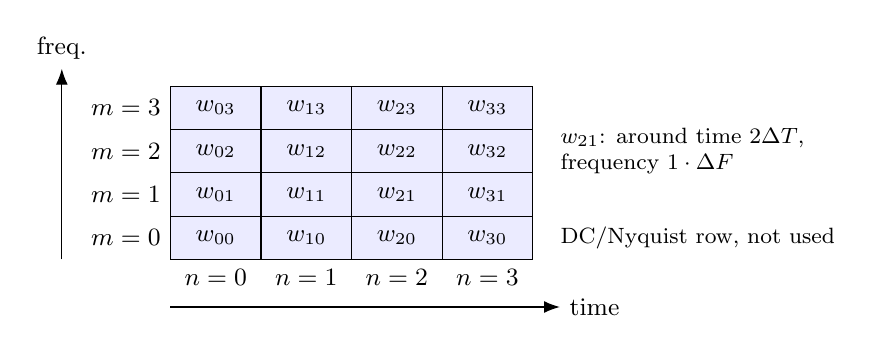
\begin{tikzpicture}[x=1.15cm,y=0.55cm,font=\small]
  \foreach \n in {0,...,3}{\foreach \m in {0,...,3}{
    \draw[fill=blue!8] (\n,\m) rectangle ++(1,1);
    \node at (\n+0.5,\m+0.5) {$w_{\n\m}$};}}
  \foreach \n in {0,...,3}{\node[below] at (\n+0.5,0) {$n=\n$};}
  \foreach \m in {0,...,3}{\node[left] at (0,\m+0.5) {$m=\m$};}
  \node[right,align=left,font=\footnotesize] at (4.2,0.5) {DC/Nyquist row, not used};
  \node[right,align=left,font=\footnotesize] at (4.2,2.5) {$w_{21}$: around time $2\Delta T$,\\ frequency $1\cdot\Delta F$};
  \draw[-{Latex[length=2mm]}] (0,-1.1) -- (4.3,-1.1) node[right] {time};
  \draw[-{Latex[length=2mm]}] (-1.2,0) -- (-1.2,4.4) node[above] {freq.};
\end{tikzpicture}
\end{center}
In the injection runs, $T_{\rm obs}=30$\,d and $\dd t=10$\,s give $N=259{,}200$, and
$N_f=3600$ gives $N_t=72$ pixels of $\Delta T=10$\,h and $\Delta F=13.9\,\mu$Hz. The
same data in the two tilings:
\begin{center}
\begin{tabular}{@{}lcc@{}}
\toprule
 & STFT, two 15-day chunks (Part~I) & WDM, $N_f=3600$ \\
\midrule
time width of a box      & 15\,d & 10\,h \\
frequency height of a box & $0.77\,\mu$Hz & $13.9\,\mu$Hz \\
values                   & $2\times64{,}800$ complex & $72\times3600$ real \\
real numbers in total    & $\approx 2\times64{,}800\times2 = 259{,}200$ & $259{,}200$ \\
\bottomrule
\end{tabular}
\end{center}
Both carry exactly the information of the $259{,}200$ samples. The STFT spends it on
frequency resolution; WDM trades frequency resolution for a time resolution 36 times
better, which is what a modulation that changes over days needs. The count also
explains a factor that will matter in \cref{sec:wmatch}: a complex STFT value is
\emph{two} real numbers, a WDM pixel is \emph{one}.

\subsection{Computing the coefficients}\label{sec:wdmalgo}

\paragraph{Definition.} Each coefficient is one inner product with the \emph{whole}
series:
\begin{equation}
  w_{j,nm} = \sum_{l=0}^{N-1} x_j(t_l)\,g_{nm}(t_l).
  \label{eq:wnm}
\end{equation}
It is one \emph{real} number that measures how much the data look like the wave
packet $g_{nm}$, i.e.\ how much they oscillate at frequency $f_m$ around time $t_n$.
Nothing is cut into segments: the time localisation comes from the shape of $g_{nm}$,
which is negligible far from $t_n$. Evaluated literally, \cref{eq:wnm} costs about
$N^2$ operations.

\paragraph{The fast algorithm (\CornishEq{13}).} \texttt{bahamas} computes the same
numbers in the frequency domain, where the window is defined. The STFT works
\emph{time first} (cut a segment, then Fourier transform it); this algorithm works
\emph{frequency first}:
\begin{enumerate}
  \item Fourier transform the \emph{whole} series \emph{once}: $X(f)$, on bins spaced
        $1/(N\dd t)$.
  \item For row $m$, keep the Fourier bins around $f_m$ and multiply them by the
        window $\tilde\phi(f-f_m)$. This is a band-pass filter of width about
        $\Delta F$. One row of pixels is $\Delta F/(1/N\dd t) = N_t/2$ Fourier bins
        tall.
  \item Shift the band to zero frequency and inverse Fourier transform it, with length
        $N_t$. This gives the band's slowly varying signal at the $N_t$ pixel times
        $t_0,\dots,t_{N_t-1}$.
  \item From each of these $N_t$ complex values keep \emph{one} real number: the real
        part if $n+m$ is even (the cosine packet), the imaginary part if $n+m$ is odd
        (the sine packet). This is the alternation of \cref{eq:gnm}, and it keeps the
        total count at $N$.
  \item Repeat for every row $m$.
\end{enumerate}
\textbf{One inverse FFT gives a whole row, not one pixel.} The time index $n$ is the
output index of the inverse FFT. Time is not lost in the spectrum: it is stored in the
\emph{phases} of the Fourier coefficients (a feature at $t_0$ contributes a phase
$e^{-2\pi\imath f t_0}$ that rotates from bin to bin). Inverse-transforming all $N$
bins recovers $N$ samples at spacing $\dd t$; inverse-transforming the $N_t$ bins of
one band recovers that band at the coarser spacing $T_{\rm obs}/N_t=\Delta T$, which is
enough because a narrow band changes slowly. Formally, by Parseval's theorem
\cref{eq:wnm} equals
\[
  w_{nm} \;\propto\; \sum_{f\ \text{near}\ f_m} X(f)\,\tilde\phi(f-f_m)\,
  e^{+2\pi\imath (f-f_m)\,t_n},
\]
and the factor $e^{2\pi\imath(f-f_m)t_n}$, which moves the packet to time $t_n$, is
exactly the kernel of an inverse FFT with output index $n$. So the window picks the
band ($m$) and the inverse FFT slides the packet along time ($n$). The transform is
therefore a \emph{filter bank}: $N_f$ narrow bands, each sampled at $N_t$ times. In the
injection runs, a row is $36$ Fourier bins tall, the code takes $71$ bins around
$f_m$, and each inverse FFT has length $72$.

\subsection{Properties of the WDM transform}

\begin{itemize}
  \item \textbf{Orthonormal and critically sampled:} $N$ real samples in, $N$ real
        coefficients out, $\sum w^2=\sum x^2$, exactly invertible.
  \item \textbf{Real coefficients}, one real Gaussian degree of freedom per pixel for
        Gaussian data.
  \item \textbf{Uniform, adjustable tiling:} all pixels have the same $\Delta T$ and
        $\Delta F$, and $N_f$ trades one against the other.
  \item \textbf{Localised:} each basis function is compact in frequency
        ($|f-f_m|<\tfrac34\Delta F$) and decays quickly in time (a few $\Delta T$), so
        there is little leakage.
  \item \textbf{Nearly diagonal for locally stationary noise:} pixels are almost
        uncorrelated and their variance follows $S(f,t)$ (\Cornish; \cref{sec:wstats}).
  \item \textbf{Fast:} one FFT of length $N$ and $N_f$ inverse FFTs of length $N_t$.
  \item \textbf{Periodic edges:} the FFT treats the series as periodic, so the first
        and last time columns mix the end of the series with its start and are
        discarded (\cref{sec:wstats}).
\end{itemize}
Our implementation follows \Cornish\ and agrees with the \texttt{pywavelet} package
coefficient by coefficient, up to a global factor $\sqrt2$ in their normalisation
(theirs is not orthonormal).

%============================================================================
\section{Statistics of a WDM pixel}\label{sec:wstats}
%============================================================================

The likelihood rests on one statement:
\begin{equation}
  \boxed{\;w_{j,nm}\sim\mathcal N\big(0,\sigma^2_{j,nm}\big),\qquad
  \sigma^2_{j,nm} = \frac{P_j(t_n)\,\langle S^{\rm GF}\rangle_m + \langle S^{(n)}_j\rangle_m}{2\,\dd t},
\;}
  \label{eq:pixvar}
\end{equation}
with different pixels independent. We justify this in four steps.

\paragraph{1. Gaussian, with zero mean.} \Cref{eq:wnm} is a weighted sum of data
samples. The samples are Gaussian (both processes in \cref{eq:xt} are Gaussian, and
multiplying by the fixed curve $\sqrt{P_j(t)}$ keeps them Gaussian), and a weighted
sum of Gaussians is Gaussian. Every term has zero mean. This is the same reason the
Fourier amplitudes of Part~I are Gaussian: the FFT is also a weighted sum.

\paragraph{2. Variance $S/(2\dd t)$.} For white noise of variance $\sigma_x^2$ per
sample, the one-sided PSD $S$ is flat up to the Nyquist frequency $1/(2\dd t)$ and
integrates to the variance, $\sigma_x^2 = S/(2\dd t)$. An orthonormal transform is a
rotation in $N$ dimensions and maps independent $\mathcal N(0,\sigma_x^2)$ samples to
independent $\mathcal N(0,\sigma_x^2)$ coefficients. So $\mathrm{Var}(w)=S/(2\dd t)$.
The same follows from counting energy: a band of width $\Delta F$ carries power
$S\,\Delta F$; over $\Delta T/\dd t$ samples that is an energy $S\Delta F\Delta T/\dd t
= S/(2\dd t)$, and the orthonormal transform puts it into the one coefficient of the
box. For coloured noise a pixel sees the PSD through its window, so $S(f_m)$ is
replaced by the window average
\begin{equation}
  \langle S\rangle_m = \frac{\int S(f)\,|\tilde\phi(f-f_m)|^2\,\dd f}{\int|\tilde\phi(f)|^2\,\dd f},
\end{equation}
evaluated in the code on 17 points across $|f-f_m|<\tfrac34\Delta F$. This matters at
low frequency, where the spectrum is steep and a pixel ($13.9\,\mu$Hz) is 14\% of the
frequency at $0.1$\,mHz. The cosine and sine packets carry the same energy, so the
parity of $n+m$ does not affect the variance.

\paragraph{3. The modulation enters as $P_j(t_n)$.} The two components of
\cref{eq:xt} are independent, so their variances add. The Galactic part of $w_{nm}$
is $\sum_l g_{nm}(t_l)\sqrt{P_j(t_l)}\,g_j(t_l)$. The packet is non-zero only within a
few $\Delta T$ of $t_n$ (about a day), over which $P_j$ hardly changes, so
$\sqrt{P_j(t_n)}$ can be taken out of the sum. This is the \emph{locally stationary}
approximation; its error grows with the curvature of $P_j$ over a day.

\paragraph{4. Independence (the diagonal approximation).} For white stationary noise
the pixels are exactly independent (orthonormality). For coloured or modulated noise
the cancellations of \cref{sec:wdm} are exact only if the spectrum is flat across the
overlap of two packets, so small correlations could remain. We measured them on 100
fresh simulations of the run-1 setup (30\,d, $N_f=3600$; the injected atoms make the
expected value exact). Correlated pixels would show up as a variance of the grouped
statistic above the Gamma value $2/\nu_g$ (see \cref{sec:wgamma}):
\begin{center}
\small
\begin{tabular}{@{}lcccc@{}}
\toprule
band & median $\nu_g$ & mean $Y/\langle Y\rangle$ & $\nu_g\,\mathrm{Var}(Y/\langle Y\rangle)$ & corr.\ freq / time \\
 & & (expect 1) & (expect 2) & (expect 0) \\
\midrule
0.1--0.3\,mHz & 2  & 1.005 & $2.010\pm0.024$ & $+0.003$ / $+0.001$ \\
0.3--1\,mHz   & 2  & 1.002 & $1.997\pm0.010$ & $-0.002$ / $-0.003$ \\
1--3\,mHz     & 6  & 1.002 & $2.007\pm0.009$ & $+0.000$ / $-0.000$ \\
3--10\,mHz    & 22 & 1.000 & $1.999\pm0.006$ & $+0.000$ / $-0.000$ \\
10--29\,mHz   & 69 & 1.001 & $2.006\pm0.007$ & $+0.000$ / $+0.000$ \\
\bottomrule
\end{tabular}
\end{center}
The effective number of degrees of freedom equals $\nu_g$ to 1\% in every band, even
at the lowest frequencies. The same data give $w^2/\sigma^2$ with mean 1 and variance
2, as $\chi^2_1$ requires. The check covers data simulated from the model itself (no
gaps or glitches) and this grid only.

\paragraph{Edges.} Because the transform is periodic, the first and last time columns
are biased (by $+10\%$ over the band, and up to $+270\%$ below 1\,mHz, in the first
column). From the third column on, every pixel is unbiased, so the likelihood drops
two columns (20\,h) at each end (\texttt{edge\_bins}). An end of the series behaves
like a gap; \cref{sec:gaps} returns to this.

%============================================================================
\section{Coarse graining: grouping pixels}\label{sec:wgroup}
%============================================================================

The 30-day analysis has $2\times68\times2081\approx283{,}000$ pixels in
$[0.1,29]$\,mHz. As in \cref{sec:coarse}, they are coarse grained to make each
likelihood evaluation cheaper. A \textbf{group} is a rectangle of pixels:
\[
  \text{group }(j,s,g) = \underbrace{\texttt{time\_bin}\ \text{consecutive time
  columns}}_{\text{time block } s}\ \times\
  \underbrace{\text{the rows whose } f_m \text{ falls in log bin } g}_{\text{frequency group } g},
\]
and the data enter only through the sum of squares over it,
\begin{equation}
  Y_{j,sg} = \sum_{n\in s}\ \sum_{m\in g} w_{j,nm}^2,
  \qquad \nu_g = \text{number of pixels in the group}.
  \label{eq:Y}
\end{equation}
In the injection runs \texttt{time\_bin}$\,=2$ (blocks of 20\,h) and the band is split
into 200 log-spaced bins of equal width in $\log f$ (2.9\% each). At low frequency a log
bin is narrower than one pixel, so it contains one row or none; empty bins are
dropped, leaving 174 groups. $\nu_g$ grows from 2 (one row $\times$ two columns) at
the bottom to 116 at the top. The likelihood then has
$2\times34\times174\approx11{,}800$ terms. Neither 200 nor 2 was tuned; they are a
speed--accuracy compromise (see the end of this section).

\paragraph{Two different averages of the model.} On the data side, \cref{eq:Y} is a
plain sum. On the model side, two averages appear and should not be confused:
\begin{enumerate}
  \item \emph{Inside one pixel}, the window average $\langle S\rangle_m$ of
        \cref{sec:wstats}. It describes what a single pixel measures and is needed even
        without grouping.
  \item \emph{Across the pixels of a group}, the plain mean
        $\bar S_g = \nu_g^{-1}\sum_{m\in g}\langle S\rangle_m$ (counted once per row).
        It exists only because of grouping.
\end{enumerate}
The modulation is \emph{not} averaged over a block: it is evaluated once, at the
block's mean time $\bar t_s$. The model variance of a group is
\begin{equation}
  \sigma^2_{j,sg} = \frac{P_j(\bar t_s)\,\bar S^{\rm GF}_g + \bar S^{(n)}_{j,g}}{2\,\dd t}.
  \label{eq:siggroup}
\end{equation}

\begin{center}
\renewcommand{\arraystretch}{1.25}
\small
\begin{tabular}{@{}p{0.2\textwidth}p{0.36\textwidth}p{0.36\textwidth}@{}}
\toprule
 & chunked (Part~I) & wavelet \\
\midrule
data in one term & $\Pbar = $ mean of $|\tilde d_k|^2$ over a log bin & $Y=$ sum of $w^2$ over a rectangle \\
model within one value & $S$ at the bin midpoint & window average $\langle S\rangle_m$ per pixel \\
model across the term & one midpoint value & mean of $\langle S\rangle_m$ over the group \\
time dependence & $\Mbar^c_j$, averaged over a 15-day chunk & $P_j(\bar t_s)$, at the centre of a 20-h block \\
\bottomrule
\end{tabular}
\end{center}

\paragraph{Are the variances inside a group equal?} The model assumes so (one
$\sigma^2$ per group); in reality the PSD changes slightly from row to row and $P_j$
across a block. For the run settings the largest spread of $\sigma^2$ inside a group
is 0.3\% below 0.3\,mHz, 3--4\% up to 3\,mHz, 10\% above 10\,mHz and 15\% around the
knee of the Galactic spectrum (3--10\,mHz); $P_j$ changes by at most 1.7\% over a
block. Three consequences:
\begin{itemize}
  \item the mean is exact: $\langle Y\rangle=\sum\sigma^2_{nm}=\nu_g\bar\sigma^2$
        whatever the spread;
  \item the variance of $Y$ exceeds the Gamma value by the factor $1+\mathrm{CV}^2$,
        with CV the relative spread of the $\sigma^2$: at most 1.002 here;
  \item information can be lost. If the $\nu_g$ variances are truly equal, $Y$ is a
        \emph{sufficient statistic}: summing loses nothing. If they differ, how
        $\sigma^2$ varies \emph{inside} the group is discarded. The 15\% spread around
        the knee may cost some precision on $f_{\rm knee}$; a run without grouping
        would settle it.
\end{itemize}

%============================================================================
\section{Why the grouped statistic is Gamma distributed}\label{sec:wgamma}
%============================================================================

We now show, step by step, that if $w_1,\dots,w_\nu$ are independent and each
$w_i\sim\mathcal N(0,\sigma^2)$ with the \emph{same} $\sigma^2$, then
\begin{equation}
  Y = \sum_{i=1}^{\nu} w_i^2 \ \sim\ \mathrm{Gamma}\!\left(k=\frac{\nu}{2},\ \vartheta = 2\sigma^2\right).
  \label{eq:Ygamma}
\end{equation}

\paragraph{Step 1: the tool.} The moment generating function (MGF) of a random
variable $X$ is $M_X(t)=\langle e^{tX}\rangle$, a function of the real number $t$. Two
facts are all we need:
\begin{itemize}
  \item[(A)] \emph{It is a fingerprint:} two distributions with the same MGF (on an
        interval around $t=0$) are the same distribution.
  \item[(B)] \emph{Sums become products:} if $X_1$ and $X_2$ are independent,
        \[
          M_{X_1+X_2}(t)=\langle e^{tX_1}e^{tX_2}\rangle=\langle e^{tX_1}\rangle\langle e^{tX_2}\rangle
          = M_{X_1}(t)\,M_{X_2}(t).
        \]
        The middle equality, ``the mean of a product of independent quantities is the
        product of their means'', is the only place where independence is used.
\end{itemize}

\paragraph{Step 2: one squared pixel.} With the Gaussian density of $w$,
\[
  \langle e^{tw^2}\rangle = \int_{-\infty}^{\infty}\frac{1}{\sqrt{2\pi\sigma^2}}\,
  e^{-w^2/(2\sigma^2)}\,e^{tw^2}\,\dd w
  = \int_{-\infty}^{\infty}\frac{1}{\sqrt{2\pi\sigma^2}}\,
  e^{-w^2\left(\frac{1}{2\sigma^2}-t\right)}\,\dd w .
\]
For $t<1/(2\sigma^2)$ the integrand is again a Gaussian shape, with a new variance
$\sigma'^2$ defined by $\frac{1}{2\sigma'^2}=\frac{1}{2\sigma^2}-t$, i.e.\
$\sigma'^2=\sigma^2/(1-2\sigma^2t)$. Using $\int e^{-w^2/(2\sigma'^2)}\dd w=\sqrt{2\pi\sigma'^2}$,
\[
  \langle e^{tw^2}\rangle = \sqrt{\frac{\sigma'^2}{\sigma^2}} = (1-2\sigma^2t)^{-1/2}.
\]

\paragraph{Step 3: the sum.} By (B), the MGF of $Y$ is the product of $\nu$ identical
factors:
\[
  M_Y(t) = \big[(1-2\sigma^2t)^{-1/2}\big]^{\nu} = (1-2\sigma^2t)^{-\nu/2}.
\]
This step also needs all $\nu$ variances to be \emph{equal}; otherwise the factors
differ and do not combine into one power.

\paragraph{Step 4: the MGF of a Gamma distribution.} With the density of
Part~I, $p(x\mid k,\vartheta)=x^{k-1}e^{-x/\vartheta}/(\Gamma(k)\vartheta^k)$ for $x>0$,
and the standard integral $\int_0^\infty x^{k-1}e^{-ax}\dd x=\Gamma(k)/a^k$,
\[
  M(t) = \frac{1}{\Gamma(k)\vartheta^k}\int_0^\infty x^{k-1}e^{-x\left(\frac1\vartheta-t\right)}\dd x
  = \frac{1}{\Gamma(k)\vartheta^k}\,\frac{\Gamma(k)}{(1/\vartheta-t)^{k}}
  = (1-\vartheta t)^{-k}.
\]

\paragraph{Step 5: match.} Steps 3 and 4 are the same function when $k=\nu/2$ and
$\vartheta=2\sigma^2$. By (A), \cref{eq:Ygamma} holds. Equivalently,
$Y/\sigma^2\sim\chi^2_\nu$, the chi-squared distribution with $\nu$ degrees of freedom.

\paragraph{Step 6: sanity check.} The Gamma mean is
$k\vartheta=\tfrac{\nu}{2}\cdot2\sigma^2=\nu\sigma^2$, as it should be for $\nu$ terms of
mean $\sigma^2$. The variance is $k\vartheta^2=2\nu\sigma^4$, so
\[
  \mathrm{Var}\!\left(\frac{Y}{\langle Y\rangle}\right)=\frac{2\nu\sigma^4}{\nu^2\sigma^4}=\frac2\nu,
  \qquad\text{i.e.}\qquad \nu\,\mathrm{Var}\!\left(\frac{Y}{\langle Y\rangle}\right)=2,
\]
which is the quantity measured in \cref{sec:wstats}.

\begin{keybox}[Assumptions used]
(i) each $w$ is Gaussian with zero mean (Step~2; \cref{sec:wstats}, point~1);
(ii) the $\nu$ pixels are independent (Step~3, fact~B; checked in \cref{sec:wstats});
(iii) they share one variance (Step~3; true to 0.2\% in variance, \cref{sec:wgroup}).
\end{keybox}

%============================================================================
\section[The wavelet likelihood and its equivalence with Eq.~(9)]{The wavelet likelihood and its equivalence with \PoneEq{9}}\label{sec:wmatch}
%============================================================================

\subsection{The likelihood}

Taking the logarithm of the Gamma density with $k=\nu_g/2$ and $\vartheta=2\sigma^2$,
and summing over channels, blocks and groups (independent by \cref{sec:wstats}):
\begin{equation}
  \log\mathcal L(\boldsymbol Y\mid\theta) = \sum_{j,s,g}\left[
  \left(\frac{\nu_g}{2}-1\right)\log Y_{j,sg} - \frac{Y_{j,sg}}{2\sigma^2_{j,sg}}
  - \log\Gamma\!\left(\frac{\nu_g}{2}\right) - \frac{\nu_g}{2}\log\big(2\sigma^2_{j,sg}\big)\right],
  \label{eq:wlik}
\end{equation}
with $\sigma^2_{j,sg}(\theta)$ from \cref{eq:siggroup}. This is exactly what the code
evaluates (\texttt{model.py} in \texttt{bahamas/wavelet}; the terms without $\theta$ are computed
once, the two with $\sigma^2$ at every call). As in Part~I, $Y$ is the \textbf{data}
and $\sigma^2(\theta)$ the \textbf{model}.

\subsection[Rewriting it in the variables of Eq.~(9)]{Rewriting it in the variables of \PoneEq{9}}

To compare with \cref{eq:gamma} we relabel its coarse bin $m\to g$ and its chunk
$c\to s$. For one term (indices dropped), \cref{eq:gamma} reads
\begin{equation}
  \ell_{\rm Eq.\,9} = -\left[\log\Gamma\!\left(\frac{n}{2}\right) + \frac n2\log S
  - \left(\frac n2-1\right)\log\Pbar + \frac n2\,\frac{\Pbar}{S}\right],
  \label{eq:eq9one}
\end{equation}
and one term of \cref{eq:wlik} is
\begin{equation}
  \ell_{\rm wdm} = \left(\frac{\nu}{2}-1\right)\log Y - \frac{Y}{2\sigma^2}
  - \log\Gamma\!\left(\frac{\nu}{2}\right) - \frac{\nu}{2}\log(2\sigma^2).
  \label{eq:wone}
\end{equation}
We look for a data variable $\Pbar_w$ (built from $Y$) and a model variable $S_w$
(built from $\sigma^2$) that turn \cref{eq:wone} into \cref{eq:eq9one} with
$n\to\nu$.

\paragraph{Step 1: the $\log S$ term.} \Cref{eq:wone} contains
$-\frac\nu2\log\sigma^2$ (from $-\frac\nu2\log2\sigma^2=-\frac\nu2\log2-\frac\nu2\log\sigma^2$),
and \cref{eq:eq9one} contains $-\frac\nu2\log S_w$. They agree up to a constant for
\emph{any} proportionality
\[
  S_w = \kappa\,\sigma^2,\qquad \kappa>0\ \text{a constant},
\]
because $-\frac\nu2\log S_w = -\frac\nu2\log\sigma^2-\frac\nu2\log\kappa$. This term
alone does not fix $\kappa$.

\paragraph{Step 2: the data term.} Matching $-Y/(2\sigma^2)$ with
$-\frac\nu2\Pbar_w/S_w$ and inserting $S_w=\kappa\sigma^2$:
\[
  \frac{Y}{2\sigma^2} = \frac\nu2\,\frac{\Pbar_w}{\kappa\sigma^2}
  \quad\Longrightarrow\quad
  \Pbar_w = \frac{\kappa\,Y}{\nu}.
\]
So the whole family $(\Pbar_w,S_w)=(\kappa Y/\nu,\ \kappa\sigma^2)$ reproduces the two
$\theta$-dependent terms of \cref{eq:eq9one}.

\paragraph{Step 3: the remaining terms.} With $Y=\nu\Pbar_w/\kappa$,
\[
  \left(\frac\nu2-1\right)\log Y = \left(\frac\nu2-1\right)\log\Pbar_w
  + \left(\frac\nu2-1\right)\log\frac{\nu}{\kappa},
\]
and $-\log\Gamma(\nu/2)$ is common to both. Collecting everything,
\begin{equation}
  \ell_{\rm wdm} = \ell_{\rm Eq.\,9}\Big|_{n\to\nu,\ \Pbar\to\Pbar_w,\ S\to S_w} + C_\nu,
  \qquad
  C_\nu = \left(\frac\nu2-1\right)\log\frac\nu\kappa + \frac\nu2\log\frac{\kappa}{2}.
  \label{eq:wmatch}
\end{equation}
$C_\nu$ contains neither $\theta$ nor anything that changes during sampling, so it does
not affect the posterior.

\paragraph{Step 4: fixing $\kappa$ by what the symbols mean.} In \PoneEq{9}, $S$ is
the model PSD (in Hz$^{-1}$) and $\langle\Pbar\rangle=S$. Using
$\langle Y\rangle=\nu\sigma^2$ and \cref{eq:siggroup},
\[
  \langle\Pbar_w\rangle = \frac{\kappa}{\nu}\,\nu\sigma^2 = \kappa\sigma^2 = S_w
  \quad\text{(always)},\qquad
  S_w = \frac{\kappa}{2\,\dd t}\Big(P_j\bar S^{\rm GF}_g + \bar S^{(n)}_{j,g}\Big).
\]
$S_w$ is the physical PSD only for $\kappa=2\,\dd t$. Hence
\begin{equation}
  \boxed{\;\Pbar_w = \frac{2\,\dd t\;Y}{\nu},\qquad
  S_w = 2\,\dd t\;\sigma^2 = P_j(\bar t_s)\,\bar S^{\rm GF}_g + \bar S^{(n)}_{j,g},\qquad
  C_\nu = \frac\nu2\log\frac\nu2 - \log\frac{\nu}{2\,\dd t}.\;}
\end{equation}
$\Pbar_w$ is the \emph{wavelet averaged periodogram}: the mean of the $\nu$ values
$2\dd t\,w^2$, each of which has mean $\langle S\rangle_m$, exactly as each
$|\tilde d_k|^2$ has mean $S$. The constant has two parts: $\frac\nu2\log\frac\nu2$,
which \Pone\ also drops (\cref{sec:gamma}), and $-\log\frac{\nu}{2\dd t}$, the Jacobian
of the change of variables $Y\to\Pbar_w$.

\paragraph{A pitfall.} Another member of the family, $\kappa=\nu\,\dd t$, gives
$\Pbar_w=\dd t\,Y$. It reproduces \cref{eq:eq9one} algebraically, but its model is
$S_w=\nu\dd t\,\sigma^2=\frac\nu2(P_j\bar S^{\rm GF}_g+\bar S^{(n)}_{j,g})$, which is not the
PSD unless $\nu=2$. Since the low-frequency groups have $\nu=2$, matching on one of them
gives $\dd t\,Y$ by coincidence; a group with $\nu=69$ shows the difference.

\paragraph{Result.} Summing over $j,s,g$,
\begin{equation}
  \log\mathcal L_{\rm wdm}(\boldsymbol Y\mid\theta) = \sum_s
  \log\mathcal L^{\rm chunk}_G\big(\boldsymbol{\Pbar}_{w,s}\mid\theta\big)\Big|_{n_{b}\to\nu}
  + \text{const}:
\end{equation}
\textbf{the wavelet likelihood is \PoneEq{9} applied to wavelet periodograms, with time
blocks in the role of chunks.} We checked numerically that the code's value equals the
right-hand side to $10^{-12}$.
\begin{center}
\renewcommand{\arraystretch}{1.2}
\begin{tabular}{@{}ll@{}}
\toprule
\Pone & wavelet \\
\midrule
chunk $c$ (15\,d) & time block $s$ (20\,h) \\
coarse bin with $n_b$ Fourier values & frequency group $g$ with $\nu_g$ pixels \\
$\Pbar=\frac{1}{n_b}\sum|\tilde d_k|^2$ (data) & $\Pbar_w=\frac{2\dd t}{\nu_g}\sum w^2$ (data) \\
$S=\Mbar^c_jS^{\rm GF}+S^{(n)}_j$ (model) & $S_w=P_j(\bar t_s)\bar S^{\rm GF}_g+\bar S^{(n)}_{j,g}$ (model) \\
shape $n_b/2$ & shape $\nu_g/2$ \\
\bottomrule
\end{tabular}
\end{center}

\subsection[The degrees of freedom: an error in Eq.~(9)]{The degrees of freedom: an error in \PoneEq{9}}\label{sec:dofbug}

The forms match, but the shape must be half the number of \emph{real} Gaussian
degrees of freedom averaged, and the two domains count differently.
\begin{itemize}
  \item \textbf{WDM.} Each pixel is one real Gaussian, so $Y/\sigma^2\sim\chi^2_\nu$ and
        the shape $\nu_g/2$ is exact (\cref{sec:wgamma}).
  \item \textbf{Fourier.} Each $\tilde d_k$ is complex; in the simulation of
        \cref{sec:data} its real and imaginary parts are independent, each
        $\mathcal N(0,S/2)$. Repeating Steps 2--5 of \cref{sec:wgamma} with
        $\sigma^2=S/2$ and \emph{two} real terms per frequency:
        \[
          |\tilde d_k|^2 = \tfrac S2\,\chi^2_2,\qquad
          \sum_{k=1}^{n_b}|\tilde d_k|^2 = \tfrac S2\,\chi^2_{2n_b},\qquad
          \Pbar = \frac{S}{2n_b}\chi^2_{2n_b}\ \sim\ \mathrm{Gamma}\!\left(k=n_b,\ \vartheta=\frac{S}{n_b}\right),
        \]
        with $\mathrm{Var}(\Pbar)=S^2/n_b$. The correct shape is $n_b$; \PoneEq{9} uses
        $n_b/2$, which implies $\mathrm{Var}(\Pbar)=2S^2/n_b$.
\end{itemize}
The $\theta$-dependent part of either likelihood is
$-(\text{shape})\big[\log S+\Pbar/S\big]$. Halving the shape halves the curvature of
the log-likelihood, which leaves the maximum where it is but makes the posterior widths
about $\sqrt2$ too large (the remark in \cref{sec:gamma}). Counted on the same patch of
the time--frequency plane, a region with $n_b$ complex Fourier values holds $2n_b$ real
numbers and $\nu=2n_b$ WDM pixels, so
\begin{center}
\begin{tabular}{@{}lll@{}}
wavelet & shape $\nu/2 = n_b$ & exact \\
\PoneEq{9} as printed & shape $n_b/2$ & half the exact value \\
\PoneEq{9} corrected & shape $n_b$ & exact \\
\end{tabular}
\end{center}
The wavelet likelihood and the \emph{corrected} chunked likelihood agree exactly.
Measured on simulated chunked data, $n_b\,\mathrm{Var}(\Pbar/S)=1.04\pm0.04$, which is
the value for shape $n_b$, against 2 for shape $n_b/2$. Correcting the shape in the
chunked runs shrinks their widths by $0.70$--$0.73\approx1/\sqrt2$.

\paragraph{In the code.} All three chunked samplers of \texttt{bahamas} implement the
printed shape $n_b/2$. They are in the folder \texttt{bahamas/method}:
\texttt{setting\_hmc.py} (line 112), \texttt{setting\_nessai.py}
(\texttt{gamma\_lik}) and \texttt{setting\_eryn.py}. Here
$n_b$ is the number of Fourier frequencies averaged in a bin (the \texttt{count}
returned by the log-binning function \texttt{average\_log\_chunks}). The wavelet
likelihood is not affected.

\paragraph{A separate bug in the \texttt{eryn} version.} \texttt{setting\_eryn.py}
(lines 138--143) evaluates
\[
  \left(\frac{n_b}{2}-1\right)\log\big(|\Pbar|^2\big) - \frac{n_b}{2}\log S - \log\Gamma\!\left(\frac{n_b}{2}\right) - \frac{|\Pbar|^2}{2S}
  \quad\text{instead of}\quad
  \left(\frac{n_b}{2}-1\right)\log\Pbar - \dots - \frac{n_b}{2}\frac{\Pbar}{S}.
\]
The data passed to it are already the averaged periodogram $\Pbar$, a power; the code
squares it again and drops the factor $n_b$. Since $\Pbar\sim10^{-40}$ for LISA, the
data term $\Pbar^2/S$ is negligible and the log-likelihood reduces to
$-\frac{n_b}{2}\sum\log S$, which grows without bound as $S\to0$. Any chunked
\texttt{eryn} run with the Gamma likelihood is therefore invalid. The HMC and
\texttt{nessai} versions are correct apart from the shape. Neither issue touches the
wavelet pipeline, which uses \texttt{eryn} only as a sampler with its own likelihood.
Both are to be discussed with the authors before the library is changed.

%============================================================================
\section{Inference: reversible-jump MCMC}\label{sec:rj}
%============================================================================

\subsection{The posterior}

The parameters are the spectral ones,
$\theta_{\rm s}=\{\alpha,\mathrm{amp},f_{\rm knee},f_1,f_2,A_{\rm n},P,b_E\}$, and for
each channel the number of atoms $K_j$ and the atoms
$\zeta_{j,k}=(u_{j,k},\log_{10}\tau_{j,k},a_{j,k})$. The posterior is
\begin{equation}
  p\big(\theta_{\rm s},\{K_j,\zeta_{j,1..K_j}\}\mid\boldsymbol Y\big)\ \propto\
  \mathcal L\big(\boldsymbol Y\mid\theta_{\rm s},\{\zeta\}\big)\ \pi(\theta_{\rm s})
  \prod_{j\in\{A,E\}}\Big[\pi(K_j)\prod_{k=1}^{K_j}\pi(\zeta_{j,k})\Big],
\end{equation}
with uniform priors throughout. Its \emph{dimension changes with} $K_j$, which an
ordinary MCMC cannot handle.

\subsection{What reversible jump does}

Reversible-jump MCMC (\href{https://doi.org/10.1093/biomet/82.4.711}{Green 1995})
adds moves that change the dimension. Here they are \emph{birth} and \emph{death}
moves:
\begin{itemize}
  \item a \textbf{birth} proposes $K\to K+1$ by drawing a new atom from its prior;
  \item a \textbf{death} proposes $K\to K-1$ by removing an atom chosen at random.
\end{itemize}
Each is accepted with a Metropolis--Hastings probability built so that the chain
satisfies detailed balance \emph{across} dimensions. Because the new atom is drawn from
its prior, its prior density cancels its proposal density, and the acceptance
probability reduces to the likelihood ratio times the ratio of move-selection
probabilities (with corrections at $K_{\min}$ and $K_{\max}$). A birth is accepted only
if the extra atom improves the fit enough; a death only if removing an atom costs
little. Between jumps, ordinary moves update the parameters at fixed $K$.

The chain then visits each $K$ in proportion to its posterior probability. With a
uniform prior on $K$, the Bayes factor between two numbers of atoms is simply their
posterior odds, read off by counting samples:
\begin{equation}
  \ln\mathcal B(K,K') = \ln\frac{p(K_j=K\mid\boldsymbol Y)}{p(K_j=K'\mid\boldsymbol Y)},\qquad
  p(K_j=K\mid\boldsymbol Y)\approx\frac{\#\{\text{samples with }K_j=K\}}{\#\{\text{samples}\}}.
\end{equation}
No separate evidence computation is needed for each $K$. The probability of $K=0$
measures the evidence for any modulation at all.

\subsection{Implementation and settings}

The sampler is
\href{https://arxiv.org/abs/2303.02164}{\texttt{eryn}} (Karnesis et al.\ 2023), an
ensemble sampler. An \emph{ensemble} is a set of \emph{walkers}, each a full point in
parameter space, that move together; the number of walkers is a setting, not something
that is inferred. The parameters are organised in \emph{branches}:
\begin{itemize}
  \item \texttt{psd}: $\theta_{\rm s}$, one leaf, updated with stretch moves
        (\href{https://doi.org/10.2140/camcos.2010.5.65}{Goodman \& Weare 2010});
  \item \texttt{mod\_A}, \texttt{mod\_E}: one leaf per atom, $K_j$ leaves, updated
        with a Gaussian random walk (step 2\% of each prior width) and with
        birth/death moves per channel.
\end{itemize}
\textbf{Parallel tempering} runs copies of the ensemble at inverse temperatures
$1=\beta_0>\beta_1>\dots$, each sampling $\mathcal L^\beta\pi$; hot copies change $K$
more easily and swap states with colder ones. Only the cold chain ($\beta=1$) samples
the posterior.

\paragraph{One step of the sampler.} For each walker: take the proposed
$\theta_{\rm s}$ and atoms; compute the band-averaged spectra $\bar S^{\rm GF}_g$,
$\bar S^{(n)}_{j,g}$; compute $P_j(\bar t_s)$ from \cref{eq:atoms}; form
$\sigma^2_{j,sg}$ (\cref{eq:siggroup}); evaluate \cref{eq:wlik} against the frozen
$Y$; accept or reject. Nothing is fitted and no data are redrawn. The likelihood is
written in \texttt{jax}: compiled, vectorised over walkers and differentiable. The
fixed-dimension models (no modulation, or the sky envelope of Part~I evaluated at
$\bar t_s$) can also be sampled with NUTS.

\begin{center}
\renewcommand{\arraystretch}{1.15}
\footnotesize
\begin{tabular}{@{}llll@{}}
\toprule
setting & code default & template (1 yr) & injection runs (30 d) \\
\midrule
grid: $N_f$ ($\Delta T$) & --- & 4096 (11.4\,h) & 3600 (10\,h) \\
\texttt{edge\_bins} / \texttt{time\_bin} / \texttt{freq\_bins} & 4 / 1 / per pixel & 4 / 4 / 200 & 2 / 2 / 200 \\
TDI generation & --- & 2 & 1 \\
walkers per temperature & 32 & 32 & 32 \\
temperatures & 1 & 2 & 4 \\
burn-in / stored steps & --- & 1000 / 5000 & 2000 / 6000 \\
$K_j$ range (uniform) & 0--8 & 0--15 & 0--8 \\
atom width $\tau$ (log-uniform) & 5--180\,d & 5--180\,d & 5--60\,d \\
atom amplitude $a$ (uniform) & $[-3,3]$ & $[-3,3]$ & $[-3,3]$ \\
level $b_E$ (uniform) & $[-2,2]$ & $[-2,2]$ & $[-3,3]$ \\
atom centre $u$ (uniform) & $[0,1]$ & $[0,1]$ & $[0,1]$ \\
start & $\theta_{\rm s}$ near injection, $K_j=0$ & same & same \\
\bottomrule
\end{tabular}
\end{center}
Starting at $K_j=0$ tests whether the sampler finds the modulation by itself. Starting
$\theta_{\rm s}$ in a small ball around the injection is a weaker test than a start
from the prior, and is worth changing in later runs.

%============================================================================
\section{The likelihood in the time--frequency plane, and data gaps}\label{sec:gaps}
%============================================================================

\Cref{fig:lgrid} shows what the likelihood reads, for channel A of the run-1 data at
the injected parameters. The left column has every analysed pixel
($68\times2081$), the right column the groups ($34\times174$). The frequency axis is
logarithmic, so low-frequency pixels look taller although all have the same $\Delta F$.

\begin{figure}[t]
\centering
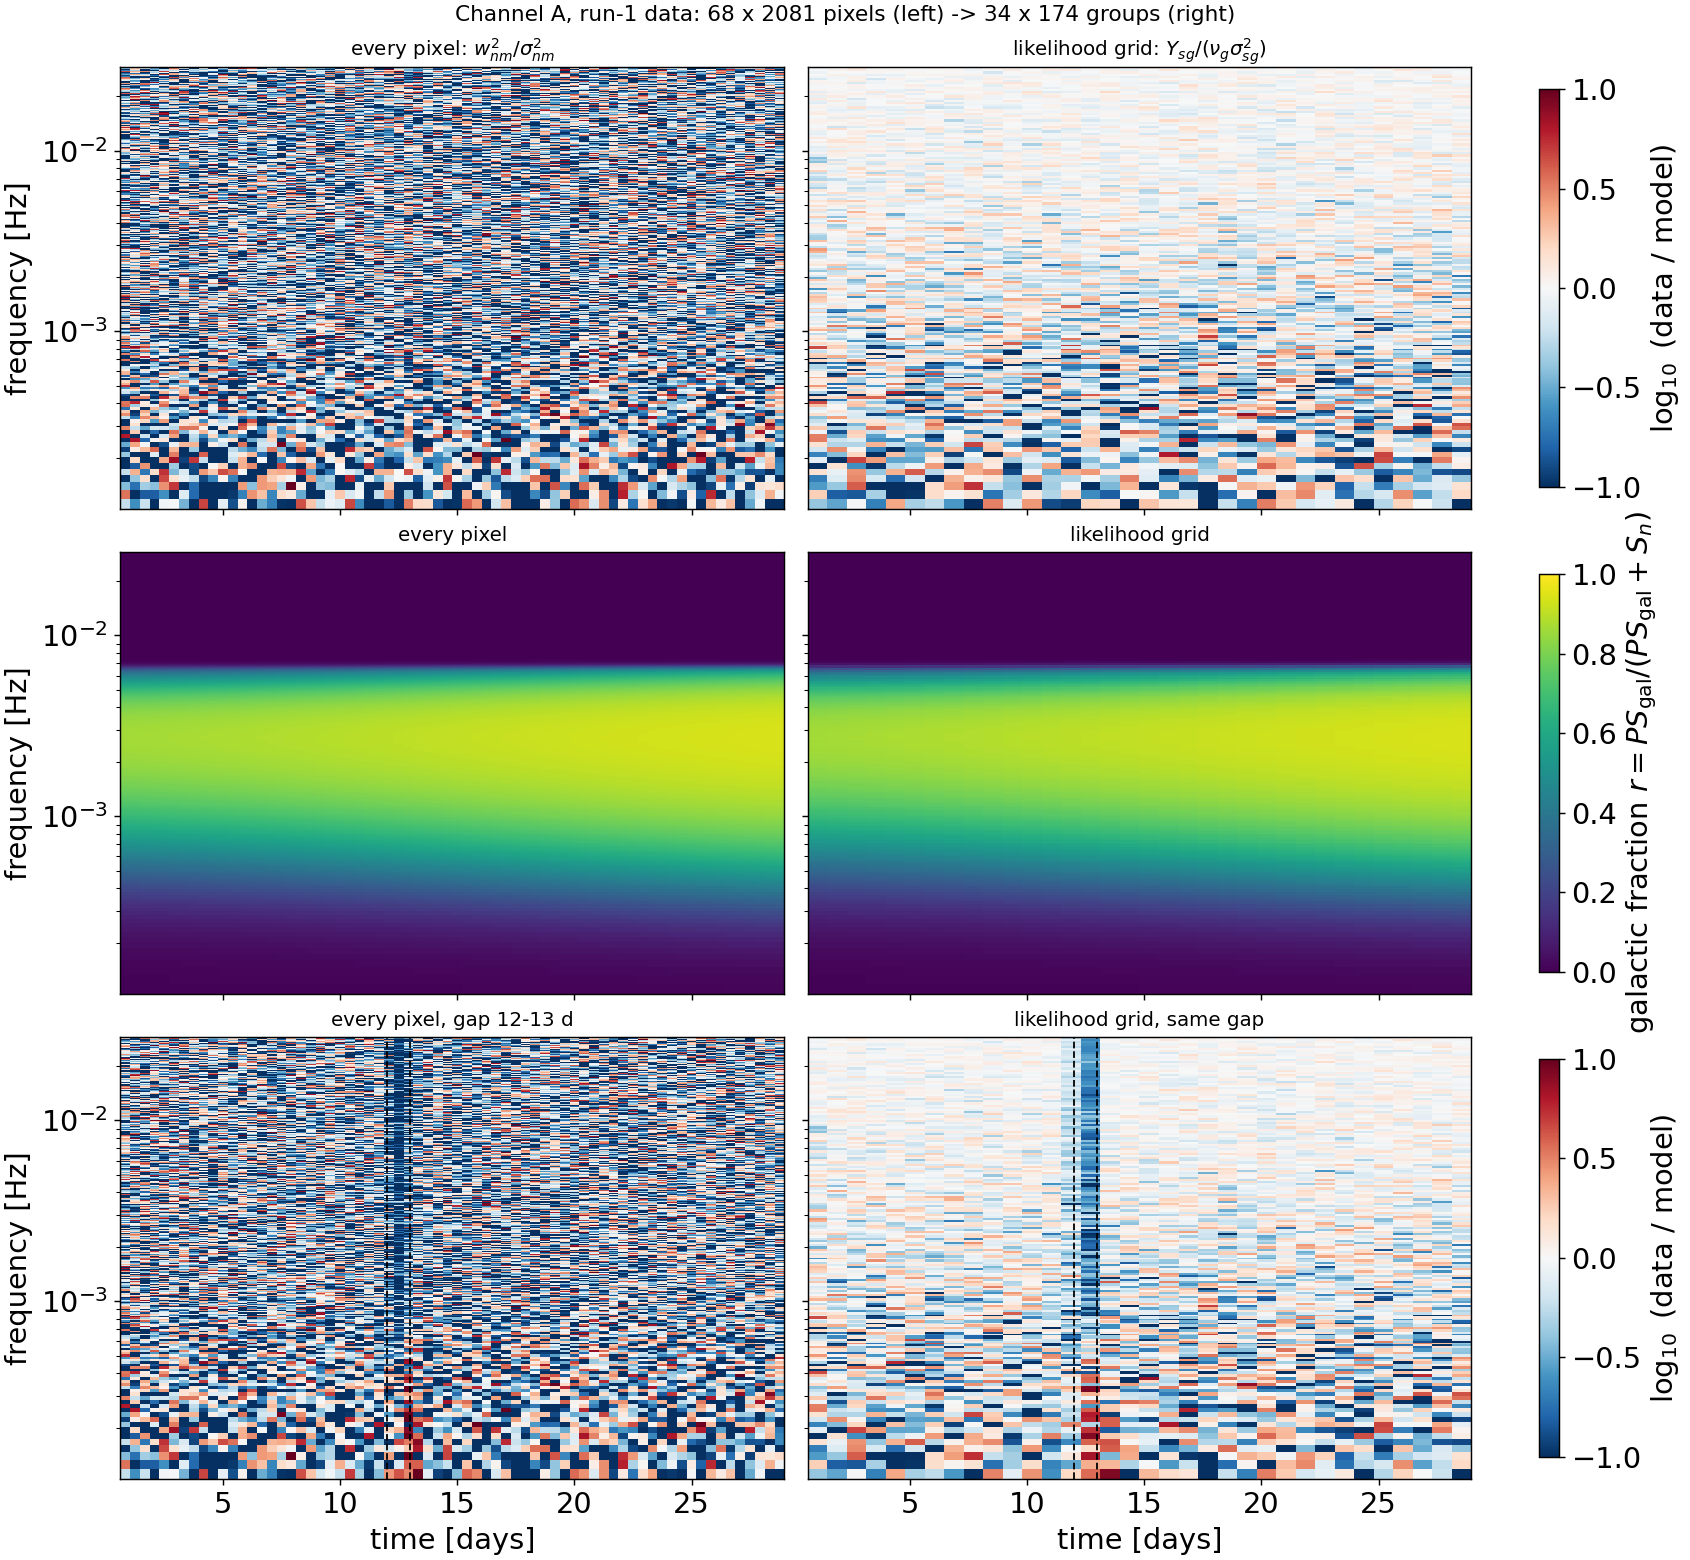
\includegraphics[width=\textwidth]{figures/likelihood_grid.png}
\caption{Channel A, run-1 data, at the injection. Top: data/model, $w^2/\sigma^2$ per
pixel (left) and $Y/(\nu\sigma^2)$ per group (right); white is 1. Middle: Galactic
fraction of the variance, $r=P\,S^{\rm GF}/(P\,S^{\rm GF}+S^{(n)})$. Bottom: as the top
row after setting one day of data (12--13\,d, dashed lines) to zero. Produced by
\texttt{data/wavelet\_injection/likelihood\_grid.py}.}
\label{fig:lgrid}
\end{figure}

\paragraph{Top row: data $\div$ model.} By \cref{sec:wmatch} the likelihood depends on
the data only through this ratio. A single pixel follows $\chi^2_1$ and ranges from
0.01 to 10, so on its own it says almost nothing. Groups scatter by about
$\sqrt{2/\nu_g}$: at the top ($\nu_g\sim70$--$116$) they are within $\sim15\%$ of 1
and look pale; at the bottom ($\nu_g=2$) they stay noisy. At the true parameters there
is no pattern. A wrong model would show one; a stationary model, for example, would
leave a left-to-right colour gradient in the Galactic band.

\paragraph{Middle row: where the Galaxy is learned.} The Fisher information on the
Galactic amplitude carried by a pixel is $r^2/2$. The Galaxy dominates between about
0.4 and 6\,mHz; above the knee ($\approx6.7$\,mHz) the Galactic model drops steeply and
the pixels contain only instrument noise, and below 0.3\,mHz the noise dominates
again. \emph{The modulation is measured almost entirely in the 0.4--6\,mHz band.}
Grouping does not move this information; it summarises it.

\paragraph{Bottom row: a one-day gap.} The gap was made by setting the samples to zero,
with hard edges. Above 1\,mHz the pixels inside the gap drop to 0.1--0.4 of the model
(the power is missing), and the column on each side is slightly low (0.85--0.94): the
damage is \emph{local}, the gap plus about one 10-h pixel on each side, because each
packet spans a few $\Delta T$. Below 1\,mHz the two columns at the end of the gap are
\emph{too high} (about 3 and 2 times the model): zeroing creates a step, a step leaks
power over many frequencies, and the leakage stands out where the spectrum is steep.
This is the same leakage as with the rectangular chunks of Part~I. On the right, a
block that only partly overlaps the gap is biased as a whole.

\paragraph{What this suggests for gaps.}
\begin{enumerate}
  \item \textbf{Mask, do not fill.} Since the pixels are independent, leaving the
        affected terms out of the sum is exact. This is what \texttt{edge\_bins}
        already does at the two ends of the series. In the Fourier domain a gap breaks
        the orthogonality of all frequencies of the chunk; in the WDM domain the damage
        is confined to a strip about a day wide.
  \item \textbf{Leave a margin}: one pixel on each side above 1\,mHz; more below, unless
        the edges are tapered.
  \item \textbf{Taper the gap edges} (as the Tukey taper does for the chunks) to remove
        the low-frequency leakage.
  \item \textbf{Make the grouping gap-aware}: sum only the unmasked pixels of a group and
        set $\nu_g$ to their number. \Cref{eq:Ygamma} holds for any $\nu$.
  \item \textbf{Compared with chunks}: a chunked analysis places its 15-day chunks
        between gaps, so a short gap can cost most of a chunk; here the unit of data
        lost is 10\,h. The atom model of $P_j(t)$ is continuous across a gap; the side of
        a gap behaves like an end of the series, where the atom model is least
        constrained.
\end{enumerate}
Points 1, 2 and 4 are now implemented and are described in Part~III; tapering is
not. Bayesian gap filling in the time--frequency domain
(\href{https://arxiv.org/abs/2509.05479}{Pearson \& Cornish 2025}) is the more complete
alternative to masking.

%============================================================================
\section{Summary of the wavelet pipeline}
%============================================================================

\begin{keybox}[The wavelet pipeline in eight steps]
\begin{enumerate}
  \item Simulate one continuous series per channel, $x_j=n_j+\sqrt{P_j(t)}\,g_j$
        (\cref{eq:xt}), with $P_j$ the true envelope or a set of fitted atoms.
  \item WDM-transform it once: one FFT, then for each row a windowed band, an inverse
        FFT of length $N_t$ and the real or imaginary part by the parity of $n+m$
        (\cref{sec:wdmalgo}).
  \item Drop the edge columns and the rows outside the band.
  \item Group pixels into blocks $\times$ log-frequency groups and keep
        $Y_{j,sg}=\sum w^2$ and $\nu_g$ (\cref{eq:Y}). Steps 1--4 are done once.
  \item For a trial point (spectral parameters, $K_j$ and atoms), compute
        $P_j(\bar t_s)$ from the atoms and the band-averaged spectra.
  \item Form $\sigma^2_{j,sg}$ (\cref{eq:siggroup}).
  \item Evaluate the Gamma likelihood (\cref{eq:wlik}), which is \PoneEq{9} with the
        correct degrees of freedom.
  \item Let \texttt{eryn} propose the next point, including births and deaths of
        atoms, and return to step~5.
\end{enumerate}
\end{keybox}

\paragraph{Status.} All injection runs of Part~V use the envelope code with the
corrections listed in \texttt{reports/PAPER\_BUGS.md}.

\clearpage
%############################################################################
\part{Data gaps in the WDM domain}
%############################################################################

%============================================================================
\section{Injecting a gap and masking it}\label{sec:gapmask}
%============================================================================

LISA will not deliver an uninterrupted stream. Antenna repointings, maintenance and
unplanned events will interrupt the data for hours to days, and the planned duty
cycle is about 75\%. \Cref{sec:gaps} showed that in the WDM domain a gap damages only
the pixels near it. Here we turn that observation into a likelihood and test it on
run~2's data with a short gap (run~3) and a long one (run~4).

\paragraph{The gap in the data.} We take the 30-day series of run~2 (true sky envelope,
same noise realisation) and set it to zero inside the gap:
\begin{equation}
  x_j(t_l) \;\to\; 0 \qquad \text{for } t_{\rm gap,1}\le t_l < t_{\rm gap,2}.
  \label{eq:gapzero}
\end{equation}
Run~3 has a 1-day gap, $[12,13)$\,d (8640 samples per channel); run~4 has a 10-day
gap, $[10,20)$\,d, a third of the window. Outside the gap the series is identical to
run~2's, so any change in the posterior is caused by the gap alone. The zeroed series
is then WDM-transformed as before. The gap has hard edges, the worst case for leakage.

\paragraph{Which pixels are damaged.} Each WDM packet spans a few $\Delta T$, so
pixels whose packets overlap the gap see less than their full share of data. We
measured the bias of each pixel's power, $\langle w^2\rangle/\sigma^2$, over 20 noise
realisations with a 1-day gap:
\begin{itemize}
  \item the 3 time columns that overlap the gap are 60--91\% low (the power is
        missing);
  \item the column just outside on each side is about 10\% low above 1\,mHz, and
        25--40\% \emph{high} below 1\,mHz, where the step at the gap edge leaks the
        steep low-frequency spectrum;
  \item two columns away the bias is below about 2\%, the resolution of 20
        realisations.
\end{itemize}

\paragraph{The mask.} We define a time mask over the WDM columns,
\begin{equation}
  \mu_n = \begin{cases}
    0, & \text{column } n \text{ overlaps the gap, or is its first neighbour on either side},\\
    1, & \text{otherwise},
  \end{cases}
\end{equation}
i.e.\ the gap columns plus one buffer column (10\,h) on each side. The masked columns
are \emph{left out} of the likelihood; they are not set to zero. A zero entering
\cref{eq:wlik} would be read as a \emph{measured} power of zero, and would pull the
modulation down. The mask is the same idea as \texttt{edge\_bins}: an end of the series
is a gap that never closes.

\paragraph{The masked likelihood.} A group of \cref{sec:wgroup} is a time block $s$
(two columns) times the $r_g$ frequency rows of log bin $g$, so $\nu_g=2r_g$. With the
mask, only the kept columns are summed:
\begin{equation}
  Y_{j,sg} = \sum_{n\in s}\mu_n\sum_{m\in g}w^2_{j,nm},\qquad
  \nu_{sg} = r_g\sum_{n\in s}\mu_n,\qquad
  \bar t_s = \frac{\sum_{n\in s}\mu_n t_n}{\sum_{n\in s}\mu_n}.
  \label{eq:Ymask}
\end{equation}
A block with no kept column is dropped. A block with one kept column keeps half its
degrees of freedom, and its modulation is evaluated at the time of that column. The
likelihood is \cref{eq:wlik} with $\nu_g\to\nu_{sg}$ and $P_j(\bar t_s)$ at the
masked block times. This is \emph{exact}, not an approximation: the derivation of
\cref{sec:wgamma} needs only that the summed pixels are independent and share one
variance, and removing pixels from a group keeps both properties. \Cref{eq:Ygamma}
holds for any $\nu$.

\begin{center}
\renewcommand{\arraystretch}{1.15}
\small
\begin{tabular}{@{}lcc@{}}
\toprule
 & run~3 & run~4 \\
\midrule
gap & 12--13\,d (24\,h) & 10--20\,d (240\,h) \\
left out (gap + buffer) & 11.46--13.54\,d (50\,h) & 9.38--20.62\,d (270\,h) \\
time blocks kept & 32 of 34 & 21 of 34 \\
pixels lost & 7.4\% & 39.7\% \\
\bottomrule
\end{tabular}
\end{center}
\Cref{fig:gapmask} shows the two set-ups in the time--frequency plane.

\begin{figure}[t]
\centering
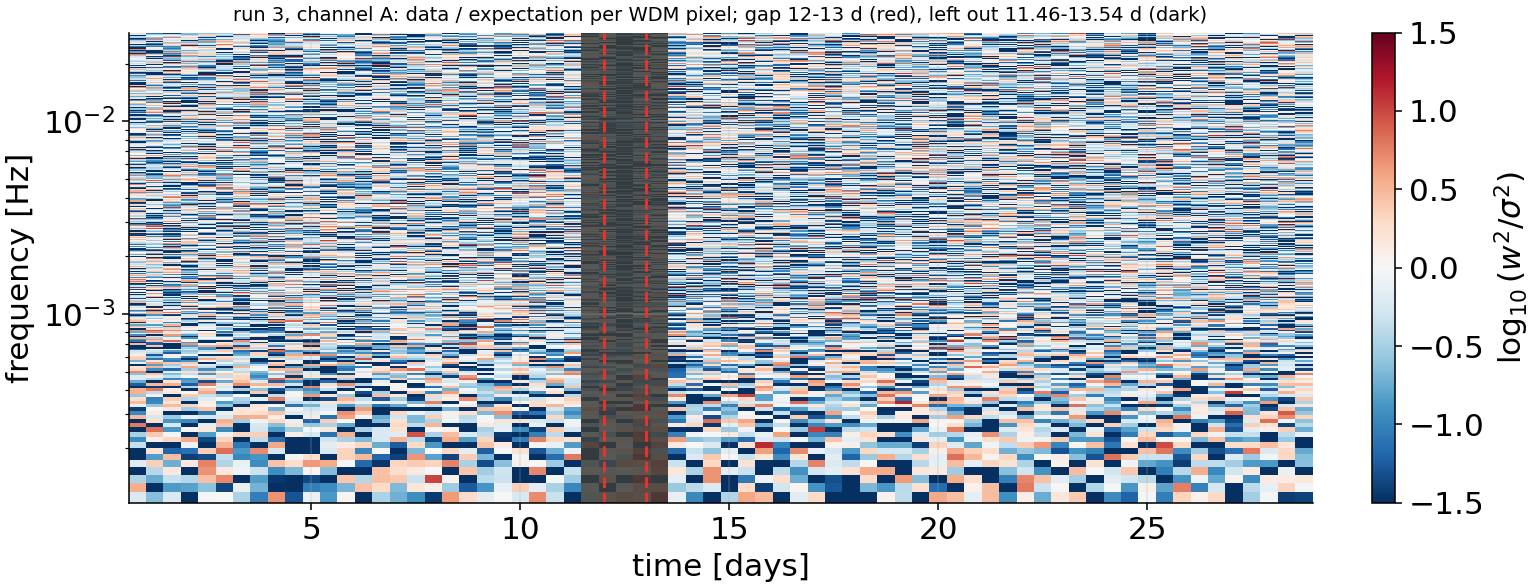
\includegraphics[width=0.92\textwidth]{figures/run3_gap_mask.png}\\[2mm]
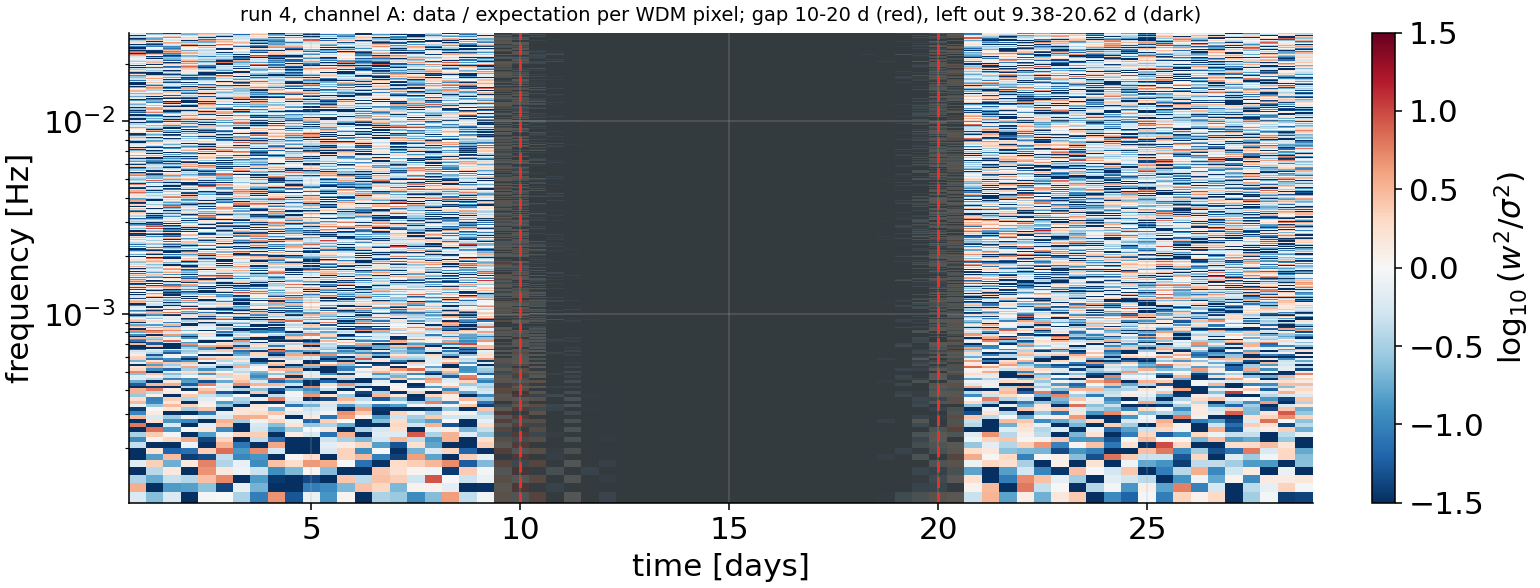
\includegraphics[width=0.92\textwidth]{figures/run4_gap_mask.png}
\caption{Where the gap is injected. Channel A, data/model per WDM pixel,
$\log_{10}(w^2/\sigma^2)$ (white is 1). Red dashed lines: the gap, in which the time
series is set to zero. Dark band: the columns left out of the likelihood (gap plus one
10-h buffer column on each side). Top: run~3, 1-day gap. Bottom: run~4, 10-day gap.}
\label{fig:gapmask}
\end{figure}

%============================================================================
\section{What happens to the modulation inside the gap}\label{sec:gapmod}
%============================================================================

The likelihood has no terms inside the masked region, so the data say nothing about
$P_j(t)$ there. The model, however, is defined at every time. \Cref{eq:atoms} writes
$\ln P_j(t)$ as a sum of Gaussian atoms, a smooth function of $t$ that exists inside
the gap whether or not there are data. Three consequences follow.
\begin{enumerate}
  \item \textbf{Nothing is filled in or interpolated by hand.} The sampler proposes
        atoms exactly as without a gap; the masked likelihood scores them only on the
        kept blocks. The atoms are pinned by the data on both sides of the gap, and
        their values inside the gap follow from their shape.
  \item \textbf{The prior sets how the gap is bridged.} The atom widths are
        log-uniform in 5--60\,d, so every curve the model can draw is smooth on
        day scales. Inside a gap the posterior contains all such curves that join the
        two sides, and its spread is the honest uncertainty of that interpolation. It
        is smallest at the gap edges and largest in the middle. A feature of the
        modulation shorter than the gap could not be recovered inside it; the
        Galactic envelope has none over 30 days.
  \item \textbf{The spectral parameters are shared by all times.} They are measured
        from every kept block, so a gap widens them by roughly
        $\sqrt{1/(1-f_{\rm lost})}$, with $f_{\rm lost}$ the fraction of pixels left
        out, independently of where the gap is.
\end{enumerate}
When we plot the recovered modulation we show it in two ways: with the gap left blank
(only where it is measured), or with the posterior band continued through the gap, as
in \cref{fig:run4mod}, where its width shows how well the atoms bridge it. The chunked
pipeline of Part~I has no such choice: chunks are placed between gaps, and the model
is evaluated only in them.

\clearpage
%############################################################################
\part{Needlets and a patchy Galaxy}
%############################################################################

%============================================================================
\section{From spherical harmonics to needlets}\label{sec:needlets}
%============================================================================

The atom model of \cref{sec:atoms} describes the modulation in \emph{time}, without
reference to the sky. Physically, $P_j(t)$ is the Galaxy's sky distribution seen
through LISA's rotating antenna pattern. The Gaussian Galaxy of \cref{sec:modulation}
is a crude description of that distribution: it has no disk, no bulge, and none of the
satellite galaxies or bar ends that host old stars. To describe the sky without
assuming its shape, in the same spirit as the atoms in time, we need a basis of
functions on the sphere. This section builds one.

\subsection{Spherical harmonics}

The spherical harmonics $Y_{\ell m}(\hat n)$, with multipole $\ell=0,1,2,\dots$ and
$m=-\ell,\dots,\ell$, are the Fourier modes of the sphere. They are the eigenfunctions
of the Laplacian on the sphere, $\nabla^2Y_{\ell m}=-\ell(\ell+1)Y_{\ell m}$, and are
orthonormal and complete:
\begin{equation}
  \int Y_{\ell m}\,Y^*_{\ell'm'}\,\dd\Omega = \delta_{\ell\ell'}\delta_{mm'},\qquad
  f(\hat n) = \sum_{\ell=0}^\infty\sum_{m=-\ell}^{\ell}a_{\ell m}Y_{\ell m}(\hat n),\qquad
  a_{\ell m} = \int f\,Y^*_{\ell m}\,\dd\Omega .
\end{equation}
The multipole $\ell$ plays the role of frequency: a harmonic of degree $\ell$ varies on
angular scales of about $\pi/\ell$. Summing over $m$ gives the \emph{addition
theorem},
\begin{equation}
  \sum_{m=-\ell}^{\ell}Y_{\ell m}(\hat n)\,Y^*_{\ell m}(\hat n')
  = \frac{2\ell+1}{4\pi}\,P_\ell(\hat n\cdot\hat n'),
  \label{eq:addition}
\end{equation}
with $P_\ell$ the Legendre polynomial. So the projection of $f$ onto degree $\ell$ is
$f_\ell(\hat n)=\int\frac{2\ell+1}{4\pi}P_\ell(\hat n\cdot\hat n')f(\hat n')\,\dd\Omega'$,
a kernel that depends only on the angle between the two directions.

Harmonics are perfectly localised in $\ell$, but each one covers the whole sky. A
compact patch of a few degrees therefore needs many harmonics, and a change in one
coefficient changes the map everywhere. The opposite basis, map pixels, is perfectly
local on the sky but says nothing about scale. This is the same dilemma as between a
Fourier transform and a time series in \cref{sec:wdm}, now on the sphere.

\subsection{Needlets}

Needlets (\href{https://doi.org/10.1137/040614359}{Narcowich, Petrushev \& Ward 2006};
\href{https://arxiv.org/abs/0707.0844}{Marinucci et al.\ 2008}) are the sphere's
analogue of the WDM packets: each is concentrated around one direction \emph{and} in
a narrow range of $\ell$. They are built in three steps.

\paragraph{1. Split the multipoles into bands.} Choose a base $B>1$ (we use $B=2$) and
a smooth function $\phi(t)$ that equals 1 for $t\le1/B$, decreases smoothly ($C^\infty$)
to 0 at $t=1$, and is 0 beyond. The window of band $j=0,1,2,\dots$ is
\begin{equation}
  b_j^2(\ell) = \phi\!\left(\frac{\ell}{B^{j+1}}\right) - \phi\!\left(\frac{\ell}{B^{j}}\right),
\end{equation}
which is non-zero only for $B^{j-1}<\ell<B^{j+1}$. A scaling band $j=-1$ with
$b^2_{-1}(\ell)=\phi(\ell)$ collects the largest scales; for $B=2$ it is the monopole
alone. The sum over bands telescopes:
\begin{equation}
  b^2_{-1}(\ell) + \sum_{j=0}^{J}b_j^2(\ell) = \phi\!\left(\frac{\ell}{B^{J+1}}\right) = 1
  \qquad\text{for } \ell\le B^{J}.
  \label{eq:partition}
\end{equation}
The windows form a smooth partition of unity in $\ell$.

\paragraph{2. Build one needlet per band and direction.} For each band, take a set of
$N_j$ directions $\xi_{jk}$ with weights $\lambda_{jk}$ (a cubature rule: the pixel
centres of a HEALPix grid of resolution $n_{{\rm side},j}=2^j$, with
$\lambda_{jk}=4\pi/N_j$; \href{https://arxiv.org/abs/astro-ph/0409513}{G\'orski et al.\ 2005}). The needlet is
\begin{equation}
  \boxed{\;\psi_{jk}(\hat n) = \sqrt{\lambda_{jk}}\sum_{\ell}b_j(\ell)\,
  \frac{2\ell+1}{4\pi}\,P_\ell(\xi_{jk}\cdot\hat n).\;}
  \label{eq:needlet}
\end{equation}
By \cref{eq:addition} it is the band-$j$ part of a delta function at $\xi_{jk}$, a bump
centred on $\xi_{jk}$ and symmetric around it.

\paragraph{3. Analysis and synthesis.} The coefficients and the reconstruction are
\begin{equation}
  \beta_{jk} = \int f\,\psi_{jk}\,\dd\Omega,\qquad
  f(\hat n) = \sum_{j,k}\beta_{jk}\,\psi_{jk}(\hat n).
  \label{eq:needletsynth}
\end{equation}
The second equation follows in two lines. Inserting \cref{eq:needlet} twice,
\[
  \sum_k\beta_{jk}\psi_{jk}(\hat n) = \sum_{\ell,\ell'}b_j(\ell)b_j(\ell')
  \int\dd\Omega'\,f(\hat n')\sum_k\lambda_{jk}\frac{2\ell+1}{4\pi}P_\ell(\xi_{jk}\cdot\hat n')
  \frac{2\ell'+1}{4\pi}P_{\ell'}(\xi_{jk}\cdot\hat n).
\]
If the cubature integrates exactly the polynomials that appear (degree up to
$2B^{j+1}$), the sum over $k$ is the integral $\int\dd\Omega_\xi$, which by
\cref{eq:addition} and orthogonality gives $\delta_{\ell\ell'}\frac{2\ell+1}{4\pi}
P_\ell(\hat n'\cdot\hat n)$. Hence $\sum_k\beta_{jk}\psi_{jk}=\sum_\ell b_j^2(\ell)f_\ell$,
and summing over $j$ with \cref{eq:partition} returns $f$.

\subsection{Properties}

\begin{itemize}
  \item \textbf{Localised in $\ell$:} band $j$ contains only $B^{j-1}<\ell<B^{j+1}$
        (exactly, by construction).
  \item \textbf{Localised on the sky:} because $b_j$ is smooth, $\psi_{jk}$ decays
        quasi-exponentially away from $\xi_{jk}$, over an angle of about $\pi/B^j$
        (\href{https://doi.org/10.1137/040614359}{Narcowich et al.\ 2006}). Large $j$
        means small, sharp needlets.
  \item \textbf{A tight frame, not an orthonormal basis:} \cref{eq:needletsynth}
        reconstructs any band-limited map with the \emph{same} functions for analysis and
        synthesis, but the needlets overlap and are redundant (there are more
        coefficients than degrees of freedom). For a prior or a sampler this is
        harmless; it means a map has more than one set of coefficients.
  \item \textbf{No preferred direction:} every needlet is axisymmetric about its
        centre, and the construction needs no coordinate patch, unlike wavelets on a
        flat projection of the sky.
  \item \textbf{Nearly uncorrelated coefficients} for an isotropic random field at high
        $j$ (\href{https://doi.org/10.1214/08-AOS601}{Baldi et al.\ 2009}).
\end{itemize}
With $B=2$ and our cubature the bands are:
\begin{center}
\small
\begin{tabular}{@{}cccc@{}}
\toprule
band $j$ & multipoles $\ell$ & $n_{{\rm side},j}$ & number of needlets \\
\midrule
$-1$ & 0 & --- & 1 \\
0 & 1 & 1 & 12 \\
1 & 2, 3 & 2 & 48 \\
2 & 3--7 ($\ell=4$ at full weight) & 4 & 192 \\
3 & 5--15 & 8 & 768 \\
\bottomrule
\end{tabular}
\end{center}
This coarse cubature reconstructs a band-limited map to 3.7\% (0.6\% with twice
$n_{{\rm side},j}$), enough for a parametrisation.

\subsection{Why needlets for the Galactic foreground}\label{sec:whyneedlets}

\paragraph{LISA sees only $\ell=0,2,4$.} In the low-frequency limit the power response
of channel $j$ to a source in direction $\hat n$, averaged over polarisation, is
$R_j(t,\hat n)=F_{+,j}^2+F_{\times,j}^2$. Each antenna pattern
$F_{A}=D_{ab}(t)\,e^A_{ab}(\hat n)$ contracts the detector tensor $D_{ab}$ with a
polarisation tensor, and the polarisation sum
$\sum_A e^A_{ab}e^A_{cd}$ is built from the projector $\delta_{ab}-\hat n_a\hat n_b$: a
polynomial of degree 4 in the components of $\hat n$, even under $\hat n\to-\hat n$. A
polynomial of degree 4 contains only harmonics with $\ell\le4$, and an even one only even
$\ell$. Therefore
\begin{equation}
  R_j(t,\hat n) = \sum_{\ell\in\{0,2,4\}}\sum_m r_{j,\ell m}(t)\,Y_{\ell m}(\hat n),
\end{equation}
which we confirmed numerically on the first-principles response (power at other $\ell$
below $10^{-8}$). Since $P_j(t)\propto\int I(\hat n)R_j(t,\hat n)\,\dd\Omega$, the data
see only the projection of the sky onto these $1+5+9=15$ real harmonics. Everything
else in the map, including the sharp edges of any patch, is invisible to an A/E
auto-power analysis.

\paragraph{Only three bands matter.} Expanding the sky in needlets makes $P_j(t)$
linear in the coefficients,
\begin{equation}
  P_j(t) = \sum_{j',k}\beta_{j'k}\,T_{j,j'k}(t),\qquad
  T_{j,j'k}(t) = \frac{\kappa}{\bar R}\int\psi_{j'k}(\hat n)\,R_j(t,\hat n)\,\dd\Omega,
  \label{eq:needletP}
\end{equation}
($\kappa$ and $\bar R$ are fixed normalisations, \cref{sec:patchsim}). $T$ vanishes
for every band without $\ell=0,2,4$ content: $j=0$ ($\ell=1$) and $j\ge3$
($\ell\ge5$). Only bands $j=-1,1,2$ remain, $1+48+192=241$ coefficients. A Fisher
analysis of 30 days gives them 70\%, 29\% and 1.4\% of the information on the sky,
and it constrains only about 5 independent sky patterns.

\paragraph{Why not harmonics or pixels directly?} Fifteen harmonics would describe what
the data see, but each covers the whole sky, so a prior that says ``the excess is
compact'' cannot be written in them. Pixels allow such a prior, but most pixel
combinations are invisible and the visible ones are not separated from the rest.
Needlets do both: their bands separate visible from invisible scales exactly, and
within a band they are local, so a patch is described by a few nearby coefficients and
the prior can be set per band (for instance $\beta_{jk}\sim\mathcal N(0,s_j^2)$ with
$s_j$ the spread of the smooth Galaxy's own coefficients in that band). Over a year,
LISA's orientation sweeps through 360\textdegree, the response mixes the visible modes
differently with time, and this band-by-band bookkeeping is what lets the model grow
with the data.

%============================================================================
\section{Simulating a Galaxy with patches of excess power}\label{sec:patchsim}
%============================================================================

\paragraph{One spectrum, many places.} All Galactic power comes from unresolved
double white dwarfs with the common spectrum $S^{\rm GF}(f)$ of \cref{eq:sgf}. The
components of the sky differ only in \emph{where} the power sits. The sky is a HEALPix
map $I(\hat n)$ of flux per pixel ($n_{\rm side}=64$, 0.9\textdegree\ pixels), and the
modulation is linear in it:
\begin{equation}
  P_j(t) = \frac{\kappa}{\bar R}\sum_{\rm pix}I({\rm pix})\,R_j(t,{\rm pix}),\qquad
  R_j = F_{+,j}^2+F_{\times,j}^2 .
  \label{eq:Pmap}
\end{equation}
$R_j$ is computed from first principles: arm unit vectors from the \texttt{bahamas}
spacecraft orbit, Michelson responses $X,Y,Z$, and then
$A=(Z-X)/\sqrt2$, $E=(X-2Y+Z)/\sqrt6$. $\bar R$ is the all-sky mean of $R_A$, so an
isotropic sky of unit flux gives $P_A=P_E=1$. Because $R_j$ has only $\ell\le4$, the
map can be degraded to $n_{\rm side}=32$ for this sum without any loss.

\paragraph{The smooth Galaxy} is run~2's: the bivariate Gaussian of
\cref{sec:modulation} in ecliptic $(\beta,\lambda)$ with the pack-2 sky parameters,
written out pixel by pixel. Since the envelope formula integrates $p(\beta,\lambda)$ with
the measure $\cos\beta\,\dd\beta\,\dd\lambda$, the flux per pixel is
$p(\beta,\lambda)\,\Delta\Omega$, normalised to a total of 1. The constant $\kappa$ is
fitted once so that this map reproduces run~2's analytic $M_j^2(t)$; it does so to
0.1\% (A) and 0.2\% (E) over the 30 days. The smooth part of the run-5 sky is
therefore exactly run~2's injection, at the same amplitude.

\paragraph{Patches.} Each patch $i$ is an elliptical Gaussian on the sphere centred on
galactic $(l_i,b_i)$. For a pixel at angular distance $\theta$ from the centre and
position angle $\varphi$ (from galactic north towards increasing $l$),
\begin{equation}
  I_i(\hat n) = F_i\,\frac{G_i(\hat n)}{\sum_{\rm pix}G_i},\qquad
  G_i = \exp\!\left[-\frac12\left(\frac{\theta\cos(\varphi-\varphi_i)}{\sigma_{{\rm maj},i}}\right)^2
  -\frac12\left(\frac{\theta\sin(\varphi-\varphi_i)}{\sigma_{{\rm min},i}}\right)^2\right],
  \label{eq:patch}
\end{equation}
with widths $\sigma_{\rm maj}$, $\sigma_{\rm min}$ along and across the major axis,
orientation $\varphi_i$, and $F_i$ the patch's flux in units of the smooth Galaxy's.
The full sky is $I=I_{\rm gal}+\sum_iI_i$, and by \cref{eq:Pmap}
\begin{equation}
  P_j(t) = T_{j,{\rm gal}}(t) + \sum_i F_i\,T_{j,i}(t),
  \label{eq:Ptemplates}
\end{equation}
where $T_{j,i}$ is the modulation produced by patch $i$ per unit flux. The time series
is then simulated exactly as in \cref{eq:xt}, $x_j=n_j+\sqrt{P_j(t)}\,g_j$, with the
same seed as run~2: with the patches switched off, the series equals run~2's to
$3\times10^{-5}$.

We place four patches where old stars, and hence white-dwarf binaries, are known to
concentrate:
\begin{center}
\renewcommand{\arraystretch}{1.15}
\small
\begin{tabular}{@{}lcccp{0.36\textwidth}@{}}
\toprule
patch & $(l,b)$ & $\sigma_{\rm maj}\times\sigma_{\rm min}$ & $F_i$ & why \\
\midrule
LMC & $(280.5^\circ,-32.9^\circ)$ & $3.0^\circ\times2.2^\circ$ & 0.20 & largest satellite galaxy \\
SMC & $(302.8^\circ,-44.3^\circ)$ & $1.6^\circ\times1.0^\circ$ & 0.08 & 20\textdegree\ from the LMC: two patches that blend at low $\ell$ \\
Sgr dSph & $(5.6^\circ,-14.2^\circ)$ & $4.0^\circ\times1.5^\circ$ & 0.12 & on top of the smooth Galaxy, elongated across the plane \\
bar end & $(27^\circ,0^\circ)$ & $6.0^\circ\times1.5^\circ$ & 0.12 & in-plane overdensity that the Gaussian lacks \\
\bottomrule
\end{tabular}
\end{center}
The fluxes are deliberately exaggerated. With the same number of binaries per stellar
mass, the realistic flux fraction is $M/d^2$ relative to the Milky Way: about
$6\times10^{-4}$ for the LMC and below $10^{-4}$ for the SMC and Sgr, hundreds to
thousands of times below what 30 days can detect. Over the 30 days the patches add
85\% (A) and 56\% (E) to the mean Galactic power; the largest single contribution is
the LMC's (+41\% in A, +28\% in E). Each patch sits at a different place in the
antenna pattern, so it adds a different, time-dependent amount to A and to E. That
difference is the only handle the data have on where a patch is.

\begin{figure}[t]
\centering
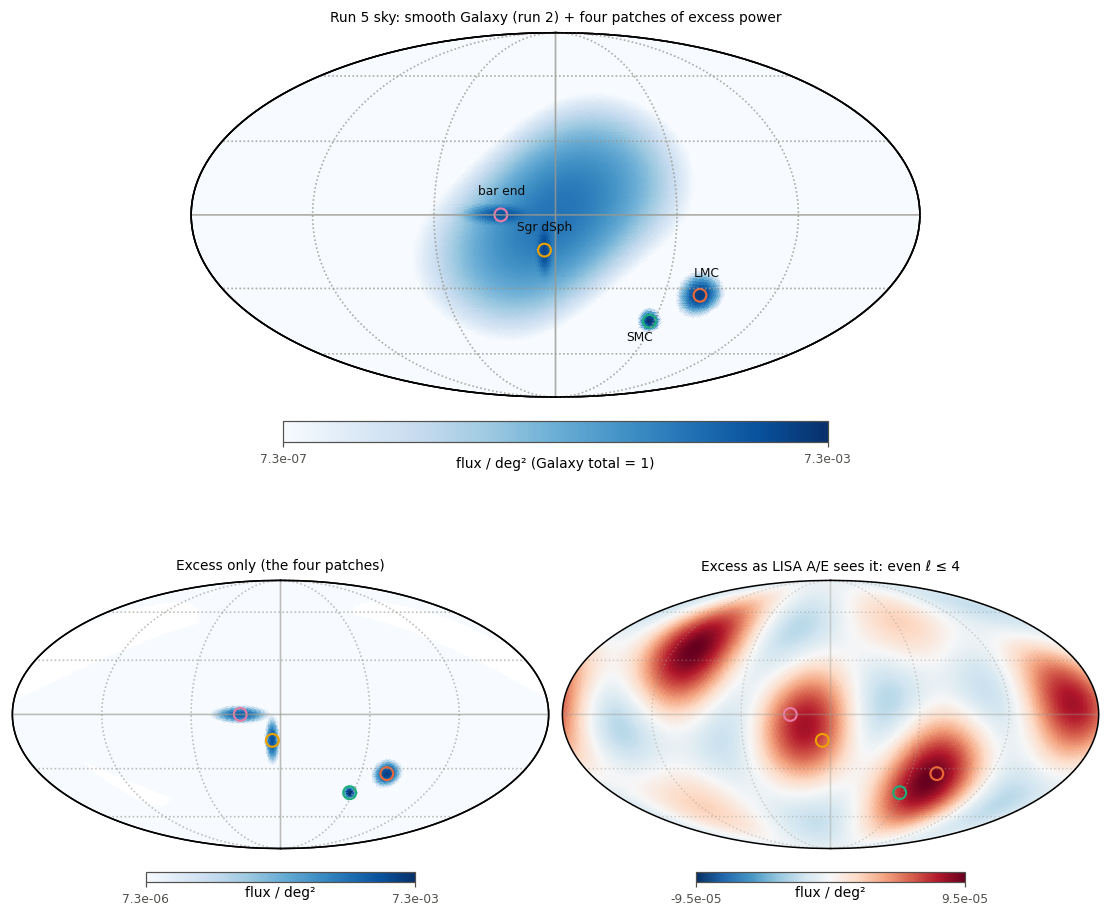
\includegraphics[width=0.85\textwidth]{figures/run5_sky.png}
\caption{The run-5 sky in galactic coordinates. Top: smooth Galaxy (run~2's Gaussian)
plus the four patches, log scale. Bottom left: the patches alone. Bottom right: the
part of the patches LISA's A/E auto-power can see, their projection onto
$\ell=0,2,4$; it holds only 3.5\% of the excess map's power, spread into lobes tens of
degrees wide, and mirrored at the antipodes because the response is even.}
\label{fig:sky}
\end{figure}

%============================================================================
\section{Run 5a: patch fluxes at known positions, and the role of needlets}\label{sec:run5a}
%============================================================================

The plan for run~5 has three steps of increasing freedom: (a) fit the patch fluxes
with positions and shapes known; (b) free the positions; (c) replace the patches by
needlet coefficients in bands $j=-1,1,2$ with a Gaussian prior per band. Only (a) has
been run so far.

\paragraph{The 5a model.} The modulation is \cref{eq:Ptemplates}, with
$T_{j,{\rm gal}}$ fixed at the truth and the patch templates $T_{j,i}$ at their true
positions and shapes. The free parameters are the seven spectral parameters and the
four fluxes $F_i\sim U(0,1)$. The data, the WDM pixels and the Gamma likelihood are
those of runs~1--4; only the model of $P_j(t)$ changes. This is the \emph{best case}
for any sky model: everything about the sky is known except how bright each patch is.
Because the four templates are strongly correlated (below), the posterior is sampled
with NUTS in whitened coordinates: each parameter is mapped from its uniform prior
range to the real line with a logit, and then rotated and scaled with the curvature
of the log-posterior at the truth. Plain NUTS reached its maximum tree depth.

\paragraph{What the needlets explain.} Run~5a does not sample needlets, but the
needlet picture of \cref{sec:whyneedlets} is what explains its result and sets its
place in the plan.
\begin{itemize}
  \item \emph{Only $\ell\le4$ is seen.} A 3\textdegree\ patch enters the data only
        through its $\ell=0,2,4$ projection (\cref{fig:sky}, bottom right), and every
        $T_{j,i}(t)$ is a combination of the same 15 harmonic responses. Over 30 days
        these change little, and each template is a smooth, nearly quadratic curve.
        The templates of different patches, and of the Galaxy, overlap by 79--99\%
        (cosine similarity of the stacked A and E curves). The data can therefore
        measure the total excess well but not how it is split between patches.
  \item \emph{5a is a constrained needlet model.} Each patch map has needlet
        coefficients $\beta^{(i)}_{jk}$, so \cref{eq:Ptemplates} is \cref{eq:needletP}
        with $\beta=\beta^{\rm gal}+\sum_iF_i\beta^{(i)}$: the 241 visible coefficients
        restricted to move along four known directions. Run~5c will free all 241. It
        cannot do better than 5a on the fluxes, so 5a is the benchmark it will be
        compared with.
  \item \emph{Positions are hard.} In the low-frequency limit $R_A+R_E$ depends only on
        the angle between $\hat n$ and the normal to the constellation plane, which
        turns by only about 30\textdegree\ in 30 days. A noise-free scan shows that a
        patch can be moved to any position at the same angle from the normal (a ring
        on the sky) at almost no cost. This is what run~5b will meet, and why a year
        of data, over which the normal precesses through 360\textdegree, is needed to
        localise anything.
\end{itemize}

\clearpage
%############################################################################
\part{Results}
%############################################################################

All runs use 30.00 days of simulated A and E data at $\dd t=10$\,s, TDI generation 1,
seed 2026, simulated with two extra days at each end and cut (non-periodic ends). The
WDM grid has $N_f=3600$ (72 pixels of 10\,h); the likelihood drops two edge columns at
each end and uses 34 blocks of 20\,h $\times$ 174 log-frequency groups in
0.1--29\,mHz. The atom runs use \texttt{eryn} with 32 walkers $\times$ 4 temperatures,
2000 burn-in and 6000 stored steps, starting from $K_j=0$ (\cref{sec:rj}). Every run
is converged: autocorrelation times are at most 8 steps (ESS $\ge24{,}000$) for all
spectral parameters, $K_j$, $\log\mathcal L$ and $P_j(t)$ at several days.

The atom model's \texttt{amp} absorbs the level $b_A$ and trades against the spectral
shape, so it is not compared directly. The modulation is compared through the
\emph{galactic brightness}: for each posterior sample, its amplitude times its
spectral shape (averaged over frequency with the weight of where the Galaxy dominates)
times $P_j(t)$, divided by the injected one. This is the quantity the data constrain.

%============================================================================
\section{Run 1: recovering a modulation made of atoms}
%============================================================================

\paragraph{Set-up.} The injected modulation is the least-squares atom fit to the
true envelope (\cref{sec:atoms}): two atoms in A, one in E, each wider than 23\,d
(\cref{fig:run1inj}). The model can therefore represent the injection exactly.

\begin{figure}[t]
\centering
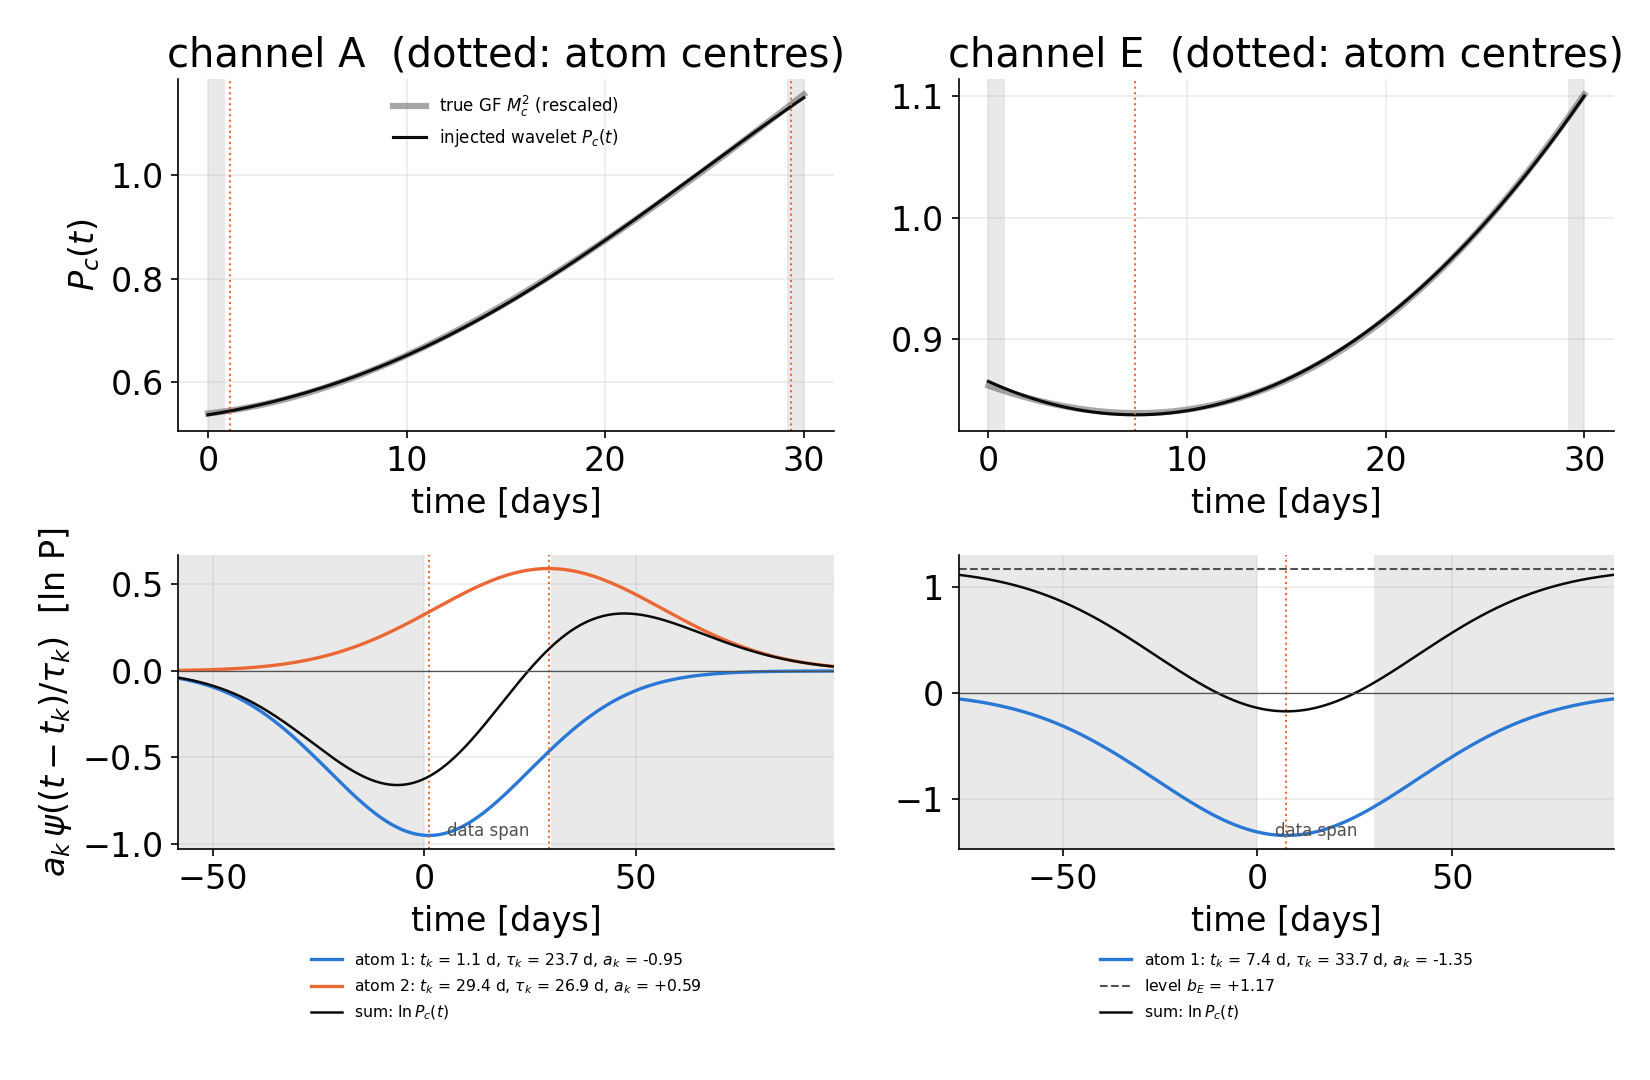
\includegraphics[width=0.9\textwidth]{figures/run1_injection.png}
\caption{Run~1 injection. Top: the injected $P_j(t)$ built from atoms (black) on top
of the true envelope (grey); grey bands are the dropped edge columns. Bottom: the
individual atoms $a_k\psi((t-t_k)/\tau_k)$ in $\ln P$ and their sum, over a range wider
than the data span (white) to show that the atoms extend beyond it.}
\label{fig:run1inj}
\end{figure}

\paragraph{Results.} All eight spectral parameters are recovered within their 90\%
intervals, with every $|z|\le1.3$ (\cref{fig:run1corner}). Starting from $K_j=0$, every
walker finds the modulation within about 50 steps, and $K_j=0$ is never visited
afterwards: the modulation is detected decisively. The number of atoms, however, is
not identifiable: $p(K_A=1)=0.43$ against $p(K_A=2)=0.45$, and similarly in E. Over
30 days the envelope is smooth, and one or two wide atoms draw the same curve. The
single E atom is recovered (centre 7.4\,d inside $[3.6,10.6]$\,d at 90\%); the two A
atoms individually are not. What matters, the galactic brightness, is recovered to
within $\pm1.5\%$ in both channels, with a 90\% band 5.5--5.7\% wide. The one
excursion is A at day~0 (+8\%), where the data would like an atom centre before the
start of the window, which the prior forbids.

\begin{figure}[t]
\centering
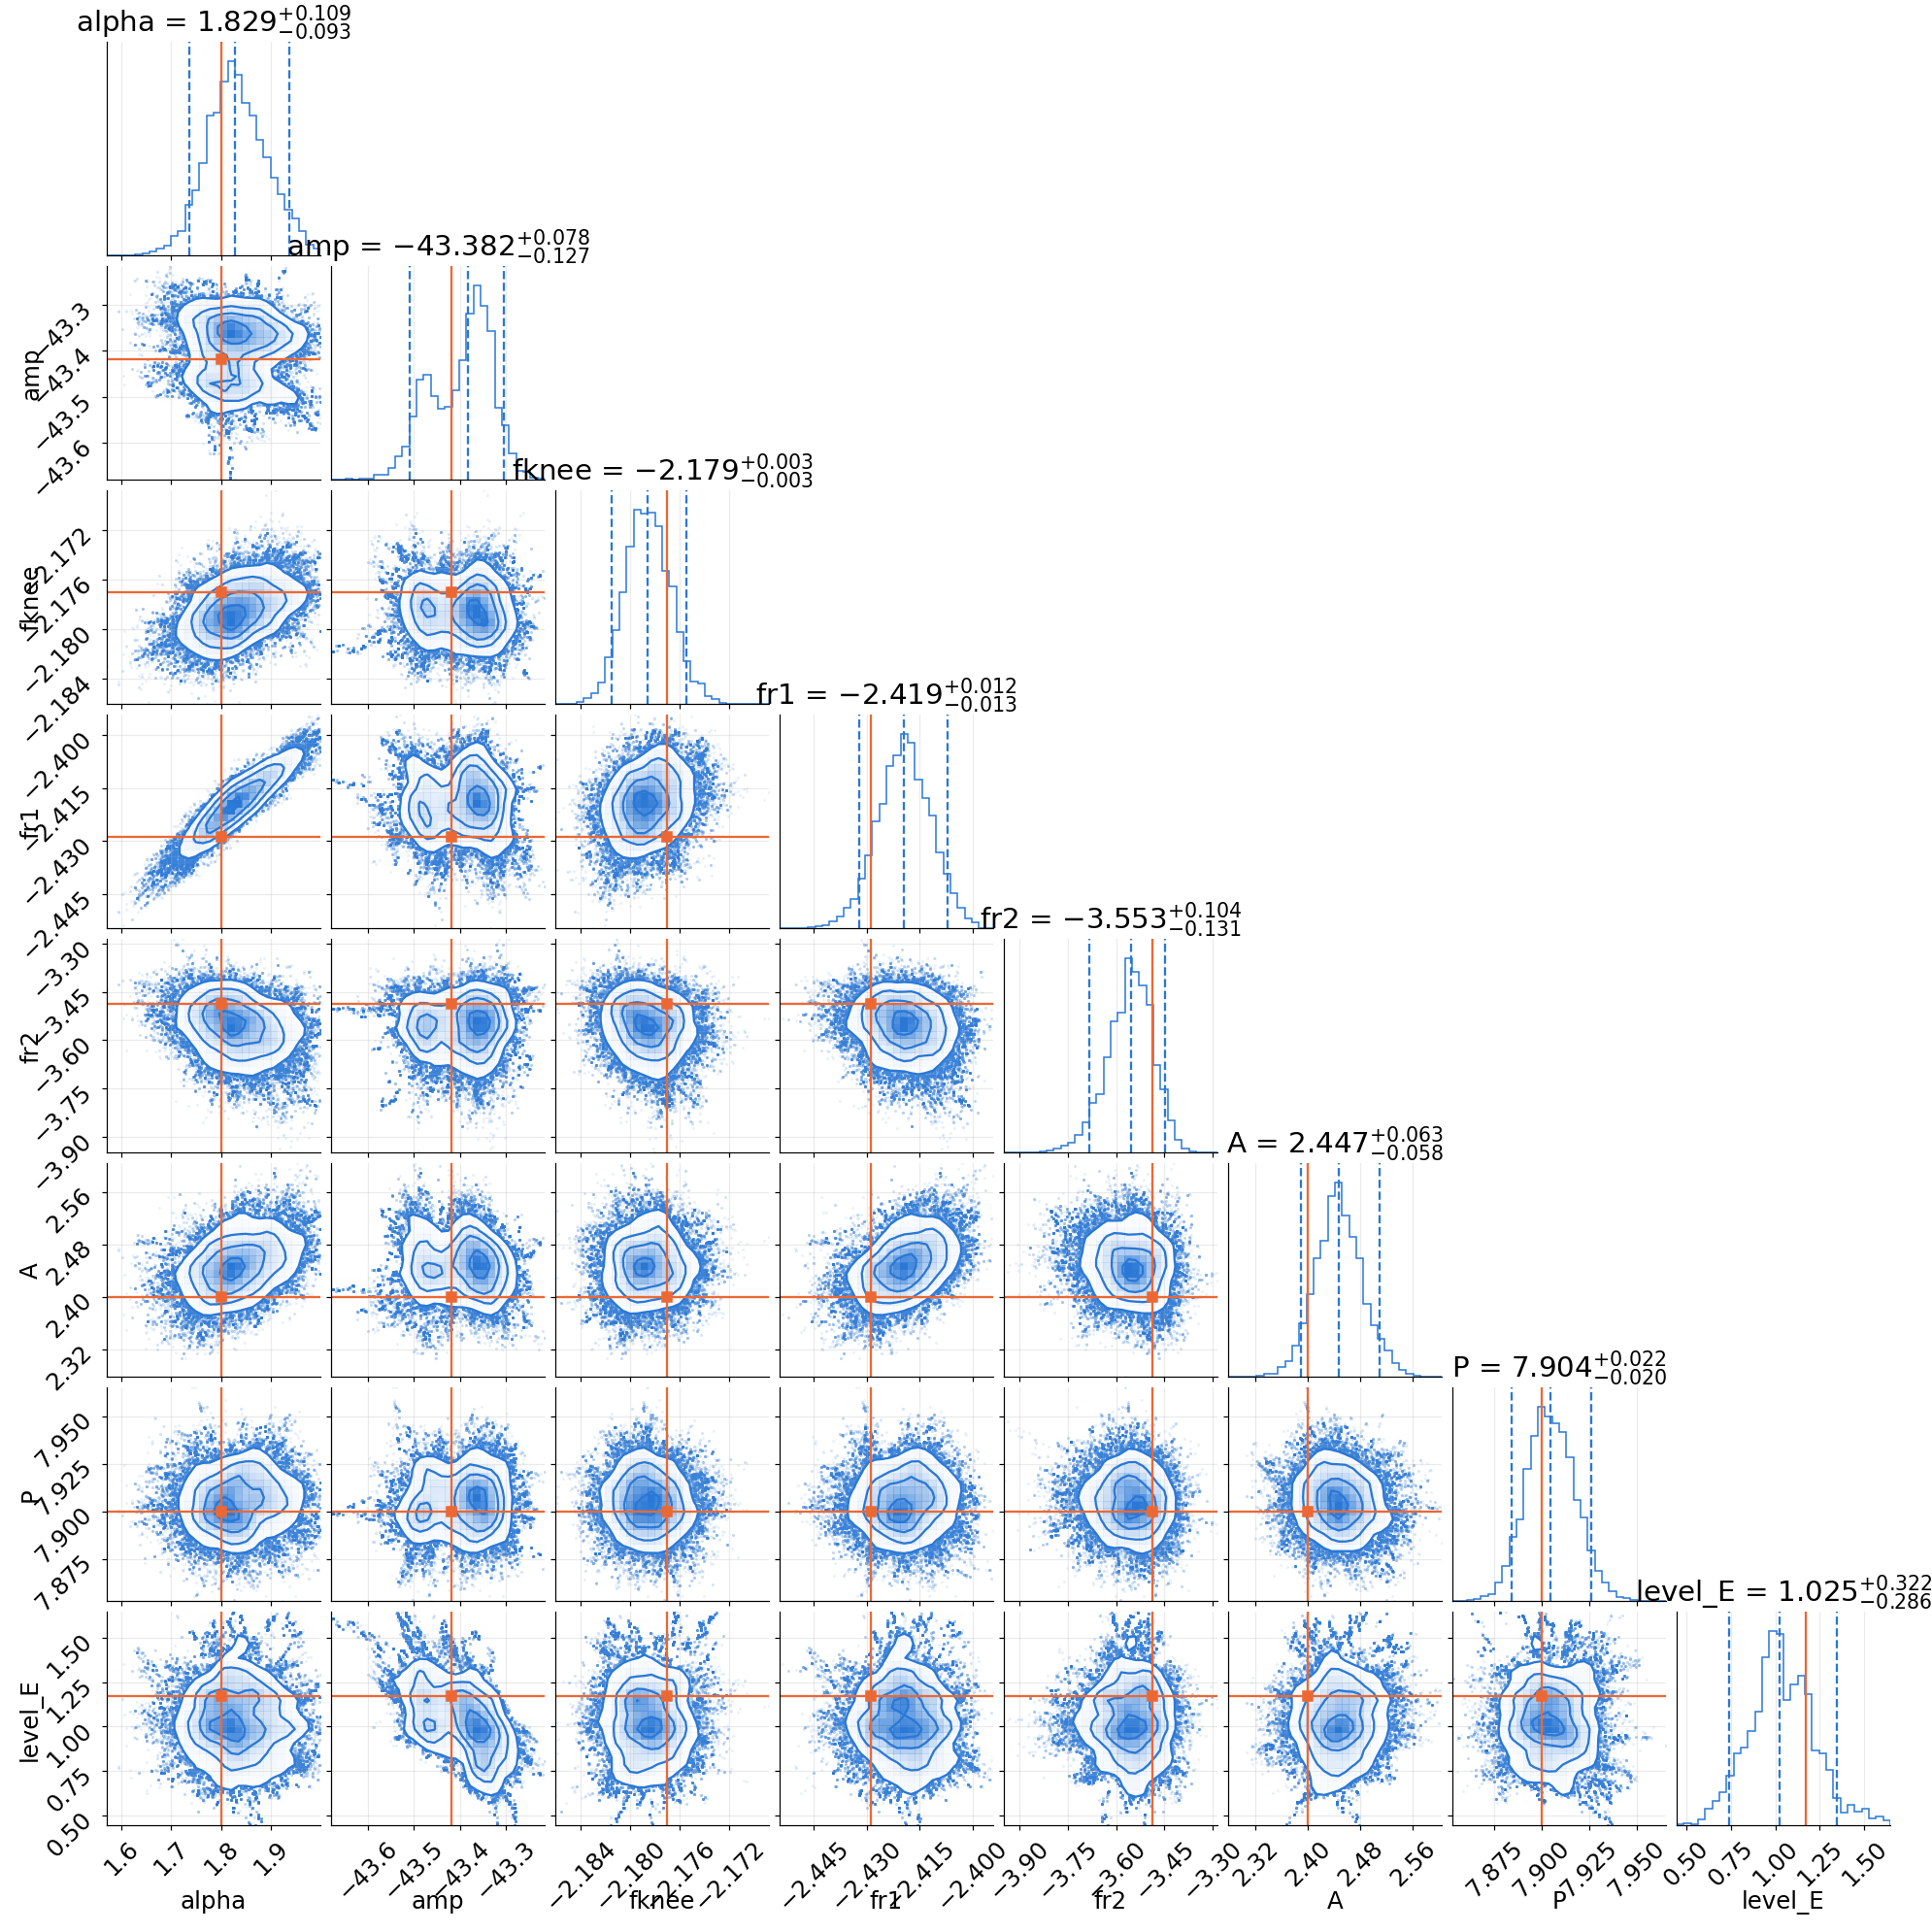
\includegraphics[width=0.8\textwidth]{figures/run1_corner.png}
\caption{Run~1: posterior of the spectral parameters and \texttt{level\_E}; orange
lines are the injected values. The double peak in \texttt{amp} is the trade-off with
the spectral shape and with the atoms.}
\label{fig:run1corner}
\end{figure}

%============================================================================
\section{Run 2: the true envelope, wavelets against chunks}
%============================================================================

\paragraph{Set-up.} The Galactic foreground is modulated by the true sky envelope
$M_j^2(t)$, which no finite set of atoms represents exactly. The \emph{same} series is
analysed with the wavelet RJMCMC (free atoms) and with the chunked pipeline of
Part~I (two 15-day chunks with a 5\% Tukey taper, 1000 log bins, the 5-parameter sky
envelope, \texttt{nessai}). The chunked likelihood is run twice: with the paper's
shape $n_b/2$ and with the correct $n_b$ (\cref{sec:dofbug}).

\begin{figure}[t]
\centering
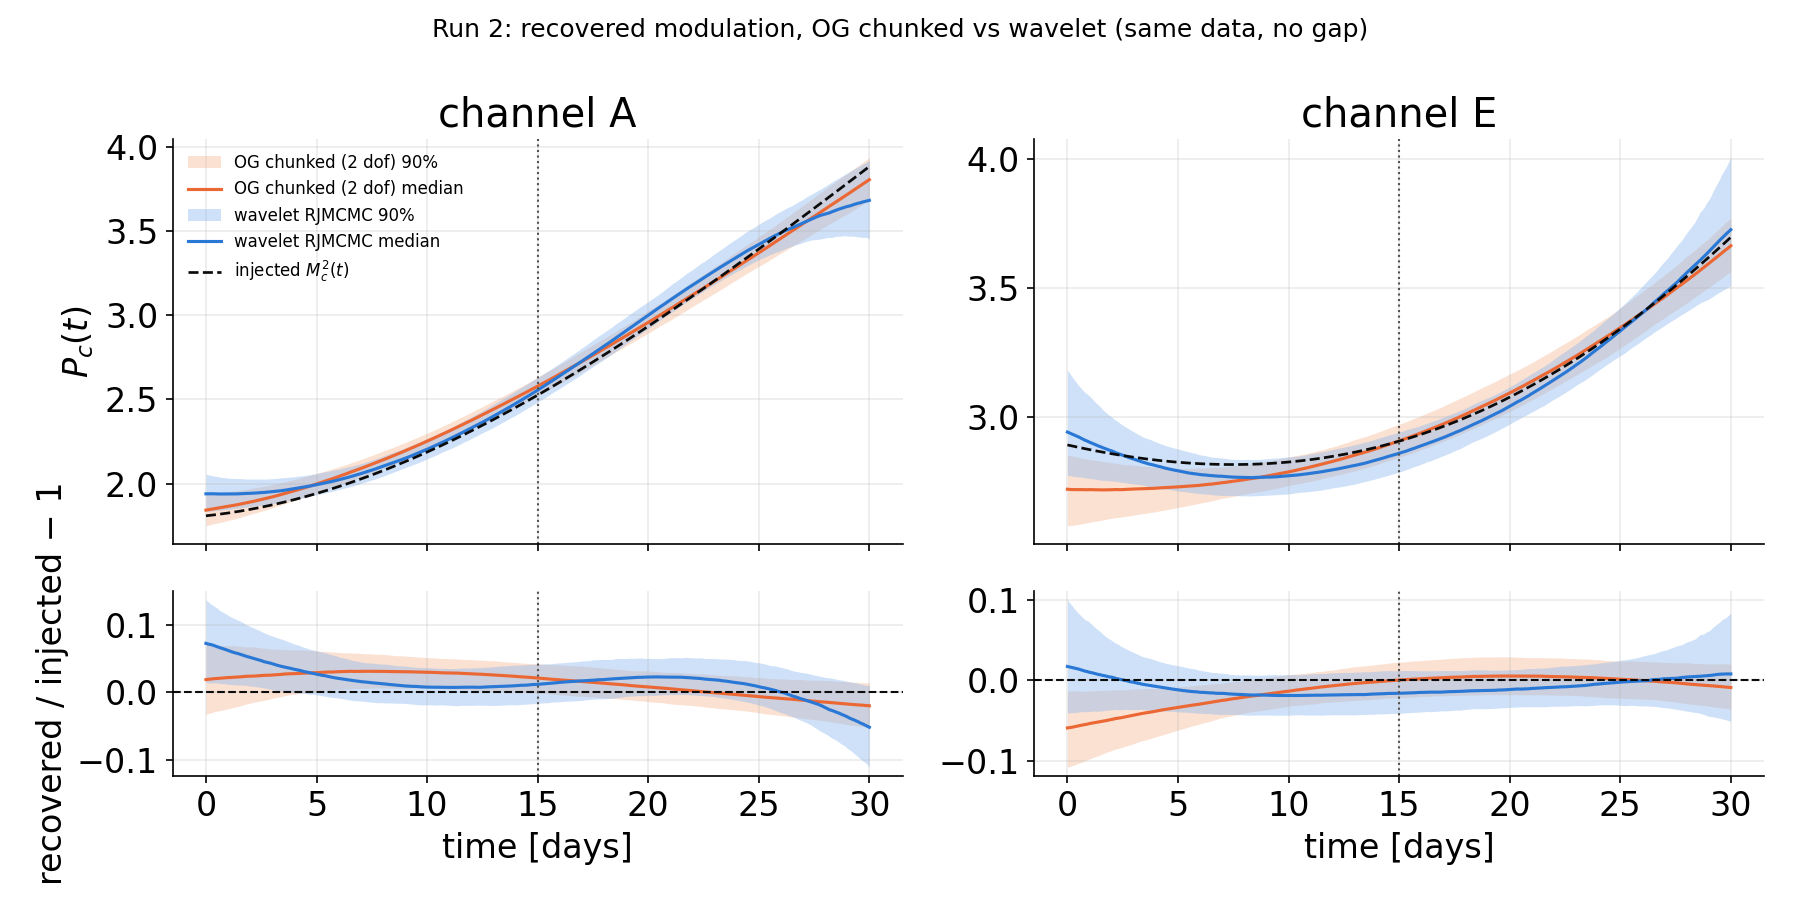
\includegraphics[width=\textwidth]{figures/run2_modulation.png}
\caption{Run~2: recovered $P_j(t)$ on the injected scale, chunked pipeline with the
correct degrees of freedom (orange) and wavelet RJMCMC (blue), 90\% bands; dashed: the
injected envelope. Bottom: recovered/injected $-1$. The dotted line marks the
boundary between the two chunks.}
\label{fig:run2mod}
\end{figure}

\paragraph{Results.}
\begin{itemize}
  \item \textbf{Spectral parameters} (\cref{fig:run2corner}): the three posteriors agree
        on the medians (same data), all $|z|\le1.35$. The wavelet widths are 1.00--1.13
        times those of the corrected chunked run. With the paper's shape $n_b/2$ the
        chunked widths are 1.34--1.43 $\approx\sqrt2$ larger, as \cref{sec:dofbug}
        predicts.
  \item \textbf{Galactic brightness} (\cref{fig:run2mod}): 90\% bands of 5.8\% (A) and
        5.2\% (E) for the wavelet model, against 4.8\% and 4.6\% for the corrected
        chunked model, i.e.\ 12--20\% wider. The difference sits mostly at the ends of
        the window, where the wavelet model has fewer pixels and the atoms
        extrapolate; in the middle the widths are close.
  \item \textbf{Time dependence alone} (each draw divided by its own 30-day mean): the
        wavelet bands are 1.3--1.5 times wider. The sky model ties both channels to
        five parameters, while free atoms fit each channel's shape on its own. This is
        the price of not assuming the Galaxy's shape.
\end{itemize}
The chunked sky parameters are all within 1.4$\sigma$ of the truth but broad
($\sin\psi\in[-0.95,-0.52]$ at 90\%): 30 days constrain the envelope's shape, not each
sky parameter.

\begin{figure}[t]
\centering
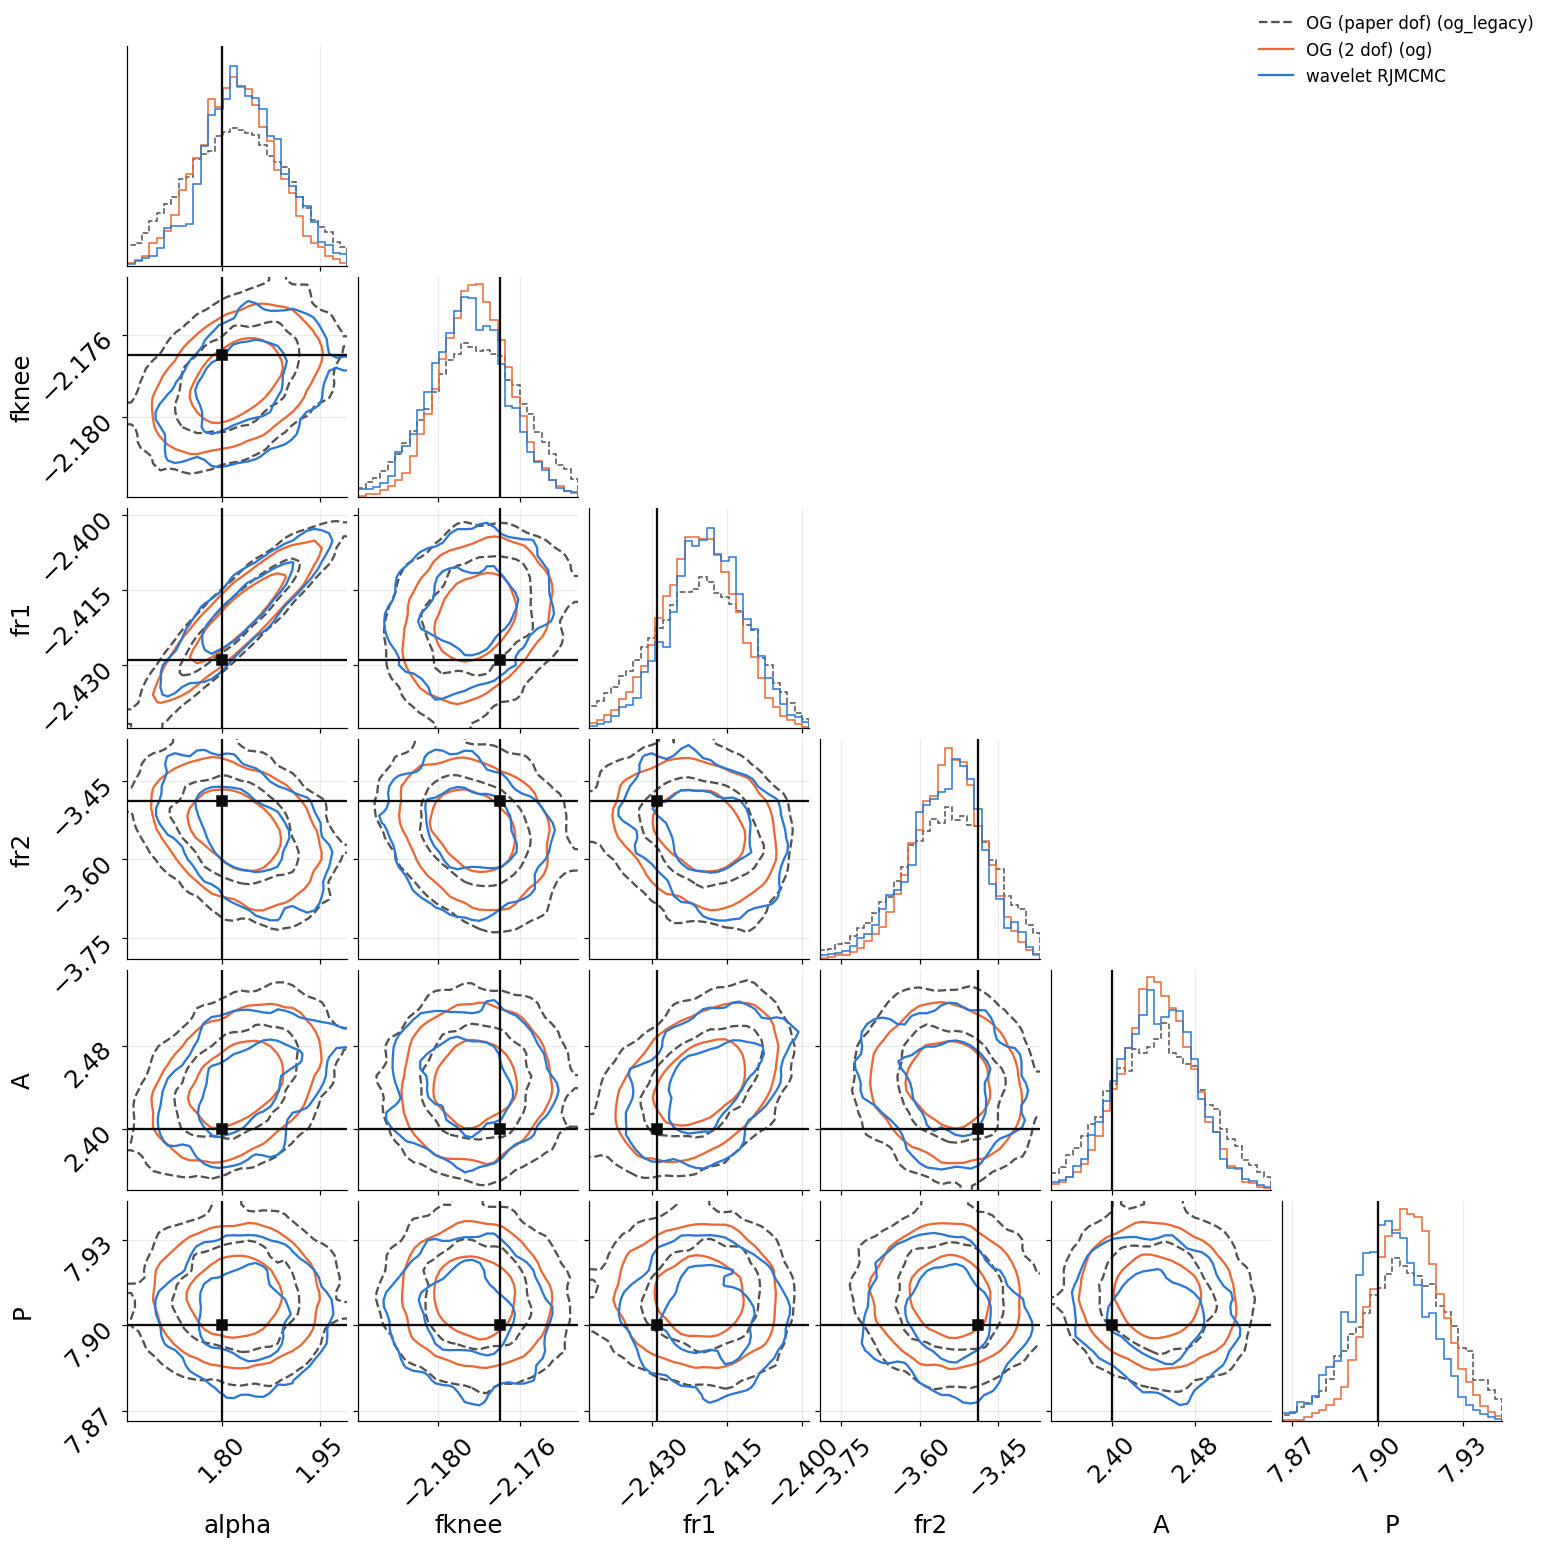
\includegraphics[width=0.75\textwidth]{figures/run2_corner.png}
\caption{Run~2: spectral parameters shared by both models. Grey dashed: chunked
pipeline with the paper's degrees of freedom; orange: chunked with the correct ones;
blue: wavelet RJMCMC. Black lines: injected values.}
\label{fig:run2corner}
\end{figure}

%============================================================================
\section{Runs 3 and 4: a one-day and a ten-day gap}
%============================================================================

\paragraph{Set-up.} Run~2's series with a 1-day (run~3) or 10-day (run~4) gap,
masked as in \cref{sec:gapmask} (\cref{fig:gapmask}). The sampler, priors and seeds are
those of run~2, so the comparison with run~2's wavelet posterior isolates the effect
of the gap.

\paragraph{Spectral parameters} (\cref{fig:gapcorner}). The 1-day gap widens them by
0--8\%, the 10-day gap by 11--32\%. The expectation from the lost pixels,
$\sqrt{1/(1-f_{\rm lost})}$, is 4\% and 29\%. All medians stay within 0.7$\sigma$ of
run~2's.

\begin{figure}[t]
\centering
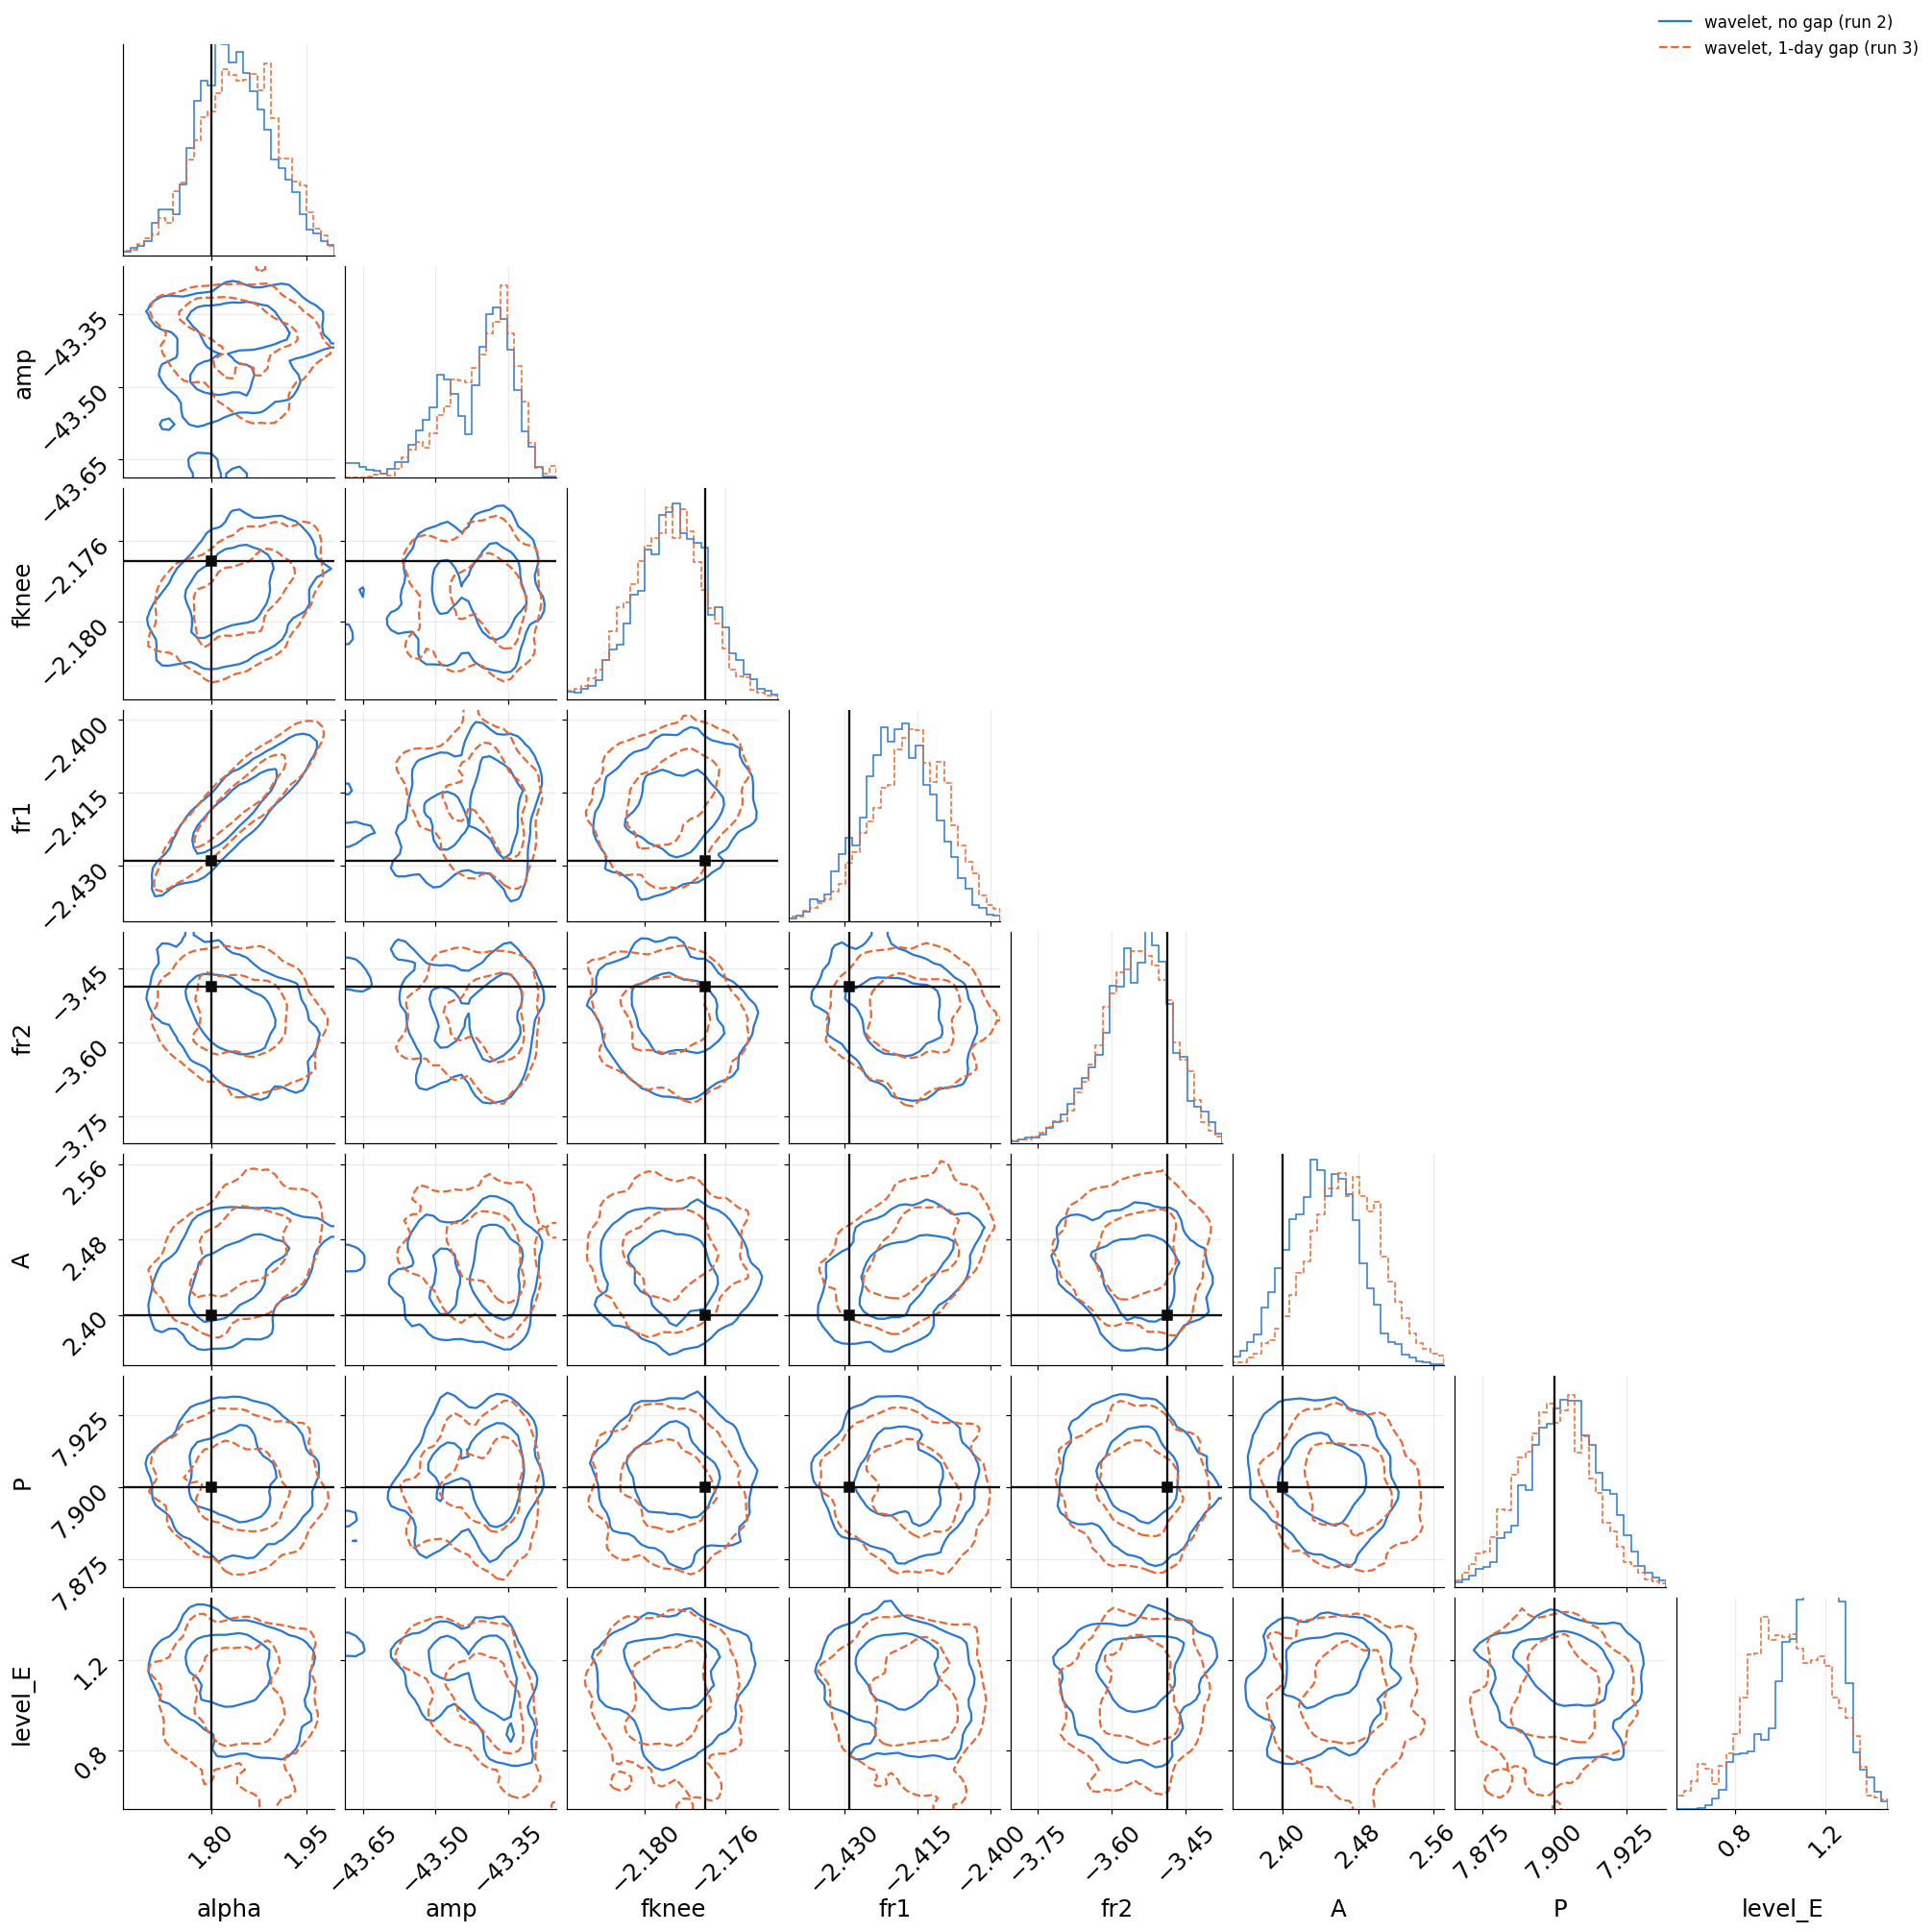
\includegraphics[width=0.49\textwidth]{figures/run3_corner.png}\hfill
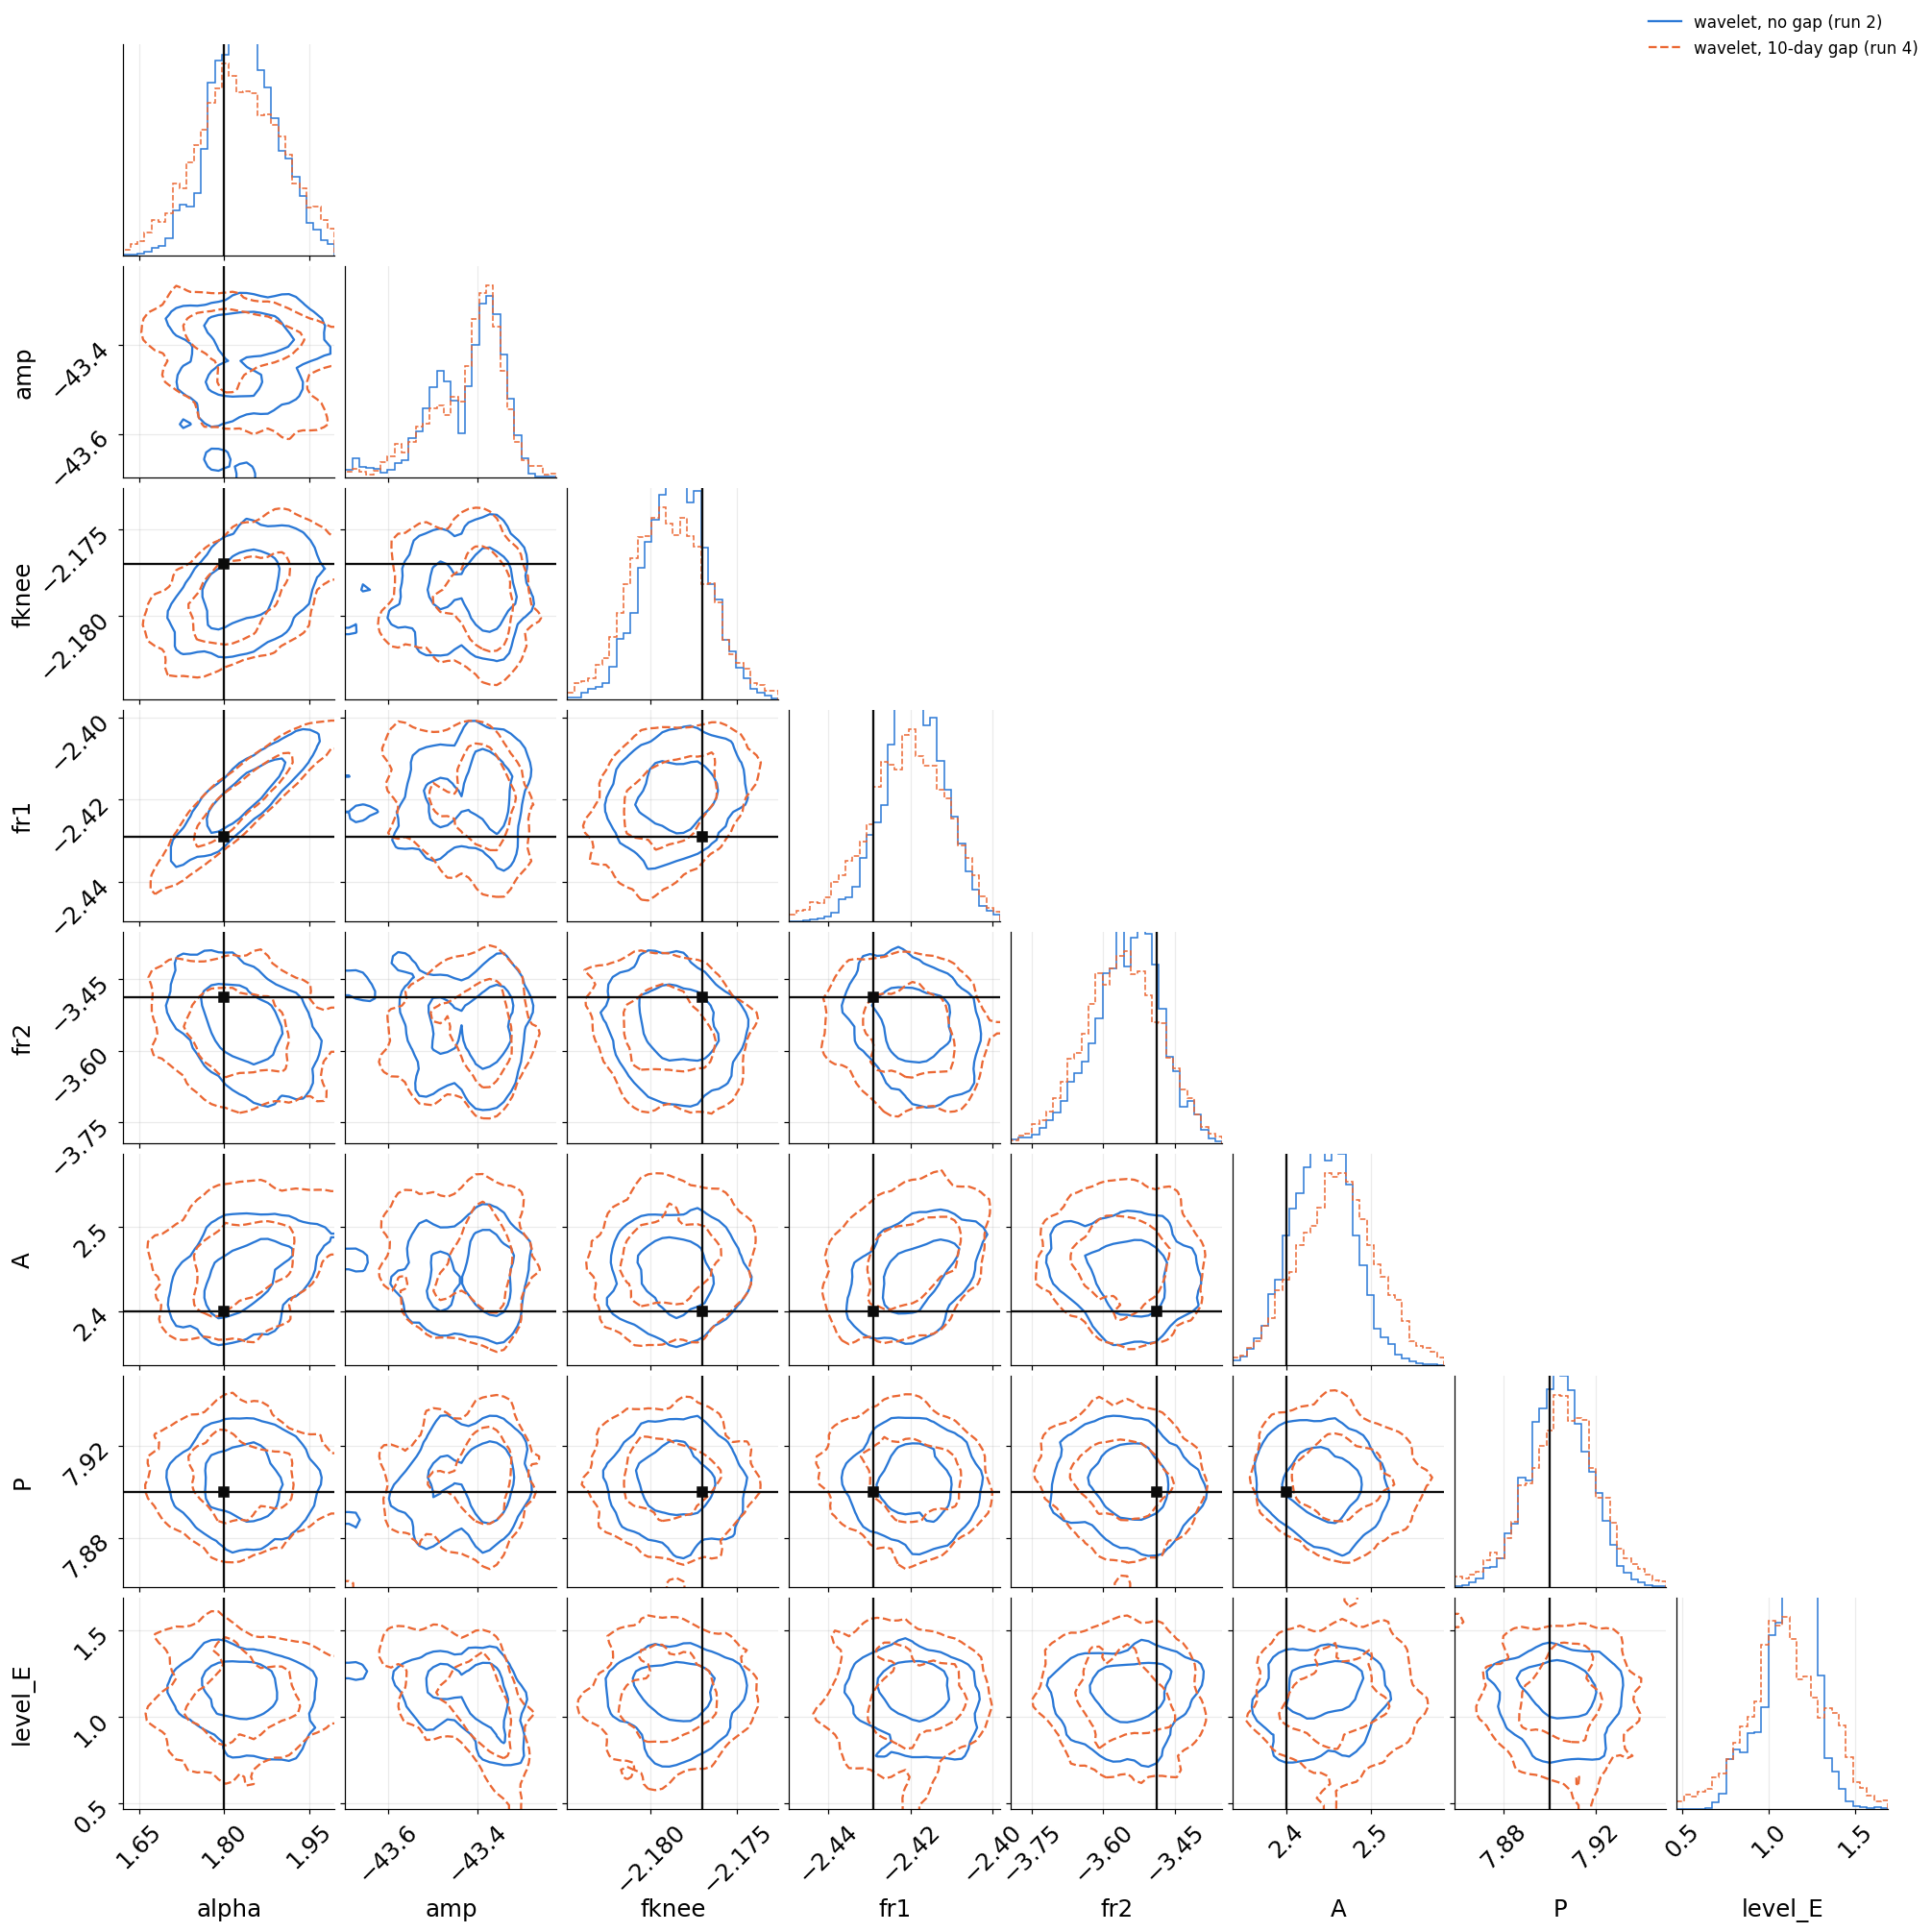
\includegraphics[width=0.49\textwidth]{figures/run4_corner.png}
\caption{Spectral posteriors with a gap (orange dashed) against run~2 without a gap
(blue). Left: run~3, 1-day gap. Right: run~4, 10-day gap. Black lines: injected
values.}
\label{fig:gapcorner}
\end{figure}

\paragraph{The modulation through the gap.} As explained in \cref{sec:gapmod}, the
atoms define $P_j(t)$ inside the gap without any data there.
\begin{itemize}
  \item \textbf{1-day gap:} the band widens only locally, by 0.3--0.4 percentage
        points (from 5.9 to 6.2\% in A, 5.4 to 5.8\% in E), and the median follows
        run~2's within 0.5\%. Atoms 20--35\,d wide bridge 50\,h with almost no extra
        freedom.
  \item \textbf{10-day gap} (\cref{fig:run4mod}): the band grows steadily into the gap
        and peaks in its middle, at 14.5\% (A) and 12.9\% (E) against 5.8\% and 5.3\%
        without the gap, about 2.5 times wider. The median follows run~2's within 1\%,
        and the truth stays inside the 90\% band throughout the gap in both channels.
        The kept data widen slightly too (6.1 to 7.5\% in A over 3--27\,d), because the
        shared spectral parameters are less well measured.
\end{itemize}
Neither gap introduces a bias. A gap costs what the missing data account for, plus an
interpolation uncertainty inside the gap that the posterior reports honestly.

\begin{figure}[t]
\centering
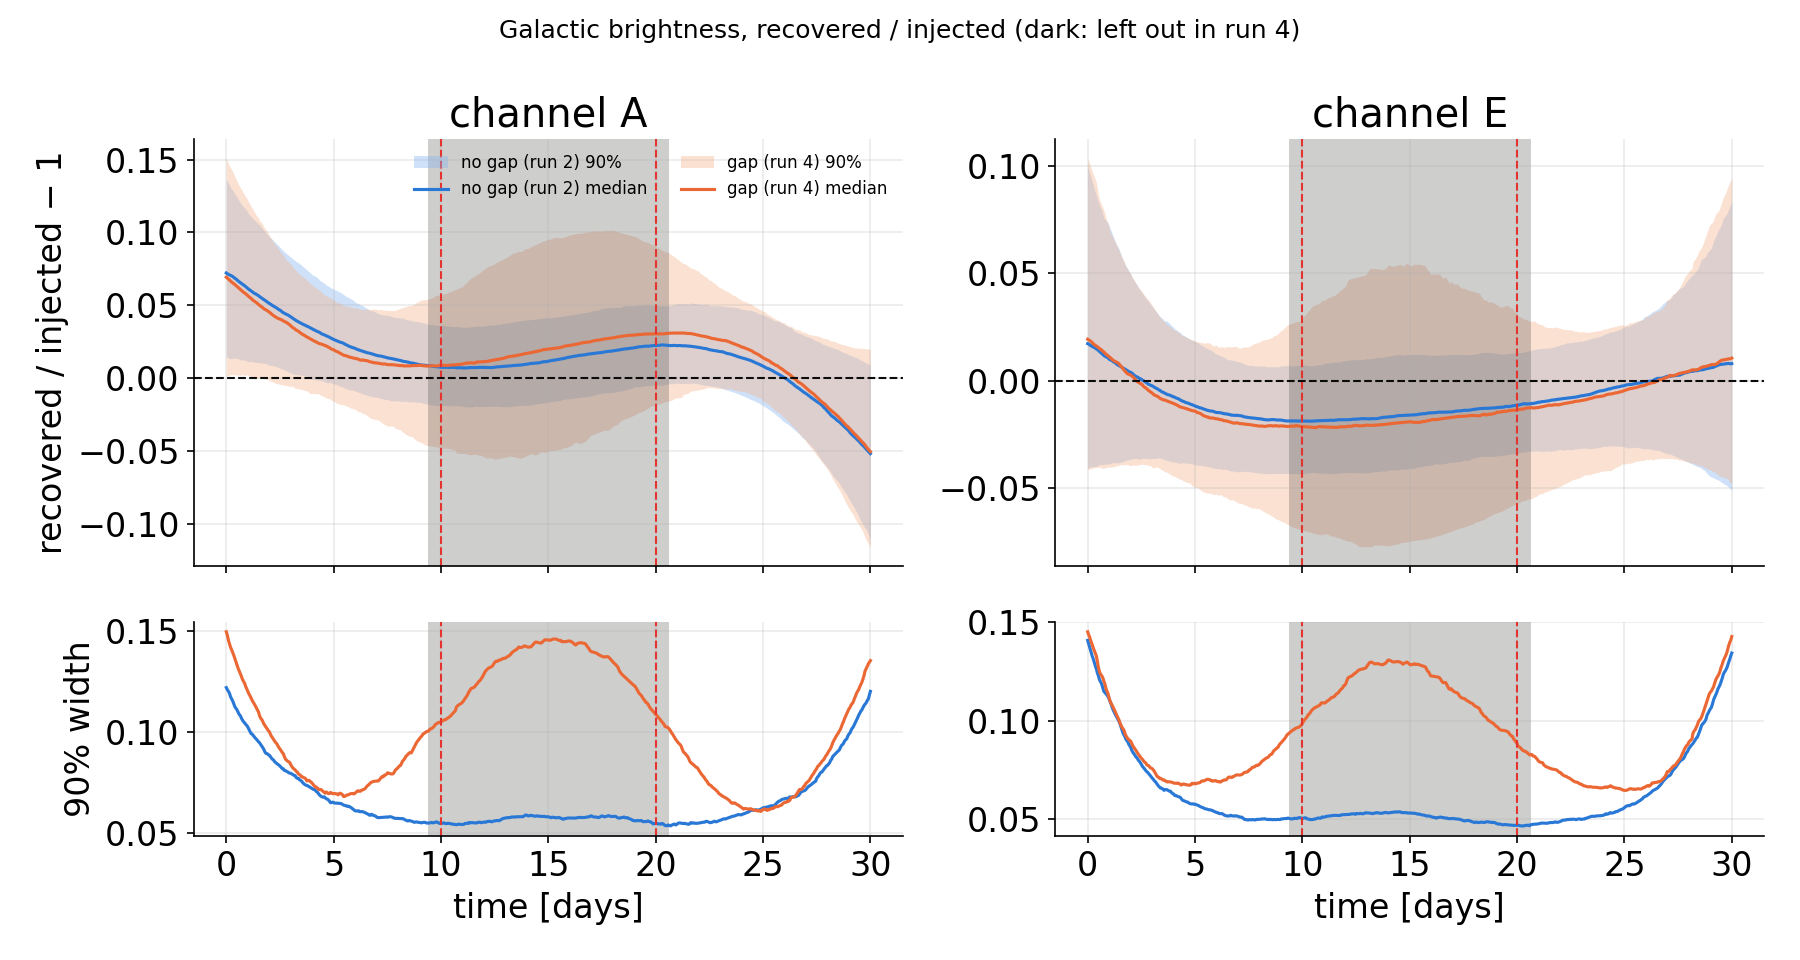
\includegraphics[width=\textwidth]{figures/run4_modulation.png}
\caption{Run~4: galactic brightness recovered/injected $-1$ with the 10-day gap
(orange) and without it (run~2, blue). Grey: the columns left out of the likelihood;
red dashed: the gap. Inside the grey region the curve is the atom model continued
through the gap, constrained only by the data on either side. Bottom: width of the
90\% band.}
\label{fig:run4mod}
\end{figure}

%============================================================================
\section{Run 5: a Galaxy with four bright patches}
%============================================================================

\paragraph{Set-up.} The sky of \cref{sec:patchsim} (\cref{fig:sky}), analysed on the
same WDM pixels with two models of $P_j(t)$: the atoms in time of runs~1--4, and the
5a patch fit of \cref{sec:run5a}.

\paragraph{The total modulation} (\cref{fig:run5corner}). Both models recover the
30-day mean galactic brightness to within 1.5\% in A and 1.2\% in E, with the same
90\% width (3.2\%). The spectral parameters agree, with width ratios 5a/atoms of
0.88--1.06. Along time, the 5a band is somewhat narrower (4.2--4.3\% against
4.9--5.6\%), as expected from a model that knows the sky. Even a large departure from
the Gaussian Galaxy (+85\% of power in A) is therefore absorbed by the atoms without
bias: they describe $P_j(t)$, whatever its origin.

\begin{figure}[t]
\centering
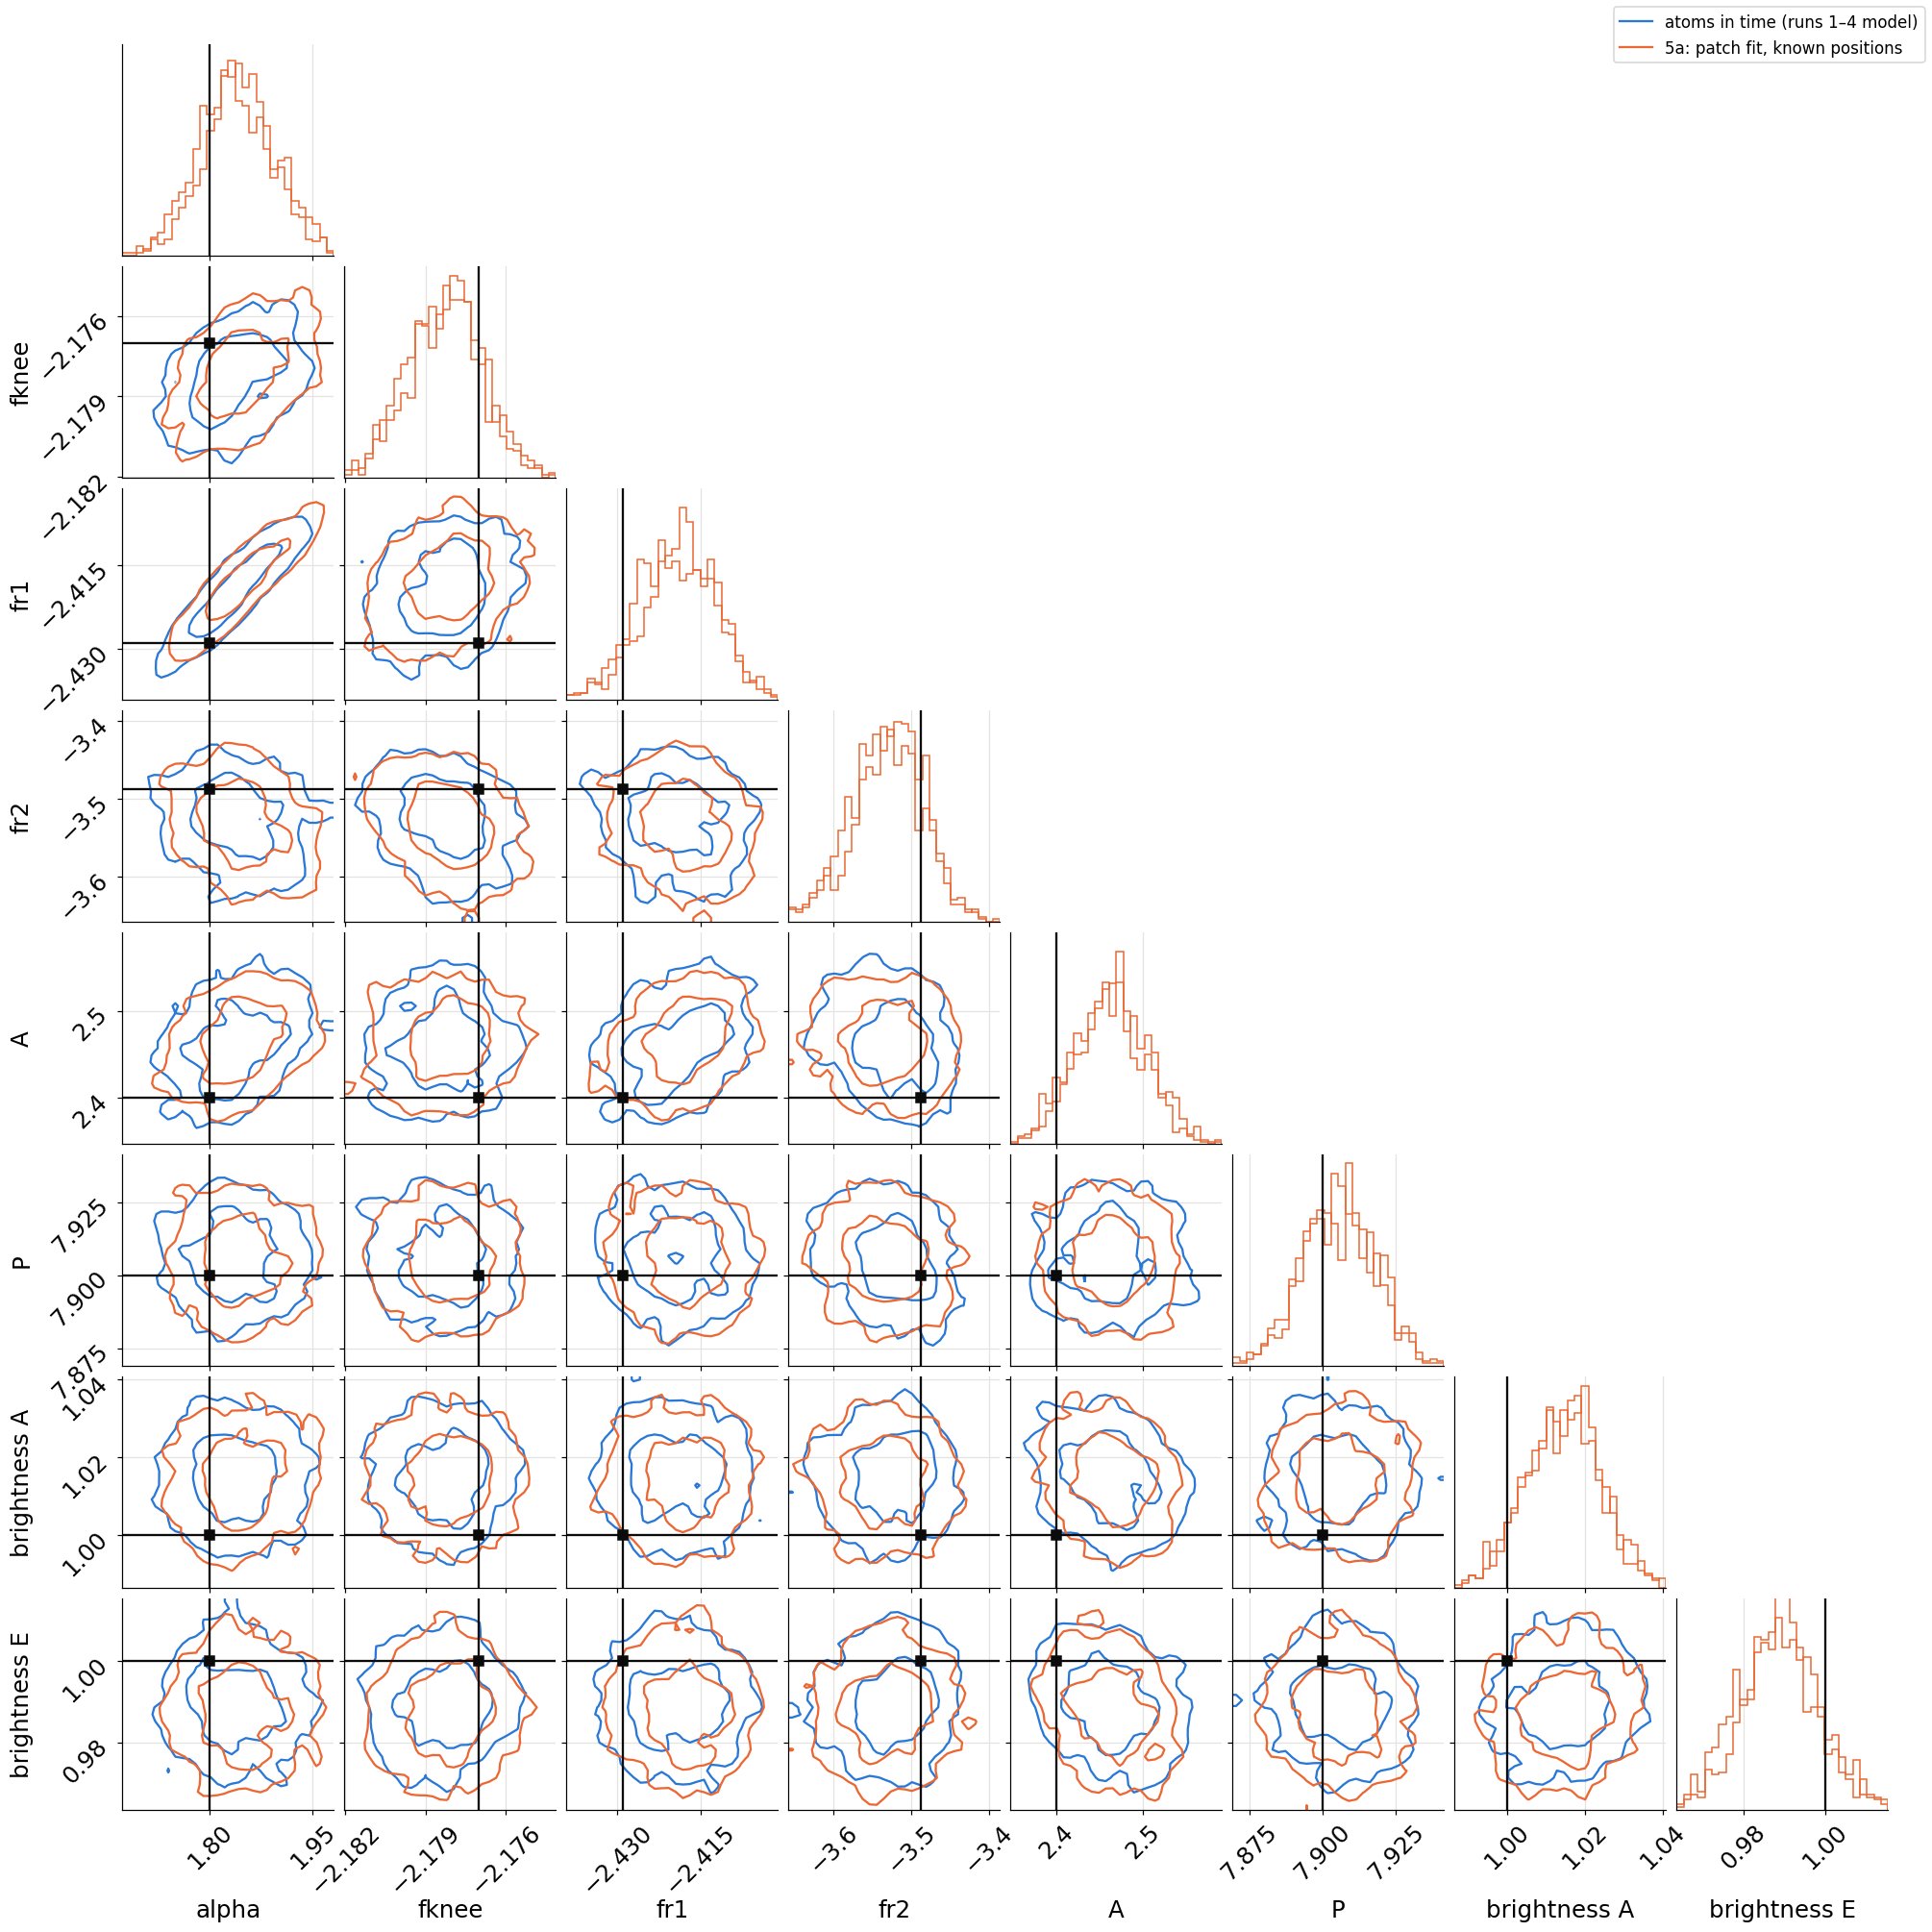
\includegraphics[width=0.8\textwidth]{figures/run5_corner.png}
\caption{Run~5: atoms in time (blue) and the 5a patch fit at known positions (orange)
on the same data, for the shared spectral parameters and the 30-day mean galactic
brightness in A and E (recovered/injected). Black lines: injected values.}
\label{fig:run5corner}
\end{figure}

\paragraph{The individual patches.} Detection significance is the posterior median
over its standard deviation:
\begin{center}
\small
\begin{tabular}{@{}lccccc@{}}
\toprule
patch & true $F_i$ & median & 90\% interval & median/std & (median$-$truth)/std \\
\midrule
LMC & 0.20 & 0.133 & [0.013, 0.331] & 1.4 & $-0.69$ \\
SMC & 0.08 & 0.118 & [0.047, 0.181] & 2.9 & $+0.92$ \\
Sgr dSph & 0.12 & 0.227 & [0.055, 0.434] & 1.9 & $+0.92$ \\
bar end & 0.12 & 0.200 & [0.122, 0.274] & 4.3 & $+1.71$ \\
\bottomrule
\end{tabular}
\end{center}
All four fluxes are consistent with the truth, but only the bar end, the one patch in
the plane and away from the centre, is clearly detected. The fluxes are strongly
anticorrelated (LMC with the others, $-0.6$ to $-0.75$). The reason is the template
overlap of \cref{sec:run5a}: alone, each flux would be measured to 0.02--0.07; with all
four free, the errors grow two to four times. The data measure about two flux
combinations well (errors 0.020 and 0.025) and the other two poorly (0.07 and 0.25).
\emph{Even in the best case, 30 days measure how much excess there is, not where it
comes from.}

\clearpage
%############################################################################
\part{Conclusions and outlook}
%############################################################################

\section{Conclusions}

\begin{itemize}
  \item \textbf{The WDM likelihood is the chunked likelihood in another domain.} The
        Gamma likelihood of grouped WDM pixels is \PoneEq{9} applied to wavelet
        periodograms, with 20-h time blocks in place of chunks. The derivation shows
        that \PoneEq{9} (and the chunked samplers of \texttt{bahamas}) uses half the
        correct degrees of freedom, which makes chunked posteriors $\sqrt2$ too wide.
  \item \textbf{A free modulation is recovered without bias.} Gaussian atoms with a
        variable number, sampled by reversible jump, recover the galactic brightness to
        1--2\% with 5--6\% bands over 30 days, both for an atom injection and for the
        true sky envelope. The number of atoms is not identifiable, and need not be.
  \item \textbf{Its price is modest.} Against the 5-parameter sky model on the same
        data, the wavelet brightness bands are 12--20\% wider and the time dependence
        alone 1.3--1.5 times wider, mostly at the ends of the window. The spectral
        parameters are measured equally well.
  \item \textbf{Gaps are handled exactly by masking.} Leaving out the gap columns and
        one buffer column per side keeps the likelihood exact. A 1-day gap costs almost
        nothing; a 10-day gap widens the spectral parameters as the lost data predict
        and the modulation band inside the gap by 2.5 times, without bias.
  \item \textbf{The sky is seen only through $\ell=0,2,4$.} A patchy Galaxy changes
        $P_j(t)$ strongly, and the atoms absorb it without bias. Even with positions
        known, the fluxes of individual patches are barely separable in 30 days.
        Needlets make the reason explicit and reduce a sky model to 241 coefficients in
        three bands.
\end{itemize}

\section{Discussion and next steps}

\paragraph{From 30 days to four years.} Everything above uses 30 days, over which the
envelope is a smooth, nearly quadratic curve and the constellation normal turns by
only about 30\textdegree. The next step is to apply the pipeline to four years of mock
LISA data. Over that span the modulation goes through eight cycles, the atom model
must describe a periodic signal with many more atoms, and the sky model gains the most:
as the normal precesses through 360\textdegree, the ring degeneracy of patch positions
should break, and the needlet coefficients in bands $j=1,2$ should become measurable.
The likelihood scales linearly with the number of time blocks and should remain
cheap; we expect the transdimensional sampling to be the bottleneck. Runs~5b (free positions) and 5c
(needlet coefficients) will be done on both time scales.

\paragraph{Better handling of gaps.} Runs~3 and 4 place one hard-edged gap in the
middle of the window. Open tests are: the realistic LISA gap pattern (short scheduled
gaps every two weeks plus random unscheduled ones, a 75\% duty cycle); a long gap at
the start or end of the window, where the atoms extrapolate instead of interpolate;
tapered gap edges, which should remove the low-frequency leakage and shrink the
buffer; letting atom centres lie outside the window, which should cure the excess at
the window ends seen in every run; and the chunked pipeline on the same gapped data,
where a short gap can cost most of a chunk.

\paragraph{Comparison with CTMCMC.} The number of atoms (and later of sky
components) is sampled here with birth--death reversible-jump moves in \texttt{eryn}:
a birth or death is proposed at discrete steps and accepted or rejected with a
Metropolis--Hastings probability. \texttt{samsara}
(\href{https://arxiv.org/abs/2511.07385}{Astorino et al.\ 2025}) is a continuous-time
MCMC (CTMCMC) sampler built for the same kind of transdimensional problem, with the
LISA global fit as its motivation. Following the birth--death process of
\href{https://doi.org/10.1214/aos/1016120364}{Stephens (2000)}, components are born,
die and mutate as Poisson events in continuous time. The rates are chosen so that
detailed balance holds, and every transdimensional move is then accepted; the
posterior is obtained by weighting each state by the time the chain spends in it. This
removes the low acceptance of birth and death moves (0.7--1\% in our runs), which is
the main limit on how fast the reversible-jump chain explores $K$. We plan to fit the
atom model, and later the needlet sky model, with both samplers on the same data and
compare the posteriors on the modulation, the mixing in $K$, and the cost per
independent sample.

%============================================================================
\section*{References}
%============================================================================
\begin{itemize}\sloppy
  \item R.~Buscicchio, F.~Pozzoli, D.~Chirico, A.~Sesana, \emph{The first year of LISA
        Galactic foreground},
        \href{https://arxiv.org/abs/2511.03604}{arXiv:2511.03604}.
  \item R.~Buscicchio, A.~Klein, V.~Korol, F.~Di~Renzo, C.~J.~Moore, D.~Gerosa,
        A.~Carzaniga, \emph{Test for LISA foreground Gaussianity and stationarity:
        galactic white-dwarf binaries}, Eur.\ Phys.\ J.\ C \textbf{85}, 887 (2025),
        \href{https://arxiv.org/abs/2410.08263}{arXiv:2410.08263}.
  \item N.~Karnesis, S.~Babak, M.~Pieroni, N.~Cornish, T.~Littenberg,
        \emph{Characterization of the stochastic signal originating from compact
        binaries populations as measured by LISA}, Phys.\ Rev.\ D \textbf{104},
        043019 (2021), \href{https://arxiv.org/abs/2103.14598}{arXiv:2103.14598}.
  \item G.~Casella, R.~L.~Berger, \emph{Statistical Inference}, 2nd ed., Duxbury (2002),
        Sec.~3.3.
  \item NIST/SEMATECH e-Handbook of Statistical Methods,
        \href{https://www.itl.nist.gov/div898/handbook/eda/section3/eda366b.htm}{Gamma distribution}.
  \item M.~D.~Hoffman, A.~Gelman, \emph{The No-U-Turn Sampler}, JMLR \textbf{15}, 1593
        (2014), \href{https://arxiv.org/abs/1111.4246}{arXiv:1111.4246}.
  \item D.~Phan, N.~Pradhan, M.~Jankowiak, \emph{Composable effects for flexible and
        accelerated probabilistic programming in NumPyro},
        \href{https://arxiv.org/abs/1912.11554}{arXiv:1912.11554}.
  \item M.~J.~Williams, J.~Veitch, C.~Messenger, \emph{Nested sampling with normalizing
        flows for gravitational-wave inference}, Phys.\ Rev.\ D \textbf{103}, 103006
        (2021), \href{https://arxiv.org/abs/2102.11056}{arXiv:2102.11056}.
  \item N.~J.~Cornish, \emph{Time-frequency analysis of gravitational wave data},
        Phys.\ Rev.\ D \textbf{102}, 124038 (2020),
        \href{https://arxiv.org/abs/2009.00043}{arXiv:2009.00043}.
  \item V.~Necula, S.~Klimenko, G.~Mitselmakher, \emph{Transient analysis with fast
        Wilson-Daubechies time-frequency transform}, J.\ Phys.\ Conf.\ Ser.\
        \textbf{363}, 012032 (2012),
        \href{https://doi.org/10.1088/1742-6596/363/1/012032}{doi:10.1088/1742-6596/363/1/012032}.
  \item I.~Daubechies, S.~Jaffard, J.-L.~Journ\'e, \emph{A simple Wilson orthonormal
        basis with exponential decay}, SIAM J.\ Math.\ Anal.\ \textbf{22}, 554 (1991),
        \href{https://doi.org/10.1137/0522035}{doi:10.1137/0522035}.
  \item I.~Daubechies, \emph{Ten Lectures on Wavelets}, SIAM (1992) (the Balian--Low
        theorem).
  \item M.~C.~Digman, N.~J.~Cornish, \emph{LISA gravitational wave sources in a
        time-varying galactic stochastic background},
        \href{https://arxiv.org/abs/2212.04600}{arXiv:2212.04600}.
  \item N.~Pearson, N.~J.~Cornish, \emph{Handling data gaps for the next generation of
        gravitational-wave observatories},
        \href{https://arxiv.org/abs/2509.05479}{arXiv:2509.05479}.
  \item P.~J.~Green, \emph{Reversible jump Markov chain Monte Carlo computation and
        Bayesian model determination}, Biometrika \textbf{82}, 711 (1995),
        \href{https://doi.org/10.1093/biomet/82.4.711}{doi:10.1093/biomet/82.4.711}.
  \item N.~Karnesis, M.~L.~Katz, N.~Korsakova, J.~R.~Gair, N.~Stergioulas,
        \emph{Eryn: a multi-purpose sampler for Bayesian inference}, MNRAS (2023),
        \href{https://arxiv.org/abs/2303.02164}{arXiv:2303.02164}.
  \item J.~Goodman, J.~Weare, \emph{Ensemble samplers with affine invariance}, Commun.\
        Appl.\ Math.\ Comput.\ Sci.\ \textbf{5}, 65 (2010),
        \href{https://doi.org/10.2140/camcos.2010.5.65}{doi:10.2140/camcos.2010.5.65}.
  \item F.~J.~Narcowich, P.~Petrushev, J.~D.~Ward, \emph{Localized tight frames on
        spheres}, SIAM J.\ Math.\ Anal.\ \textbf{38}, 574 (2006),
        \href{https://doi.org/10.1137/040614359}{doi:10.1137/040614359}.
  \item D.~Marinucci et al., \emph{Spherical needlets for cosmic microwave background
        data analysis}, MNRAS \textbf{383}, 539 (2008),
        \href{https://arxiv.org/abs/0707.0844}{arXiv:0707.0844}.
  \item P.~Baldi, G.~Kerkyacharian, D.~Marinucci, D.~Picard, \emph{Asymptotics for
        spherical needlets}, Ann.\ Statist.\ \textbf{37}, 1150 (2009),
        \href{https://doi.org/10.1214/08-AOS601}{doi:10.1214/08-AOS601}.
  \item K.~M.~G\'orski et al., \emph{HEALPix: a framework for high-resolution
        discretization and fast analysis of data distributed on the sphere}, ApJ
        \textbf{622}, 759 (2005),
        \href{https://arxiv.org/abs/astro-ph/0409513}{arXiv:astro-ph/0409513}.
  \item M.~Stephens, \emph{Bayesian analysis of mixture models with an unknown number of
        components---an alternative to reversible jump methods}, Ann.\ Statist.\
        \textbf{28}, 40 (2000),
        \href{https://doi.org/10.1214/aos/1016120364}{doi:10.1214/aos/1016120364}.
  \item G.~Astorino, L.~Valbusa Dall'Armi, R.~Buscicchio, J.~Pomper, A.~Ricciardone,
        W.~Del Pozzo, \emph{samsara: A Continuous-Time Markov Chain Monte Carlo Sampler
        for Trans-Dimensional Bayesian Analysis},
        \href{https://arxiv.org/abs/2511.07385}{arXiv:2511.07385}.
\end{itemize}

\end{document}
